\documentclass[letterpaper,12pt,twoside]{book}
%\documentclass[draft,letterpaper,12pt,twoside]{book}
%%%%%%%%%%%%%%%%%%%%%%%%%%%%%% Pacotes: básicos %%%%%%%%%%%%%%%%%%%%%%%%%%%%%% 
\usepackage[utf8]{inputenc}
\usepackage{cmap}
\usepackage[T1]{fontenc}
\usepackage[english,brazilian]{babel}
\usepackage{indentfirst}
\usepackage[top=3cm,bottom=3cm,right=2cm,left=2cm]{geometry}
%\usepackage[style=ieee,backend=biber,sorting=none]{biblatex}
%\addbibresource{tese.bib}
\usepackage[numbers,sort&compress]{natbib}

%%%%%%%%%%%%%%%%%%%%%%%%%%%%%%% Pacotes: links %%%%%%%%%%%%%%%%%%%%%%%%%%%%%%%
\usepackage{url}
\usepackage{breakurl}
\usepackage{hyperref}
% FIXME Comente o pacote abaixo quando for concluir sua defesa e for entregar a
% versão final.
% \usepackage{showkeys}
%\newcommand{\visiblelbl}[1]{\label{#1}{\color{red}{#1}}}
\newcommand{\visiblelbl}[1]{\label{#1}}

%%%%%%%%%%%%%%%%%%%%%%%%%%%%%%%% Pacotes: ams %%%%%%%%%%%%%%%%%%%%%%%%%%%%%%%% 
\usepackage{amsmath}
\usepackage{amsfonts}
\usepackage{amssymb}
\usepackage{amsthm}
\usepackage{breqn}


%%%%%%%%%%%%%%%%%%%%%%%%%%%%%% Pacotes: tabelas %%%%%%%%%%%%%%%%%%%%%%%%%%%%%%
\usepackage{multicol}
\usepackage{multirow}
\usepackage{array}
\usepackage{booktabs}


%%%%%%%%%%%%%%%%%%%%%%%%%%%%%% Pacotes: cores %%%%%%%%%%%%%%%%%%%%%%%%%%%%%%%% 
\usepackage[usenames,dvipsnames,svgnames,table]{xcolor}


%%%%%%%%%%%%%%%%%%%%%%%%%%%%%% Pacotes: figuras %%%%%%%%%%%%%%%%%%%%%%%%%%%%%% 
\usepackage{pdfpages}
\usepackage{graphicx}
\usepackage{pgfplots}
\pgfplotsset{compat=1.8}
\usetikzlibrary{fit,shapes,arrows}
\usepackage{wrapfig}
\tikzstyle{decision} = [diamond,draw,aspect=3,text width=12em,text badly centered, node
  distance=3cm, inner sep=0pt,minimum height=2em]
\tikzstyle{block} = [rectangle,draw,text width=10em, text centered, minimum
  height=3em]
\tikzstyle{start} = [rectangle, draw, rounded corners]
\tikzstyle{line} = [draw,-latex']
\newcommand{\algstart}[2][Início]{
\node[start,above of=#2,node distance=4em] (start) { #1 };
\path[line] (start) -- (#2);}


%%%%%%%%%%%%%%%%%%%%%%%%%%%%% Pacotes: algoritmos %%%%%%%%%%%%%%%%%%%%%%%%%%%%% 
\usepackage{algpseudocode}
%\usepackage{algorithmic}
\usepackage[chapter]{algorithm}
\floatname{algorithm}{Algoritmo}
\renewcommand{\listalgorithmname}{Lista de Algoritmos}
\algrenewcommand\algorithmicwhile{\textbf{Enquanto}}
\algrenewcommand\algorithmicdo{\textbf{Faça}}
\algrenewcommand\algorithmicend{\textbf{Fim do}}
\algrenewcommand\algorithmicif{\textbf{Se}}
\algrenewcommand\algorithmicelse{\textbf{Senão}}
\algrenewcommand\algorithmicthen{\textbf{Então}}
\algrenewtext{ElseIf}{\algorithmicelse, \algorithmicif}

%%%%%%%%%%%%%%%%%%%%%%%%%%%%%% Pacotes: códigos %%%%%%%%%%%%%%%%%%%%%%%%%%%%%% 
\usepackage{textcomp}
\usepackage{listings}
\renewcommand\lstlistingname{Código}
\renewcommand\lstlistlistingname{Lista de Códigos}

%%%%%%%%%%%%%%%%%%%%%%%%%%%%%%% Pacotes: index %%%%%%%%%%%%%%%%%%%%%%%%%%%%%%% 
\usepackage{makeidx}
\makeindex


%%%%%%%%%%%%%%%%%%%%%%%%%%%%%%% Pacotes: fontes %%%%%%%%%%%%%%%%%%%%%%%%%%%%%% 
\usepackage{lmodern} \normalfont
\DeclareFontShape{T1}{lmr}{bx}{sc} { <-> ssub * cmr/bx/sc }{}
\usepackage{mathrsfs}


% TODO Inserir pacotes adicionais aqui.
\usepackage[Lenny]{fncychap}
\usepackage{float}
\usepackage{sidecap}
\usepackage{caption}
\usetikzlibrary{patterns}
%\usetikzlibrary{external}
%\tikzexternalize[prefix=tikz/]
\usepackage{longtable}

\usepackage{etoolbox}

\usepackage{tese}
\newif\ifdraft
%\drafttrue

\newcommand{\warning}[1]{ {\color{red}\hrule Warning: #1 \hrule} }
\hyphenation{es-co-lher in-fac-ti-bi-li-da-de ge-ne-ra-li-za}

\newcommand{\No}{N$^\circ$}

\newcommand{\titulo}{Controle Din\^amico de Infactibilidade para Programação Não
Linear}
\newcommand{\autor}{Abel Soares Siqueira}
\def\aplicada{}
\newcommand{\orientador}{Francisco de Assis Magalh\~aes Gomes Neto}
\newcommand{\ano}{2013}
\appto\frontmatter{\pagestyle{plain}}
%%%%%%%%%%%%%%%%%%%%%%%%%%%%% Configurações: links %%%%%%%%%%%%%%%%%%%%%%%%%%%%%
\hypersetup{
% TODO Por padrão os links, no pdf, para equações, figuras, referencias,
% tabelas, urls são identificados por uma caixa colorida em volta do link. Essa
% caixa colorida não eh impressa mas pode atrapalhar a leitura para alguns. Se
% desejar removê-las descomente a linha abaixo.
% hidelinks,
hypertexnames=false,
pdftitle={\titulo},  % Não modifique esta linha.
pdfauthor={\autor}  % Não modifique esta linha.
}


%%%%%%%%%%%%%%%%%%%%%%%%%% Configurações: numeração %%%%%%%%%%%%%%%%%%%%%%%%%%
\numberwithin{equation}{chapter}
\numberwithin{section}{chapter}


%%%%%%%%%%%%%%%%%%%%%%%%%%%%% Configurações: ams %%%%%%%%%%%%%%%%%%%%%%%%%%%%%
\theoremstyle{definition}
\newtheorem{thm}{Teorema}[section]
\newtheorem{con}[thm]{Conjectura}
\newtheorem{cor}[thm]{Corolário}
\newtheorem{dfn}[thm]{Definição}
\newtheorem{exm}[thm]{Exemplo}
\newtheorem{lem}[thm]{Lema}
\newtheorem{obs}[thm]{Observação}
\newtheorem{pps}[thm]{Proposição}


%%%%%%%%%%%%%%%%%%%%%%%%%%%%%% Configurações: códigos %%%%%%%%%%%%%%%%%%%%%%%% 
\lstset{
basicstyle=\ttfamily,
keywordstyle=\bfseries\color{green!40!black},
commentstyle=\color{gray},
stringstyle=\color{Maroon},
identifierstyle=\color{Blue},
numbers=left,
numberstyle=\tiny,
breaklines=false
}


%%%%%%%%%%%%%%%%%%%%%%%%%%%%% Configurações: anexo %%%%%%%%%%%%%%%%%%%%%%%%%%%
\newcommand{\annexname}{Anexo}
\makeatletter
\newcommand\annex{\par
\setcounter{chapter}{0}%
\setcounter{section}{0}%
\gdef\@chapapp{\annexname}%
\gdef\thechapter{\@Roman\c@chapter}}
\makeatother



% TODO Inserir configurações adicionais aqui.
\renewcommand{\baselinestretch}{1.5}


%\includeonly{implementacao}

\begin{document}

\frontmatter
\begin{center}
  \Large \bf \titulo
\end{center}
\begin{center}
  \autor \\
  Supervisor: \orientador
\end{center}
\begin{abstract}
\iflanguage{portuguese}{
O método de Controle Dinâmico da Inviabilidade,
recentemente estendido no doutorado em progresso de Abel Soares Siqueira
para incluir restrições de desigualdade, mostrou-se um competidor
promissor entre os métodos para programação não linear.
A implementação do novo método, denominada \emph{DCICPP}, foi
comparada com o método IPOPT 
e obteve um bom desempenho.
O DCICPP já consegue encontrar eficientemente a solu\c{c}\~{a}o
de 698 problemas do CUTEr em 2 horas.
Neste projeto
pretendemos estudar maneiras de aumentar ainda mais a
robustez do {DCICPP}, avaliando
outras estratégias para resolver os subproblemas.
Tamb\'{e}m queremos melhorar aspectos pr\'{a}ticos do algoritmo,
por exemplo,
implementar uma maneira
de lidar com as variáveis fixas no problema e avaliar possibilidades de
lidar com Jacobianas mal condicionadas.
Esse projeto é uma extensão da tese de doutorado de Abel Soares Siqueira, 
da Matemática Aplicada, pelo IMECC, com previsão de defesa para Novembro de
2013, e está vinculado ao projeto temático 2013/05475-7.
}
{
The Dynamic Control of Infeasibility method, recently expanded in the Ph.D.
in progress of Abel Soares Siqueira to include inequality constraints, proved to
be a good choice amongst the methods for nonlinear programming. The method's
implementation, called DCICPP, was compared to the IPOPT method and
achieve
a good performance. The DCICPP method can already find efficiently the solution
of 698 problem of CUTEr in 2 hours.
In this project, we intend to study ways of increasing even more the strength of
the DCICPP method, considering other strategies to solve the subproblems. We also
want to improve the practical aspects of the algorithm, for instance,
accepting fixed variables in the problem, and pondering
possibilities to handle ill-conditioned Jacobian matrices.
This project is an extension of the Ph.D. of Abel Soares Siqueira, in Applied
Mathematics, from the IMECC, with
defense
expected in November, 2013, and is tied to the thematic projetc 2013/05475-7.
}

\vspace{1 cm}
{\noindent\bf Keywords:} Nonlinear Programming, Constrained Opmitization,
Composite-step Methods.}
\end{abstract}

\newpage\mbox{}\thispagestyle{plain}\newpage
\def\final{}
%\thispagestyle{plain}
% WARNING Não modifique este arquivo.

\includegraphics[width=.94in, height=1in,
keepaspectratio=true]{pdfimgs/unicamp-logo}
\begin{center}
  {\large\textbf{\textsc{Universidade Estadual de Campinas}}
  \vspace{.5cm}

  Instituto de Matemática, Estatística \\
  e Computação Científica}
\end{center}
\vfill
\begin{center}
  {\large\textbf{\textsc{\autor}}}
\end{center}
\vfill
\begin{center}
  {\Large\textbf{\textsc{\titulo}}}
\end{center}
\vfill

\begin{flushright}
  \begin{minipage}[c]{.5\textwidth}
    \ifx\mestrado\undefined
    Tese
    \else
    Dissertação
    \fi
    apresentada ao Instituto de Matemática,
    Estatística e Computação Científica da Universidade
    Estadual de Campinas como parte dos requisitos exigidos
    para a obtenção do título de
    \ifx\mestrado\undefined
    \ifx\femaleAuthor\undefined
    Doutor
    \else
    Doutora
    \fi
    \else
    \ifx\femaleAuthor\undefined
    Mestre
    \else
    Mestra
    \fi
    \fi
    em
    \ifx\matematica\undefined
    \else
    matemática.
    \fi
    \ifx\aplicada\undefined
    \else
    matemática aplicada.
    \fi
    \ifx\estatistica\undefined
    \else
    estatística.
    \fi
  \end{minipage}
\end{flushright}
\vspace{.5cm}

\noindent
\textbf{Orientador\ifx\femaleOrientador\undefined
\else
a\fi: \orientador
}
\vspace{.25cm}

\ifx\coorientador\undefined
\else
\noindent
\textbf{Coorientador\ifx\femaleCoorientador\undefined
\else
a\fi: \coorientador
}
\vspace{.5cm}
\fi

\noindent
\begin{minipage}[c]{.5\textwidth}
  {\footnotesize\textsc{Este exemplar corresponde à versão final da
  \ifx\mestrado\undefined
  tese
  \else
  dissertação
  \fi
  defendida
  \ifx\femaleAuthor\undefined
  pelo aluno
  \else
  pela aluna
  \fi
  \autor,
  e orientada pel\ifx\femaleOrientador\undefined
  o\else
  a\fi{} Prof\ifx\femaleOrientador\undefined
  \else
  a\fi. Dr\ifx\femaleOrientador\undefined
  \else
  a\fi. \orientador.
  }}
\end{minipage}
\vspace{1cm}

\noindent
{\small\textbf{Assinatura
\ifx\femaleOrientador\undefined
do Orientador
\else
da Orientadora
\fi
}

\vspace{.5cm}
\noindent
\rule[1pt]{7cm}{.5pt}  % Linha para assinatura do orientador
}
\vspace{.5cm}

\ifx\coorientador\undefined
\else
\noindent
{\small\textbf{Assinatura
\ifx\femaleCoorientador\undefined
do Coorientador
\else
da Coorientadora
\fi
}

\vspace{.5cm}
\noindent
\rule[1pt]{7cm}{.5pt}  % Linha para assinatura do coorientador
}
\fi
\vfill
\begin{center}
  {\small\textbf{\textsc{ Campinas \\ \ano}}}
\end{center}

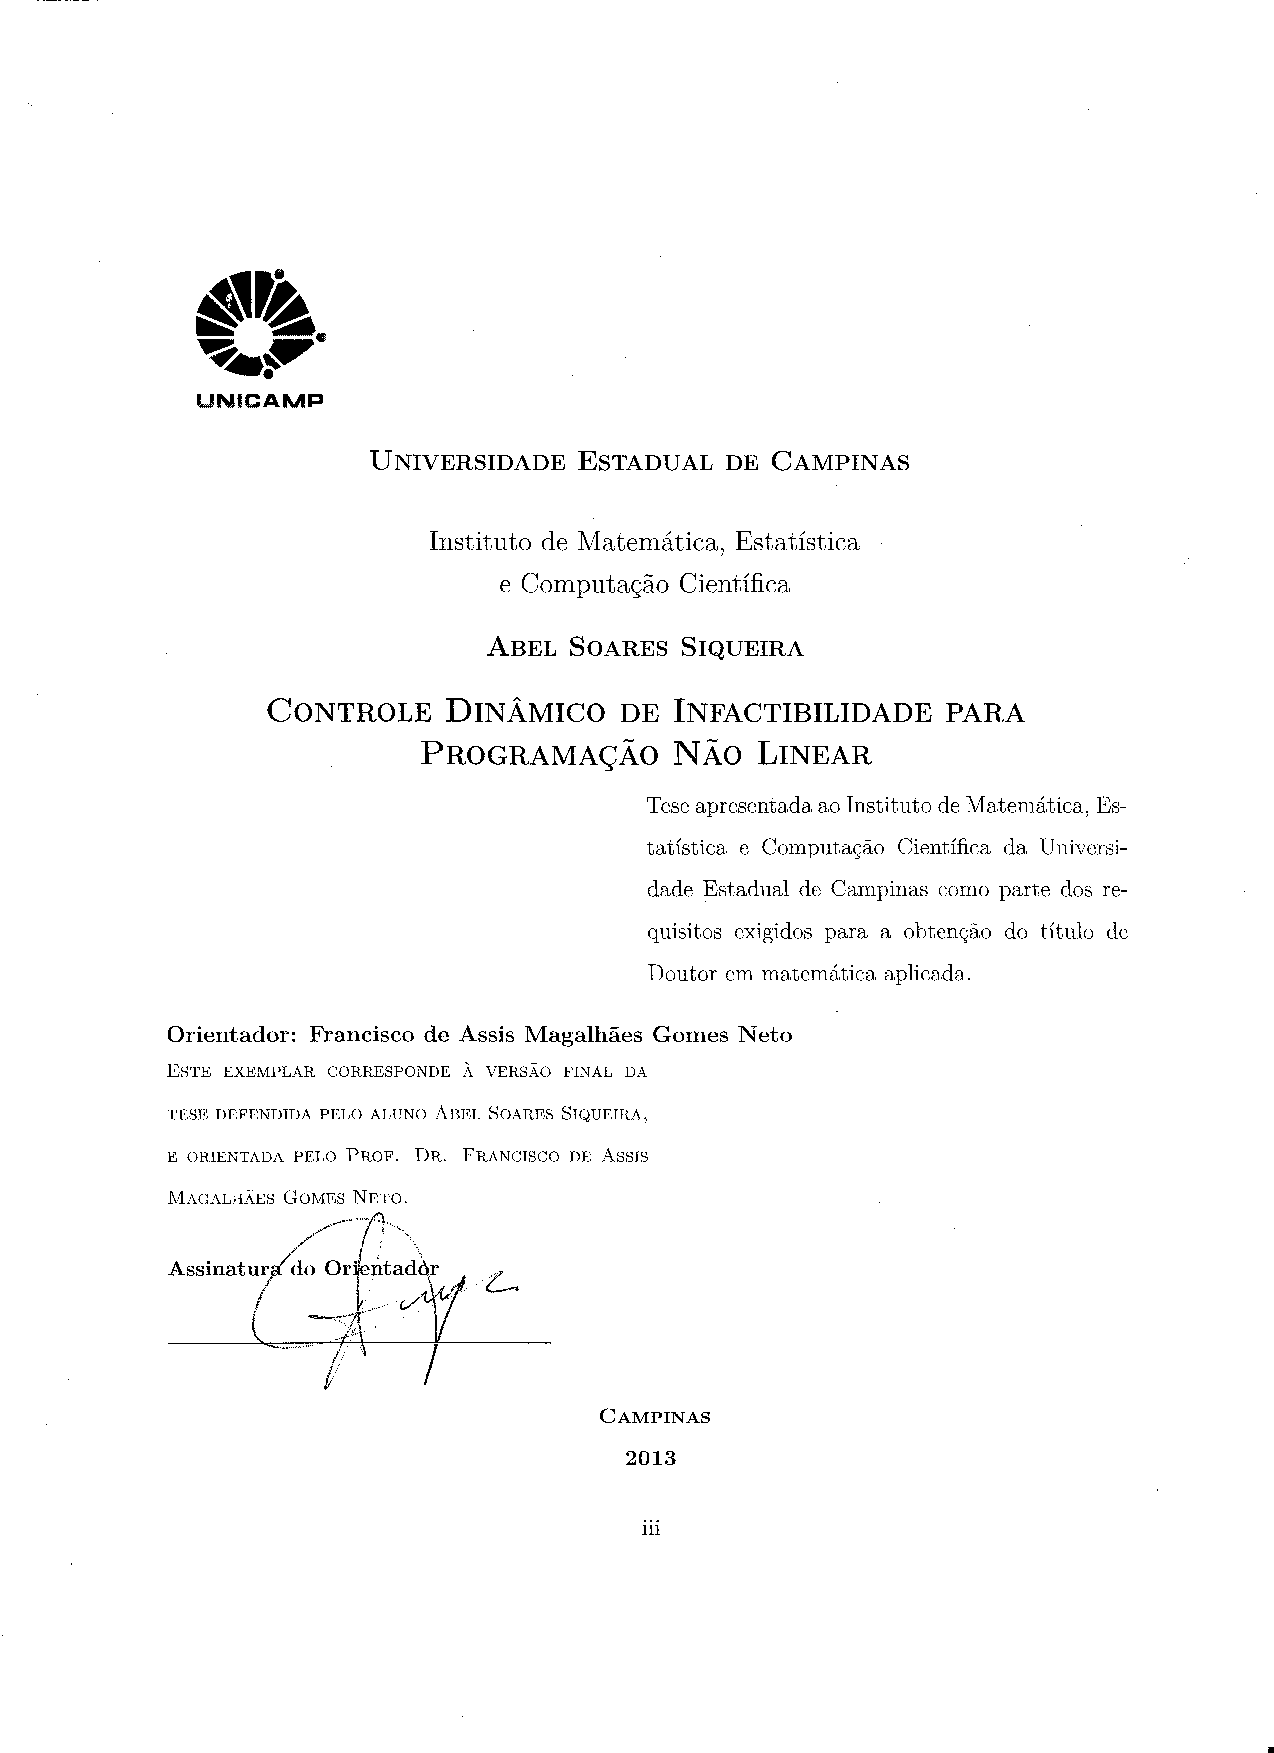
\includepdf[fitpaper=true]{pdfimgs/folha-de-rosto}
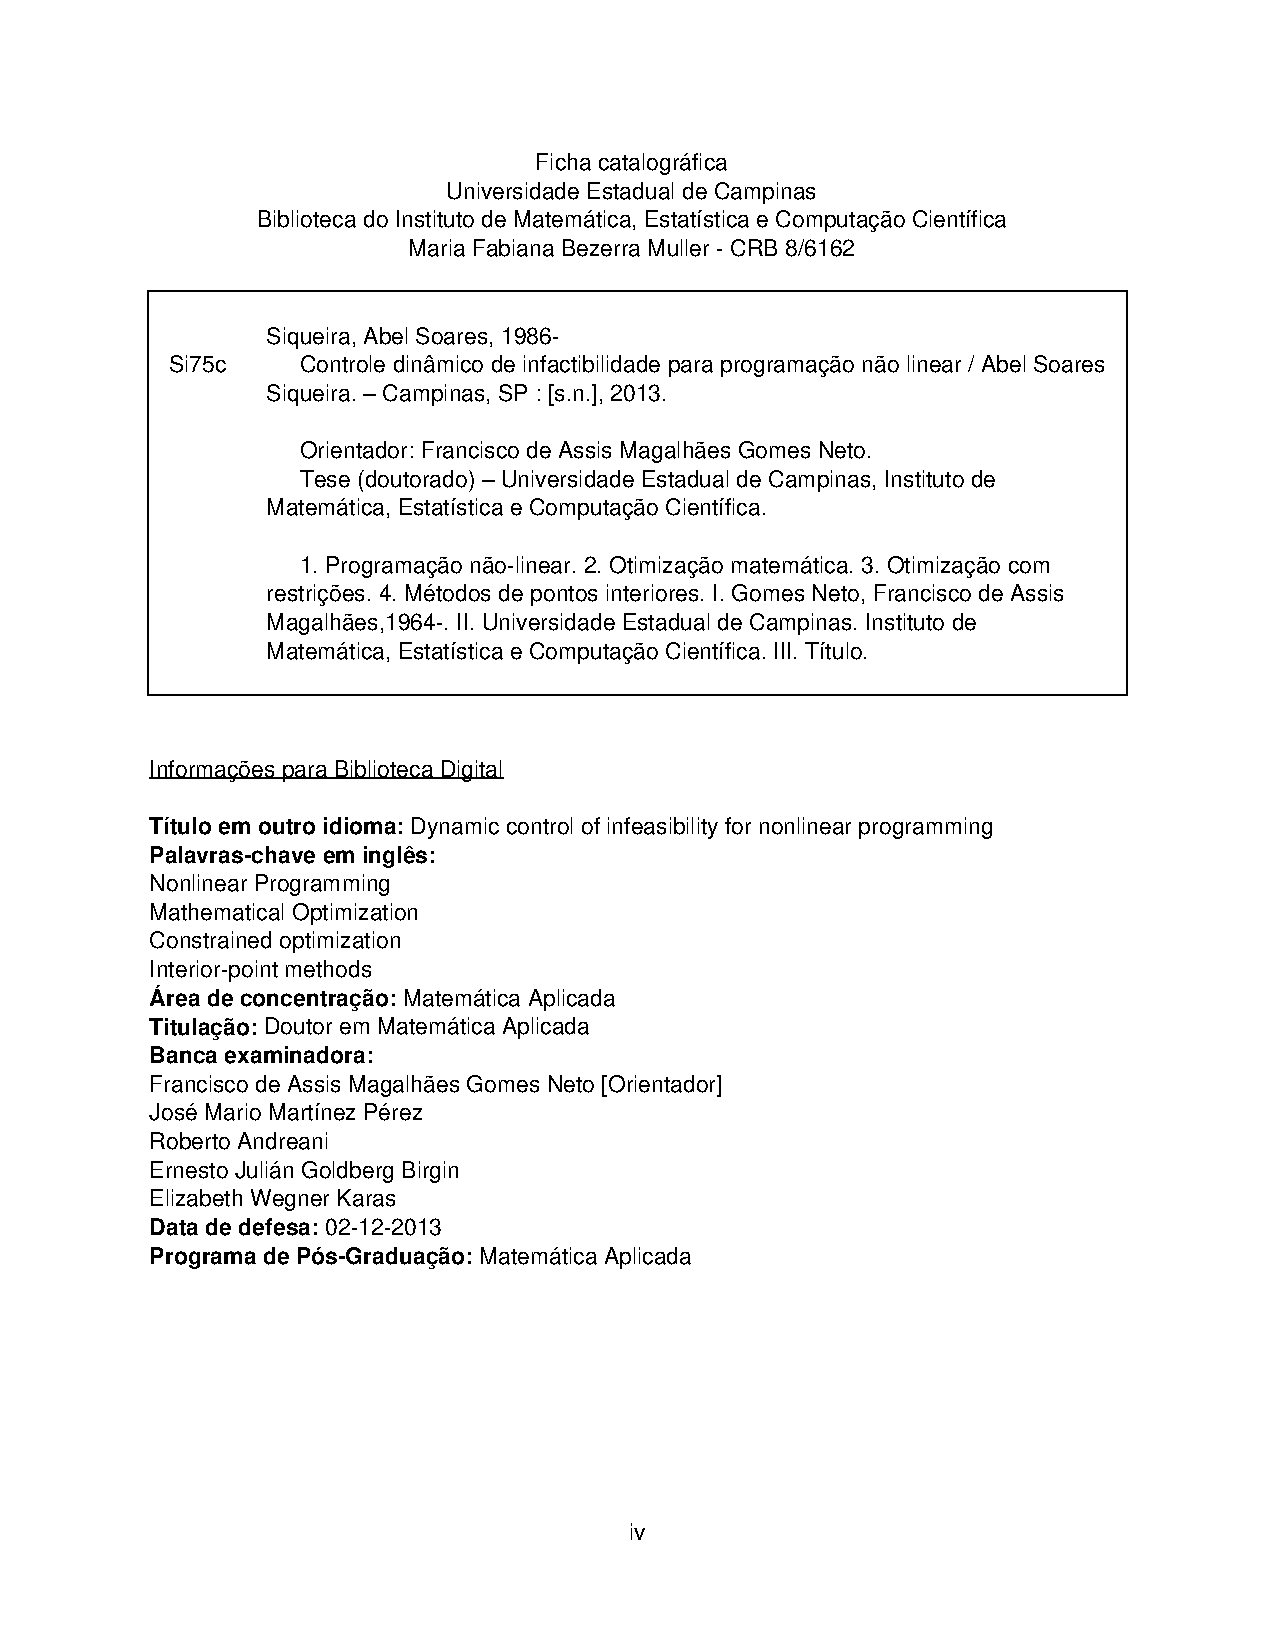
\includepdf[fitpaper=true]{pdfimgs/ficha-catalografica}
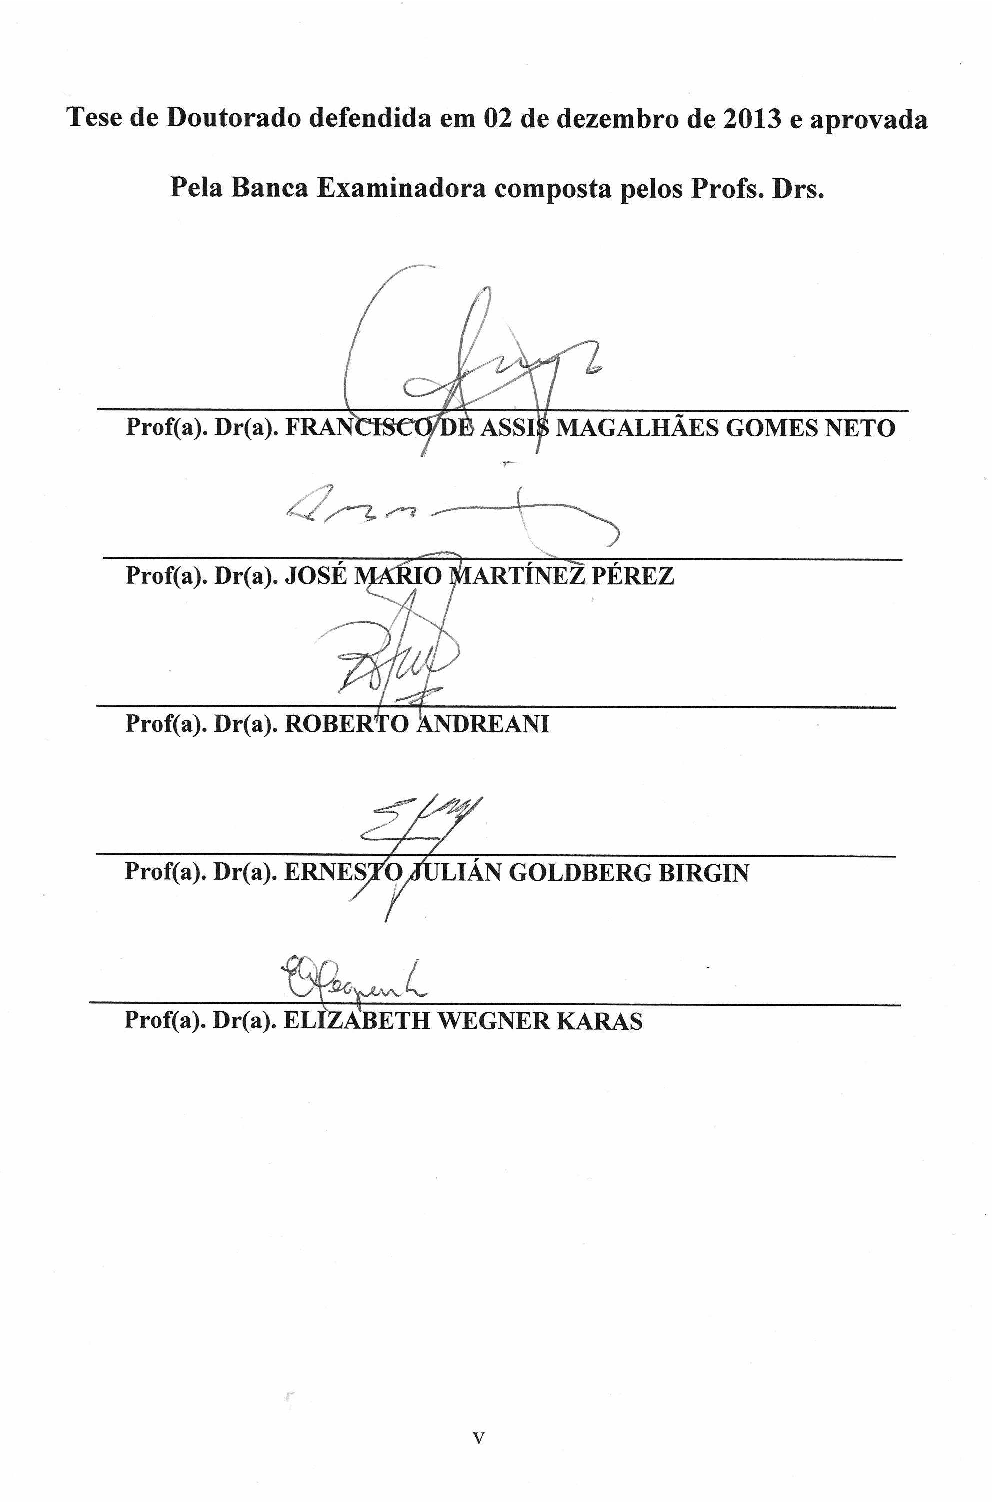
\includepdf{pdfimgs/folha-de-aprovacao}
\chapter*{}
\begin{center}
  \large{\textbf{Abstract}}
\end{center}

One way to solve general nonlinear programming problems is the composite-step
strategies.  These strategies usually combine a step tangent to the constraints
and a normal step, alternating between reducing the objective function value and
the norm of the infeasibility.  This kind of method requires the control of the
steps or the iterates, in order to prevent one step from destroying
the progress of another. We will present an extension of the Dynamic Control of
Infeasibility method, which utilizes a strategy to control the steps known as
Trust Cylinders. This method was originally designed for problems with equality
contraints
only, and our extension will handle general constraints. We'll show numerical
experiments comparing our method with another composite-step method.

\vspace{.5 cm}
\textbf{Keywords:} Nonlinear Programming, Dynamic Control of Infeasibility,
Composite-step Methods, Numerical Experiments.

\vspace{.1\textheight}
\begin{center}
  \large{\textbf{Resumo}}
\end{center}

Uma maneira de resolver problemas gerais de programação não linear é utilizar
estratégias de passos compostos. Essas estratégias normalmente combinam um passo
tangente às restrições e um passo normal, alternando entre a diminuição da função
objetivo e da norma da infactibilidade. Esse tipo de método exige o controle
dos passos ou dos iterandos, para que não se perca o progresso de um passo no outro.
Apresentaremos uma extensão do método de Controle Dinâmico da Infactibilidade, que
utiliza uma estratégia de controle de passos chamado de Cilindros de Confiança.
Esse método foi desenvolvido para problemas com restrições apenas de igualdade,
e nossa extensão lida com restrições gerais. Mostraremos testes numéricos comparando
nosso método com um método do mesmo tipo.

\vspace{.2cm}
\textbf{Palavras-chave } Programação Não-linear, Controle Dinâmico da Infactibilidade,
Métodos de Passos Compostos, Experimentos Numéricos.

\tableofcontents
\chapter*{Agradecimentos\markboth{Agradecimentos}{}}

Aos meus pais, pela educação e apoio toda a minha vida.
Sem eles, nada disso seria capaz. 

À Kally Chung, por estar ao meu lado por todos estes anos, e por
me incentivar nas minhas escolhas.

Ao meu orientador Francisco de Assis, pela sua dedicação ao nosso
trabalho, e por ter sido um ótimo professor desde a minha graduação.

Ao Raniere Gaia pela ajuda com o Linux, e ao Leandro Prudente, pela ajuda com o
Fortran.

Aos meus colegas e amigos, que me ajudaram muito em diversas situações,
especialmente Wanderson Luiz, Douglas Gonçalves e Thadeu Senne.

Ao meus professores, que me deram o conhecimento para chegar até aqui.

À toda minha família, em especial aos meus irmãos.

À Fundação de Amparo à Pesquisa do Estado de São Paulo (Fapesp) pelo apoio
financeiro. (Processo 2009/17273-4)


\mainmatter
\chapter{Introdução}

Vários problemas práticos podem ser formulados como problemas de otimização não
linear. Das várias áreas de engenharia às teorias físicas, muitos problemas
requerem a obtenção de um minimizador ou maximizador. 
Em muitos casos, é possível considerar propriedades específicas do problema e
reduzir a complexidade do modelo, obtendo um problema de otimização com
características especiais, como são os problemas de programação linear, inteira,
quadrática; os problemas de quadrados mínimos, lineares e não lineares; os
problemas convexos, irrestritos; e assim por diante.
No entanto, quando não podemos fazer essa simplificação, é necessário enfrentar
o problema de otimização não linear geral diretamente. Nesta tese, iremos
apresentar um novo método para a solução desse problema.
Nosso método é uma extensão do Método de Controle Dinâmico da
Infactibilidade \cite{bib:chico-dci}, originalmente desenvolvido para o problema
com restrições apenas de igualdade.
O método CDI (do inglês ``Dynamic Control of Infeasibility'') obtém seus
iterandos através de passos normais e tangentes, utilizando aproximações
quadráticas, e técnicas de pontos interiores.
Nossa estratégia de globalização é baseada no que chamamos de \emph{cilindros de
confiança}, que são regiões ao redor do conjunto factível, com raio proporcional
à norma do gradiente projetado.
Esses cilindros limitam a infactibilidade dos iterandos. 
A cada iteração definimos um cilindro pequeno de raio $\rho$ e um cilindro
grande de raio $2\rho$.
Definimos o passo tangente de modo a diminuir o valor da norma do gradiente
projetado, limitando o iterando ao cilindro grande. Prosseguimos então com um ou
mais passos normais, até que o iterando fique dentro do cilindro pequeno. 

Foi preciso decidir como lidar com as desigualdades do problema com cuidado. A
maneira mais direta, considerando o cilindro como uma penalidade das restrições,
não herdava as propriedades do método. 
Escolhemos a estratégia de pontos interiores, e ela se mostrou muito eficaz. A
convergência global do método não teve muitas modificações em relação ao
original com essa estratégia. Para a convergência local, foi preciso considerar
apenas as restrições ativas na solução. Isso gerou algumas mudanças nas
hipóteses e nos teoremas, mas conseguimos obter os mesmos resultados que o
método original.
Uma grande parte deste trabalho foi a implementação do método.
Sempre trabalhamos para suplantar o método original na robustez e na eficiência.
Implementamos nossas estruturas de dados e interfaces tentando aproveitar ao
máximo as ferramentas utilizadas.

Iniciaremos este trabalho com uma revisão do problema de programação não linear,
e de estratégias clássicas no Capítulo \ref{chap:pnl}.
Os detalhes dos
passos tangentes e normais serão mostrados no Capítulo \ref{chap:metodo}, assim
como o pseudo-código para o algoritmo. A teoria de convergência global é
mostrada na seção \ref{sec:conv-global}, e a de convergência local está na seção
\ref{sec:conv-local}. Também vamos falar sobre o comportamento do algoritmo
com problemas infactíveis na Seção \ref{sec:conv-infactivel}. No Capítulo
\ref{chap:implementacao} são mostrados
detalhes da implementação do algoritmo, no Capítulo \ref{chap:resultados}
mostramos os resultados computacionais obtidos com essa implementação, e no
Capítulo \ref{chap:conclusoes} apresentamos nossas considerações finais.

\chapter{Conceitos e Métodos de Programação Não Linear}
\visiblelbl{chap:pnl}

Neste capítulo vamos apresentar alguns conceitos básicos de programação não
linear e analisar alguns métodos tradicionais para o problema geral de
otimização não linear.

\section{Condições de Otimalidade}

Na maior parte deste trabalho, iremos considerar o problema de programação não
linear na forma
\begin{equation}\visiblelbl{prob:geral}
 \begin{array}{rl}
  \min & f(x) \\
   \mbox{suj. a} & c_E(x) =  0, \\
               & c_I(x) \geq 0,
 \end{array}
\end{equation}
com $f:\Rn{n}\to\R$, $c_E:\Rn{n}\to\Rn{m_E}$, $c_I:\Rn{n}\to\Rn{m_I}$
continuamente diferenciáveis até segunda ordem. Definimos $m = m_E+m_I$ e a
função $c:\Rn{n}\to\Rn{m}$, $$ c(x) = \vetor{c_E(x)}{c_I(x)}. $$
A função Lagrangeana para este problema é
\begin{equation}
  \mathcal{L}(x,\lambda) = f(x) + c_E(x)^T\lambda_E + c_I(x)^T\lambda_I = f(x)
    + c(x)^T\lambda,
  \visiblelbl{def:lagrgeral}
\end{equation}
onde $\lambda \in\Rn{m}$ são ditos multiplicadores de Lagrange.
O problema de otimização não linear contínua consiste em encontrar um
minimizador local do problema \eqref{prob:geral}, isto é, um ponto $x^*$ tal que
$f(x^*) \leq f(x)$ para todo $x$ numa vizinhança factível de $x^*$.
\begin{definition}[Regularidade]
  Um ponto viável $x$ é dito regular se os gradientes das restrições ativas em $x$ são
  linearmente independentes, isto é, se o conjunto $\{\nabla c_i(x): c_i(x) =
  0\}$ é linearmente independente.
\end{definition}
Sob a condição de regularidade, podemos mostrar que um minimizador local do
problema dado deve satisfazer as condições abaixo.
\begin{theorem}[KKT]\visiblelbl{teo:kkt}
  Se $x^*$ é um minimizador local do problema \eqref{prob:geral}, então existe
  $\lambda^* \in \Rn{m}$, separado em $\lambda_E^*$ e $\lambda_I^*$, de acordo
  com as igualdades e desigualdades, tal que
  \begin{subequations}\visiblelbl{kkt}
  \begin{align}
    \nabla_x \mathcal{L}(x^*,\lambda^*) = 
    \nabla f(x^*) + \nabla c(x^*)^T\lambda^* & = 0,
      \visiblelbl{kkt.dual} \\
    c_E(x^*) & = 0,
      \visiblelbl{kkt.primaleq} \\
    c_I(x^*) & \geq 0,
      \visiblelbl{kkt.primalineq} \\
    c_{I_i}(x^*)\lambda_{I_i}^* & = 0, \qquad i = 1,\dots,m_I,
      \visiblelbl{kkt.complementarity} \\
    \lambda_I^* & \leq 0.
      \visiblelbl{kkt.negative} 
  \end{align}
  \end{subequations}
  As condições acima são ditas condições de KKT. 
\end{theorem}
A condição \eqref{kkt.dual} é dita factibilidade dual. As condições
\eqref{kkt.primaleq} e \eqref{kkt.primalineq} são ditas factibilidade primal. A
condição \eqref{kkt.complementarity} é dita complementaridade e
\eqref{kkt.negative} é uma condição sobre o sinal dos multiplicadores de
desigualdade.

Vários métodos e estratégias foram criados para tentar resolver o problema
\eqref{prob:geral}.
Apresentaremos agora alguns dos métodos mais tradicionais ou conhecidos, e
vamos ainda comentar sobre estratégias de globalização. Alguns dos métodos
citados resultaram em pacotes computacionais. Quando for possível, iremos
mencionar quais são esses pacotes.

\section{Métodos de Penalização}

Os métodos de penalização definem uma função de medida para infactibilidade, e
procuram resolver o problema irrestrito proveniente da combinação linear da
função objetivo e da penalização.  
Por exemplo, para o problema \eqref{prob:geral}, definimos a função de
penalidade quadrática como
$$ P(x) = \frac{1}{2}\sum_{i=1}^{m_E}c_{E_i}(x)^2 +
\frac{1}{2}\sum_{i=1}^{m_I}\min\{0,c_{I_i}(x)\}^2.$$
Com essa função, definimos o problema irrestrito
\begin{equation*}
  \min \varphi(x,\rho) = f(x) + \rho P(x),
\end{equation*}
onde $\rho$ é um parâmetro real positivo.
Os métodos de penalização tentam minimizar essa função irrestrita, e aumentar
$\rho$ sucessivamente até obter um ponto factível. 
Pode-se mostrar que, dada uma sequência crescente $\{\rho^k\}$ tendendo ao
infinito, e definindo como $x^k$ o minimizador global da função
$\varphi(x,\rho^k)$, a sequência $\{x^k\}$ converge para $x^*$,
minimizador global do problema \eqref{prob:geral}.
Dentre os métodos de penalização, talvez o mais famoso seja o Lagrageano
Aumentado \cite{bib:lagraum}, que define a função de Penalidade como 
\begin{equation*}
  P(x,\lambda) = \frac{1}{2} \sum_{i=1}^{m_E}\bigg[
  c_{E_i}(x)+\frac{\lambda_{E_i}}{\rho}\bigg]^2 +
  \frac{1}{2}\sum_{i=1}^{m_I}\bigg[\min\bigg(0, c_{I_i}(x) +
  \frac{\lambda_{I_i}}{\rho}\bigg)\bigg]^2
\end{equation*}
utilizando o parâmetro $\lambda$, com $\lambda_I\leq 0$, dito multiplicador.
Esse multiplicador é atualizado, usualmente tomando
$$ \lambda_{E_i}^{k+1} = P_{\lambda}(\lambda_{E_i}^k + \rho^k c_{E_i}(x^k)), \qquad 
\lambda_{I_i}^{k+1} = P_{\mu}(\min\{0, \lambda_{I_i}^k + \rho^k c_{I_i}(x^k)\}), $$
onde $P_\lambda$ e $P_\mu$ são as projetores nos intervalos
$[\lambda_\min,\lambda_\max]$ e $[\mu_\min,\mu_\max]$, respectivamente.
Sob certas condições, esses multiplicadores convergem para os Multiplicadores de
Langrange.
Esse método, com uma penalidade deslocada, tem propriedades de convergência
melhores que a penalidade anterior, dita penalidade pura. Algumas implementações
notáveis incluem o pacote LANCELOT, de \citet{bib:lancelot}, e o ALGENCAN, de
\citet{bib:algencan1, bib:algencan2}.

\section{Programação Quadrática Sequencial}

Consideremos o problema com restrições de igualdade
\begin{equation*}
 \begin{array}{rl}
  \min & f(x) \\
   \mbox{suj. a} & c_E(x) =  0.
 \end{array}
\end{equation*}
Uma estratégia para resolver esse problema consiste em fazer aproximações
quadráticas sucessivas da função Lagrangeana, nesse caso definida como
$$ \mathcal{L}(x,\lambda) = f(x) + c_E(x)^T\lambda_E. $$
Uma interpretação para as aproximações quadráticas é a aplicação do Método de
Newton para o sistema não linear
$$ F(x,\lambda) = \nabla\mathcal{L}(x,\lambda) = \vetor{\nabla f(x) + \nabla
c_E(x)^T\lambda}{c_E(x)} = \vetor{0}{0}. $$
A Jacobiana de $F$ é
$$ F'(x,\lambda) = \matriz{\nabla_{xx}^2\mathcal{L}(x,\lambda)} {\nabla
c_E(x)^T} {\nabla c_E(x)} {0}. $$
O Método de Newton a partir do iterando $(x^k,\lambda^k)$ será
$$ \vetor{x^{k+1}}{\lambda^{k+1}} = \vetor{x^k}{\lambda^k} +
\vetor{p_x}{p_{\lambda}}, $$
onde $p_x$ e $p_\lambda$ satisfazem o sistema
$$ \matriz{\nabla_{xx}^2 \mathcal{L}(x^k,\lambda^k)} {\nabla c_E(x^k)^T} {\nabla
c_E(x^k)} {0} \vetor{p_x}{p_\lambda} = \vetor{-\nabla f(x^k) - \nabla
c_E(x^k)^T\lambda^k}{-c_E(x^k)}.$$
Este sistema está relacionado ao problema
\begin{align*}
  \min_p \qquad & \meio p^T\nabla_{xx}^T\mathcal{L}(x^k,\lambda^k) p + \nabla f(x^k)^Tp +
  f(x^k) \\
  \mbox{suj. a} \qquad & \nabla c_E(x^k)p + c_E(x^k) = 0,
\end{align*}
que é a minimização da aproximação quadrática da função $\mathcal{L}(x^k+p_x,\lambda_k)$
com a aproximação linear da restrição $c_E(x^k + p_x) = 0$.
Nesse desenvolvimento, normalmente introduzimos uma região de confiança, de modo
que o problema é reescrito como
\begin{equation}\visiblelbl{prob:sqp}
  \begin{array}{rl}
  \min_p \qquad & \meio p^T\nabla_{xx}^T\mathcal{L}(x^k,\lambda^k) p + 
    \nabla \mathcal{L}(x^k,\lambda_k)^Tp + f(x^k) \\
  \mbox{suj. a} \qquad & \nabla c_E(x^k)p + c_E(x^k) = 0, \\
                    & \norma{p} \leq \Delta.
  \end{array}
\end{equation}
Infelizmente, nem sempre podemos garantir que esse subproblema é factível. Uma
alternativa usada frequentemente
\cite{bib:lalee-implementation, bib:byrd-trust-region, bib:byrd-interior-point,
bib:dennis-convergence-theory, bib:el-alem-1997, bib:el-alem-1999,
bib:chico-nonlinear-programming, bib:chico-gmm99, bib:chico-dci,
bib:curtis-matrix-free, bib:wachter-interior-point}
é a divisão desse passo em dois, normalmente ditos tangente e normal.
O passo tangente normalmente envolve a substituição da restrição do problema
\eqref{prob:sqp} por alguma restrição com garantia de factibilidade.
Uma ideia é calcular passos no espaço tangente dado pela Jacobiana no iterando
atual, representado pelo problema
\begin{align*}
  \min_p \qquad & \meio p^T\nabla_{xx}^T\mathcal{L}(x^k,\lambda^k) p + 
    \nabla \mathcal{L}(x^k,\lambda_k)^Tp + f(x^k) \\
  \mbox{suj. a} \qquad & \nabla c_E(x^k)d = 0, \\
                    & \norma{d} \leq \Delta.
\end{align*}
A partir desse passo, fazemos um passo normal que procura diminuir o valor da 
medida de infactibilidade $\norma{c_E(x)}^2$. 
Outra estratégia é obter primeiro um passo normal, minimizando aproximadamente 
$\norma{c_E(x^k+d)}$, obtendo um passo $d_N$. Daí, tentamos resolver o problema
\begin{align*}
  \min_p \qquad & \meio p^T\nabla_{xx}^T\mathcal{L}(x^k,\lambda^k) p + 
    \nabla \mathcal{L}(x^k,\lambda_k)^Tp + f(x^k) \\
  \mbox{suj. a} \qquad & \nabla c_E(x^k)d = \nabla c_E(x^k)d_N, \\
                    & \norma{d} \leq \Delta.
\end{align*}
Algumas implementações conhecidas são SNOPT, de \citet{bib:snopt}, FILTERSQP,
de \citet{bib:filtersqp}, e o GMM, de
\citet{bib:chico-nonlinear-programming, bib:chico-gmm99}.

\section{Métodos de Restrições Ativas}

A estratégia de Restrições Ativas consiste em separar, a cada iteração, as
restrições que devem ser tratadas como ativas.
Feito isso, o método considera apenas as restrições ativas para
determinar uma direção. 
A ideia provém das condições KKT \eqref{kkt}, que podem ser reescritas como
\begin{align}
  \nabla f(x^*) + \sum_{i\in A}\nabla c_i(x^*)^T\lambda_i^* & = 0, \\
  c_i(x^*) & = 0, \qquad i \in A, \\
  c_i(x^*) & > 0, \qquad i \not\in A, \\
  \lambda_i^* & \leq 0, \qquad i \in A\backslash E, \\
  \lambda_i^* & = 0, \qquad i \not\in A,
\end{align}
onde $A = \{i : c_i(x^*) = 0\} = E\cup\{I_i: c_{I_i} = 0\}$ é o conjunto dos
índices das restrições ativas na solução. Se o conjunto $A$ fosse conhecido a
priori, poderíamos resolver o problema de igualdade
$$ \min f(x) \qquad \mbox{suj. a} \qquad c_i(x) = 0, \qquad i\in A,$$
e a partir da solução deste, obter o valor das outras restrições e dos
multiplicadores adicionais. Se os sinais estiverem corretos, a solução obtida
corresponde à solução do problema original.

A ideia do método consiste então de chutar um conjunto de restrições ativas $A$, e
procurar pela solução do problema com restrições de igualdade correspondente.
Durante o processo, que inicia de um ponto factível, as direções são feitas de
modo a não violar a factibilidade. Caso uma outra restrição seja encontrada no
caminho, ela é incorporada ao conjunto de restrições ativas. Ao encontrar uma
solução, se o sinal dos multiplicadores não estiver correto, o conjunto de
restrições ativas é atualizado retirando a restrição correspondente.

Esse método é muito utilizado para problemas com restrições lineares, devido à
facilidade de se movimentar na superfície gerada pelas restrições ativas. Para
aplicar o método a restrições não lineares, é necessário projetar o passo na
superfície ativa, além de se obter decréscimo suficiente da função objetivo.

\section{Métodos de Pontos Interiores}

Para a estratégia de Pontos Interiores, vamos considerar o problema
\eqref{prob:geral} no formato
\begin{equation*}
 \begin{array}{rl}
  \min & f(x) \\
   \mbox{suj. a} & 
   \begin{array}{rl}
     c_E(x) & =  0, \\
     c_I(x) - s & = 0, \\ 
     s & \geq 0.
   \end{array}
 \end{array}
\end{equation*}
Daqui, definimos o problema de barreira
\begin{equation*}
 \begin{array}{rl}
   \min & f(x) - \mu \displaystyle\sum_{i=1}^{m_I}\ln s_i \\
   \mbox{suj. a} & 
   \begin{array}{rl}
     c_E(x) & =  0, \\
     c_I(x) - s & = 0, \\ 
   \end{array}
 \end{array}
\end{equation*}
onde $\mu > 0$. A condição $s > 0$ fica embutida na função objetivo desse novo
problema. A estratégia de Pontos Interiores consiste em resolver esse problema
aproximadamente, e reduzir gradativamente o parâmetro $\mu$. Espera-se que a
solução quando $\mu\to0$ convirja para a solução do problema original.
Classicamente, o método de Newton é aplicado ao sistema KKT desse subproblema, e
$\mu$ é reduzido seguindo algum esquema de atualização. 
Outra maneira de resolver esse problema é utilizar técnicas de Programação Quadrática
Sequencial ou até mesmo a combinação de penalização para as restrições de
igualdade. Nessa linha destacam-se os trabalhos
\citet{bib:wright-interior, bib:wachter-interior-point, bib:byrd-interior-point,
bib:byrd-trust-region,  bib:ipopt}.
Os pacotes LOQO, de \citet{bib:loqo1,bib:loqo2} e o
IPOPT, de \citet{bib:ipopt, bib:wachter-thesis, bib:wachter-interior-point}, são
algumas implementações tradicionais.

Nosso método utilizará as estratégias de pontos interiores e programação
quadrática sequencial, fazendo a separação dos passos tangente e normal.

\section{Convergência Global}

Os algoritmos de Programação Não Linear precisam de algum controle das
iterações para garantir que o método tenha convergência global, isto é, que gere
uma sequência convergente a um ponto estacionário, ou ao menos com pontos de
acumulação estacionário, partindo de um ponto inicial qualquer.
Existem várias maneiras de se obter convergência global, sendo a maioria
delas alguma extensão ou modificação do uso de busca linear, regiões de
confiança, funções de mérito e filtro. Recomendamos a leitura de
\cite{bib:book-luenberger, bib:book-nocedal, bib:book-conn-trust} para um
aprofundamento nas técnicas. Aqui apresentaremos apenas a ideia básica dessas
estratégias.

Uma maneira de avaliar o progresso do algoritmo é o uso de funções de mérito.
Uma função de mérito é uma função que serve de medida para o progresso do
algoritmo, levando em conta o valor da função objetivo e a infactibilidade do
ponto atual. De um modo geral, podemos escrever uma função de mérito como
$$ \phi(x;\mu) = f(x) + \mu P(x). $$
As escolhas para a função $P$ são, tradicionalmente, as mesmas que as escolhas
para penalização.
Dado um iterando $x^k$ e uma direção de descida $d^k$, fazemos uma busca linear
para encontrar um comprimento de passo $\alpha_k$ tal que $x^{k+1} = x^k +
\alpha_k d^k$
resulta em um decréscimo suficiente para a função.
Uma maneira de fazer essa busca é o chamado \emph{backtracking}, em que se começa
com $\alpha_k = 1$ e reduz-se $\alpha_k$ gradativamente até que alguma
condição de decréscimo é satisfeita.
Uma das condições mais conhecidas é a Condição de Armijo, onde $\alpha_k$ deve
ser tal que
$$ \phi(x^k + \alpha_kd^k;\mu) \leq \phi(x^k;\mu) +
\eta\alpha_k D\phi(x^k;\mu;d^k), $$
onde $\eta\in(0,1)$ e $D\phi(x;\mu;d)$ é a derivada direcional no ponto $x$, na
direção $d$. 

Outra maneira de escolher os passos é a utilização de filtros, uma ideia baseada
em otimização multiobjetivo. Nessa estratégia, também definimos uma função de
medida de infactibilidade, denominada por $P$, e consideramos o problema
\begin{equation}
  \min_x f(x) \qquad \mbox{e} \qquad \min_x P(x). \nonumber
\end{equation}
Esses objetivos são considerados separadamente, e nos interessam os pontos que
conseguem obter alguma melhora em ao menos um dos dois objetivos.
Para cada ponto $x$, definimos um par $(f, P)$, com $f = f(x)$ e $P = P(x)$.
Dizemos que um par $(f_a,P_a)$ domina $(f_b,P_b)$ se $f_a \leq f_b$,
$P_a \leq P_b$, e ao menos uma das desigualdades é estrita.

A estratégia de filtro consiste em manter um conjunto de pontos $\mathcal{F}$,
onde nenhum dos pontos domina outro. Os iterandos são aceitos pela estratégia se
o ponto obtido não é dominado por nenhum dos outros. Nesse caso, ele é
adicionado ao conjunto, e os pontos que ele domina são retirados.
Na prática, é comum utilizar algum decréscimo suficiente para a dominância
também, para evitar que os passos sejam muito pequenos.
A Figura \ref{fig:filtro} representa um possível filtro. Os trabalhos
de \citet*{bib:gonzaga-filter}, \citet*{bib:ribeiro-filter},
\citet*{bib:karas-filter}, e \citet*{bib:pericaro-filter} apresentam métodos com
filtros.
\begin{figure}[!ht]
  \centering
  \begin{tikzpicture}[scale=2.5]
    \draw[->] (-0.2,0) -- (3.2,0) node[right] {$f$};
    \draw[->] (0,-0.2) -- (0,3.2) node[above] {$P$};
    \clip (-0.3,-0.3) rectangle (3.3,3.3);
    \draw[fill] (0.3,2.6) circle (0.02) node[below] {$(f_1,P_1)$};
    \draw[fill] (1,1.2) circle (0.02) node[below] {$(f_0,P_0)$};
    \draw[fill] (2.3,0.7) circle (0.02) node[below] {$(f_2,P_2)$};
    \draw[gray] (0.3,4) -- (0.3,2.6) -- (4,2.6);
    \draw[gray] (1,4) -- (1,1.2) -- (4,1.2);
    \draw[gray] (2.3,4) -- (2.3,0.7) -- (4,0.7);
    \draw[gray,pattern=north west lines, pattern color=gray] (0.3,4) -- (0.3,2.6) --
      (1,2.6) -- (1,1.2) -- (2.3,1.2) -- (2.3,0.7) -- (4,0.7) -- (4,4);
  \end{tikzpicture}
  \caption{Pontos que compõem o filtro. A área hachurada representa a região dos
    pontos dominados}
  \visiblelbl{fig:filtro}
\end{figure}

Outra estratégia é a utilização de regiões de confiança, na qual escolhemos um raio
$\Delta$, e definimos a região $\mathcal{B}_k=\{x:\norma{x-x^k}\leq\Delta\}$, de
modo que a direção de descida $d^k$ satisfaça $x^k+d^k\in\mathcal{B}_k$,
isto é, que $\norma{d^k}\leq\Delta$. 
Em geral, o passo é obtido a partir de um modelo de $\varphi$ em torno de $x^k$,
denotado por $q$. Esse passo é aceito se o decréscimo real da função, em
comparação com o decréscimo previsto pelo modelo, for suficientemente pequeno.
Definimos o decréscimo previsto, Pred, como
$$ \mbox{Pred}(d) = q(0) - q(d), $$
e o decréscimo real, Ared, como
$$ \mbox{Ared}(d) = \phi(x^k;\mu) - \phi(x^k+d;\mu). $$
Em seguida, definimos a razão
$$ \rho^k = \frac{\mbox{Ared}(d^k)}{\mbox{Pred}(d^k)}, $$
e aceitamos ou rejeitamos o passo $d^k$ de acordo com o valor de $\rho^k$.
Por exemplo, se $\rho^k < \frac{1}{4}$, rejeitamos o passo $d^k$, reduzimos
$\Delta$, e calculamos um novo passo. Senão, aceitamos o passo. Se, além disso,
$\rho^k > \frac{3}{4}$, então aumentamos o raio da região de confiança $\Delta$.

O algoritmo apresentado por \citet{bib:chico-dci} define uma nova maneira de se
obter convergência global, chamada de Cilindros de Confiança, que utilizamos
nesta extensão do método.
Com esses cilindros, conseguimos limitar a distância entre os iterandos e o
conjunto factível, e permitir longos passos tangentes.
Os detalhes dessa estratégia serão apresentados no capítulo seguinte.


\chapter{O Método de Controle Dinâmico da Infactibilidade}\visiblelbl{chap:metodo}

O método de Controle Dinâmico da Infactibilidade (CDI) foi desenvolvido originalmente 
para problemas com restrições de igualdade em \cite{bib:chico-dci}. Nosso trabalho estende o algoritmo 
para lidar com inequações e limitantes nas variáveis.
Para desenvolver o algoritmo, nós consideramos o problema no formato
\begin{equation}\visiblelbl{prob:geral_cuter}
\begin{array}{rrrcll}
 \min & f(x) \\
 \mbox{suj. a} & & & c_E(x) & = & 0, \\
& c_L & \leq & c_I(x) & \leq & c_U, \\
& b_L & \leq &     x  & \leq & b_U,
\end{array}
\end{equation}
onde $f:\RnemR{n}$, $c_E:\RnemRn{n}{m_E}$, $c_I:\RnemRn{n}{m_I}$ são continuamente
diferenciáveis até segunda ordem, 
$c_{L_i} \in \R\cup\{-\infty\}, c_{U_i} \in \R\cup\{\infty\}, i = 1,\dots,m_I$, e
$b_{L_i} \in \R\cup\{-\infty\}, b_{U_i} \in \R\cup\{\infty\}, i = 1,\dots,n$.
No entanto, para facilitar o desenvolvimento da teoria do método, 
vamos considerar o problema na forma mais simples, e tradicional, que
apresentamos na seção anterior:
\begin{equation}\tag{\ref{prob:geral}}
 \begin{array}{rl}
  \min & f(x) \\
   \mbox{suj. a} & c_E(x) =  0, \\
               & c_I(x) \geq 0.
 \end{array}
\end{equation}
Introduzindo uma variável de folga $s$ nesse problema, obtemos
\begin{equation}
\begin{array}{rrcl}
 \min & f(x) \\
 \mbox{suj. a} & c_E(x) & = & 0, \\
               & c_I(x) - s & = & 0, \\
               & s & \geq & 0.
\end{array}
\end{equation}
Definindo a vari\'avel
\begin{eqnarray*}
 z = \vetor{x}{s},
\end{eqnarray*}
e a fun\c{c}\~ao
\begin{equation}\visiblelbl{def:h}
h(z) = \vetor{c_E(x)}{c_I(x) - s}, 
\end{equation}
temos o problema com restrições de igualdade e limitantes
\begin{eqnarray*}
  \min & & f(x) \\
  \mbox{suj. a} & & h(z) = 0 \\
       & & s \geq 0.
\end{eqnarray*}

Agora, definimos uma função de barreira $\beta(z)$ que tende ao infinito quando
a variável $z$ se aproxima dos limitantes. No caso, como temos apenas $s\geq 0$,
definimos
\begin{equation}\visiblelbl{def:beta}
\beta(z) = -\sum_{i=1}^{m_I}\ln s_i.
\end{equation}
Discutiremos o caso mais geral para a função de barreira na Seção
\ref{sec:generalizacao}.
Finalmente, definimos a função
\begin{equation}\visiblelbl{def:phi}
  \varphi(z,\mu) = f(x) + \mu\beta(z),
\end{equation}
e obtemos o problema
\begin{equation}\visiblelbl{prob:pto_int}
 \begin{array}{rrcl}
  \min & \varphi(z,\mu) \\
  \mbox{suj. a} & h(z) & = & 0.
 \end{array}
\end{equation}
O Lagrangeano do problema \eqref{prob:pto_int} é dado por
\begin{equation}
 \visiblelbl{def:lagrangeano}
L(z,\lambda,\mu) = \varphi(z,\mu) + \lambda^Th(z).
\end{equation}
Como mencionamos no capítulo anterior, nosso método separa o progresso do
algoritmo em passos tangentes e normais, utilizando aproximações quadráticas da
função Lagrangeana e lineares das restrições.
A ideia por trás de nosso passo tangente é tentar resolver aproximadamente o
problema
\begin{equation}
  \begin{array}{rl}
    \displaystyle\min_{d} & L(z_c + d,\lambda,\mu) \\
    \mbox{suj. a} & h(z_c+d) = h(z_c),
  \end{array}
\end{equation}
onde $z_c$ é o ponto obtido na iteração anterior.
Infelizmente, o problema acima pode ser mal condicionado devido às derivadas da
função objetivo. Isso se deve à presença da inversa da matriz diagonal 
$S = \mbox{diag}(s_1,\dots,s_{m_I})$ nas derivadas de $\varphi$, como mostrado a
seguir:
$$ \nabla_z\varphi(z,\mu) = \nabla_zf(x) + \mu\nabla\beta(z) = 
\vetor{\nabla f(x)}{-\mu S^{-1}e}, $$
$$ \nabla^2_{zz} \varphi(z,\mu) = \nabla_{zz}^2f(x) + \mu\nabla^2\beta(z) = 
\matriz{\nabla^2 f(x)}{0}{0}{\mu S^{-2}}. $$ 
Para facilitar a visualização, vamos omitir o índice $z$
das derivadas quando não houver confusão. Desse modo
$\nabla \varphi(z,\mu) = \nabla_z\varphi(z,\mu)$ 
e $\nabla^2 \varphi(z,\mu) = \nabla^2_{zz}\varphi(z,\mu)$.
Para evitar esse mal condicionamento, vamos
introduzir uma matriz de escalamento $\Lambda(z)$, definida como
$$\Lambda(z) = \matriz{I}{0}{0}{S}.$$
Assim, em nosso passo tangente, fazemos a substituição $d=\Lambda(z_c)\delta$,
melhorando o condicionamento do problema.
Definimos o gradiente, a Hessiana de $\varphi$ e a 
Hessiana do Lagrangeano escalados, respectivamente, como
\begin{eqnarray}
g(z,\mu) & = & \Lambda(z) \nabla\varphi(z,\mu) = \vetor{\nabla f(x)}{-\mu e},
  \visiblelbl{def:gradiente_escalado} \\ 
\Gamma(z,\mu) & = & \Lambda(z) \nabla^2\varphi(z,\mu)\Lambda(z) = 
  \matriz{\nabla^2 f(x)}{0}{0}{\mu I}, \visiblelbl{def:hess_escalada}\\
W(z,\lambda,\mu) & = & \Lambda(z)\nabla_{zz}^2
  L(z,\lambda,\mu)\Lambda(z),\visiblelbl{def:hess_lagr_escalada} \\
& = & \Gamma(z,\mu) + \Lambda(z)\bigg[\sum_{i = 1}^m \lambda_i \nabla^2
 h_i(z)\bigg]\Lambda(z)\nonumber \\
& = & \Gamma(z,\mu) + \sum_{i = 1}^m\lambda_i\matriz{\nabla^2 c_i(x)}{0}{0}{0},
 \nonumber \\
 & = & \matriz{\nabla^2f(x)+\displaystyle\sum_{i=1}^m\lambda_i\nabla^2
   c_i(x)}{0}{0}{\mu I} \nonumber
\end{eqnarray}
onde $m = m_E+m_I$.
Também definimos a Jacobiana escalada como
\begin{eqnarray}
A(z) & = & \nabla h(z) \Lambda(z) = 
\matriz{\nabla  c_E(x)}{0}{\nabla c_I(x)}{-I}\Lambda(z) \nonumber \\
& = & \matriz{\nabla c_E(x)}{0}{\nabla c_I(x)}{-S},
\visiblelbl{def:jacobiana_escalada}
\end{eqnarray}
Nosso método utiliza aproximações para os multiplicadores de Lagrange.
Essas aproximações são feitas a partir da estimativa por quadrados mínimos da
solução da equação de factibilidade dual escalada
$$\Lambda(z) \nabla L(z,\lambda,\mu) = g(z,\mu) + A(z)^T\lambda = 0.$$
Sendo assim, as estimativas são definidas como
\begin{equation}\visiblelbl{lagr:argmin}
\lambda_{LS}(z,\mu) = \arg\min_{\lambda}\bigg\{\meio\norma{A(z)^T\lambda + g(z,\mu)}^2\bigg\}.
\end{equation}
Note que, se $A(z)$ tem posto completo, ent\~ao
$$\lambda_{LS}(z,\mu) = -[A(z)A(z)^T]^{-1}A(z)g(z,\mu).$$
A fatoração da matriz $A(z)A(z)^T$ é feita para calcular os passos internos, de
modo que o custo para encontrar esses multiplicadores não aumenta
consideravelmente o custo total da iteração.

Separando $\lls(z,\mu)$ em 
$$\lls(z,\mu) = \vetor{\lambda_E(z,\mu)}{\lambda_I(z,\mu)},$$ 
$\lambda_E(z,\mu) \in \Rn{m_E}$ e $\lambda_I(z,\mu) \in \Rn{m_I}$,
definimos o gradiente no ponto $z$ projetado no espaço nulo de $A(z)$ escalado
por $\Lambda(z)$ como
\begin{eqnarray}\visiblelbl{gradproj}
 g_p(z,\mu) 
& = & g(z,\mu) + A(z)^T\lambda_{LS}(z,\mu) \\
& = & \Lambda(z) \nabla_zL(z,\lambda_{LS}(z,\mu),\mu) \nonumber \\
& = & \vetor{\nabla f(x) + \nabla c(x)^T \lls(z,\mu)}
 {-\mu e - S\lambda_I(z,\mu)} \visiblelbl{gradproj.vetor}.
\end{eqnarray}
Vamos denotar esta função vetorial como o gradiente projetado.
Na iteração $k$ do algoritmo, calculamos aproximações $\lambda_k$ e $g_p^k$ para
os valores acima. Os detalhes de como são calculadas essas aproximações serão
apresentados na próxima seção.

\section{O Algoritmo CDI}\visiblelbl{sec:algoritmo}

A base do método é o uso do que chamamos de cilindros de confiança.
Esses cilindros são regiões ao redor do conjunto factível, definidas
por
\begin{equation}\visiblelbl{def:cilindro}
 \mathcal{C}(\rho) = \{z \in \Rn{n} : \norma{h(z)} \leq \rho\}.
\end{equation}
O método é dividido em passos normais e tangentes. Os passos
normais servem para aproximar os iterandos da região factível e
os passos tangentes tentam melhorar o progresso dual, segundo uma medida de
otimalidade.
A Figura \ref{fig:cilindro3d} esboça o processo.
\documentclass{standalone}
\usepackage[utf8]{inputenc}
\usepackage[T1]{fontenc}
\usepackage{pgfplots}
\pgfplotsset{compat=1.8}

\newcommand{\norma}[1]{\Vert #1 \Vert}

\begin{document}
\begin{tikzpicture}
  \begin{axis}[view={70}{20}, xmin=-4.4, xmax=3.4, zmin=-1, ymax=-1.8, ymax=1.8,
      axis lines=none,
      xtick=\empty, ytick=\empty, ztick=\empty, x post scale=2.0,
      y post scale=2.5, z post scale=1.1, lightgray
    ]

    \addplot3 [domain=0:360, draw=red!90!white,
      samples=30, samples y=0]
        ({0.3*cos(x)}, {-1.2}, {0.1*1.2*1.2 + 0.3*sin(x)})
        node[pos=0.25, pin=160 : {\color{red}$\norma{h(z)}=\rho^k$}] {};
    \addplot3 [domain=0:360, draw=red!90!white,
      samples=30, samples y=0]
        ({0.6*cos(x)}, {-1.2}, {0.1*1.2*1.2 + 0.6*sin(x)})
        node[pos=0.75, pin=160 : {\color{red}$\norma{h(z)}=2\rho^k$}] {};
    \addplot3 [domain=0:360, draw=red!60!white,
      samples=30, samples y=0]
        ({0.3*cos(x)}, {1.2}, {0.1*1.2*1.2 + 0.3*sin(x)});
    \addplot3 [domain=0:360, draw=red!60!white,
      samples=30, samples y=0]
        ({0.6*cos(x)}, {1.2}, {0.1*1.2*1.2 + 0.6*sin(x)});

    \addplot3[domain=-1.6:1.6, samples y=0, very thick, draw=black]
      ({0}, {x}, {0.1*x^2})
      node [pos=1, below right] {\color{black} $h(z) = 0$};

    \foreach \t in {105,290} {
      \addplot3 [domain=-1.2:1.2,
        draw=red!90!white, samples=30, samples y=0]
        ({0.3*cos(\t)}, {x}, {0.1*x^2 + 0.3*sin(\t)});
       \addplot3 [domain=-1.2:1.2,
        draw=red!90!white, samples=30, samples y=0]
        ({0.6*cos(\t)}, {x}, {0.1*x^2 + 0.6*sin(\t)});
    }

    \addplot3+[solid, draw=blue, mark=*, only marks, mark options={fill=blue}] coordinates {
      (1.1,-0.9,1.0)  (0,-0.95,0.26) (0.1, 1.0, -0.4)
    }
      node [pos=0,above] {\color{black}$z^{k-1}$}
      node [pos=0.35,above left] {\color{black}$z_c^k$}
      node [pos=1,above] {\color{black}$z^k$};
      \node (x0) at (axis cs:1.1,-0.9,1.0) {};
      \node (xc) at (axis cs:0,-0.95,0.26) {};
      \node (x1) at (axis cs:0.1,1.0,-0.4) {};
      \draw[blue,->] (x0) -- (xc);
      \draw[blue,->] (xc) -- (x1);
  \end{axis}
\end{tikzpicture}
\end{document}

Utilizamos como medida de otimalidade a norma do gradiente projetado
aproximado na itera\c{c}\~ao $k$, denotado por $g_p^k$, e 
escolhemos raios dos cilindros de confiança proporcionais a essa medida, isto é,
$$ \rho^k = \bigo(\norma{g_p^k}). $$
Nossas itera\c{c}\~oes devem ser mantidas estritamente fact\'iveis em
rela\c{c}\~ao aos limitantes das vari\'aveis, isto \'e, devemos ter $s >
0$. 
Para garantir isso, dada a direção $d$ a partir de um ponto $z$, calculamos um
tamanho máximo de passo $\alpha$, tal que a nova itera\c{c}\~ao satisfaça
\begin{equation}\visiblelbl{eq:slim}
s + \alpha d_s \geq \epsmu s
\end{equation}
para algum $\epsmu > 0$ pequeno dado, onde $d_s$ é
a componente do vetor $d$ correspondente às variáveis $s$. 
Um esboço do método está descrito no Algoritmo \ref{alg:outline}.
\begin{algorithm}[H]
\caption{Método CDI}
\visiblelbl{alg:outline}
\begin{algorithmic}[1]
\State Parâmetros: $\varepsilon_g > 0$, $\varepsilon_h > 0$, $\varepsilon_a >
0$, $\epsmu \in (0,1)$ e $\nu \in [10^{-4},1]$.
\State Valores Iniciais: $z^0$, $\rho^0 > 0$, $\mu^0$, $k = 1$, $\rhomax^0$.
\State \visiblelbl{alg.step:comeco}Faça a {\bf Etapa Normal}, encontrando $z_c^k$,
  $\lk{k}$, $\rho^k$, $\mu^k$ e $g_p^k = g(z_c^k,\mu^k) + A(z_c^k)^T\lk{k}$
  tais que \visiblelbl{alg:normal-call}
    $$ \norma{h(z_c^k)} \leq \rho^k \leq \nu \frac{\norma{g_p^k}\rhomax^{k-1}}
    {\norma {g(\zc{k},\mu^k)} + 1}, \qquad \mbox{e} \qquad s_c^k \geq \epsmu
    s^{k-1} $$
  \If{ $\norma{h(z_c^k)} < \varepsilon_h$, $\norma{g_p^k} < \varepsilon_g$ e
    $\modulo{(s_c^k)^T\lk{k}} < \varepsilon_a$ }
  \State PARE com $z^* = z_c^k$.
\EndIf
\State Faça a {\bf atualização de $\rhomax^k$}.
\State Faça a {\bf Etapa Tangente}, encontrando $z_k$ com decréscimo suficiente
para a função Lagrangeana e tal que \visiblelbl{alg:tangente-call}
$$ \norma{h(z^k)} \leq 2\rho^k \qquad \mbox{e} \qquad s^k \geq \epsmu s_c^k. $$
\State Incremente $k$ e volte para o passo \ref{alg.step:comeco}.
\end{algorithmic}
\end{algorithm}
A etapa normal do método é composta do cálculo do passo normal e da atualização
dos multiplicadores e do gradiente projetado. 
Os requerimentos sobre o formato desse passo s\~ao poucos, como veremos
posteriormente. Escolhemos encontrar um passo normal com uma sequ\^encia de
itera\c{c}\~oes de algum m\'etodo para resolver o problema 
\begin{equation}\visiblelbl{prob:normal}
\begin{array}{rl}
  \min &\dfrac{1}{2}\norma{h(z)}^2 \\
  \mbox{suj. a} & s \geq 0.
\end{array}
\end{equation}
Nossa estrat\'egia consiste em encontrar um $z_c$ dentro do cilindro de raio 
$\rho$, atualizar o raio, e verificar se $z_c$ permanece dentro do cilindro.
Caso n\~ao permane\c{c}a, repetimos o processo. Cada aplica\c{c}\~ao do m\'etodo
inicia no ponto $z_c$ anterior, sendo que o primeiro $z_c$ da iteração $k$ é
escolhido como $z_c = z^{k-1}$. 
Cada passo que leva a um ponto dentro do cilindro é dito um {\bf passo normal
interno}.
Definimos os subproblemas normais como
\begin{equation}\visiblelbl{prob:normal_direction}
\begin{array}{rl}
  \min & \dfrac{1}{2}\norma{h(z_c+d)}^2 \\
 \mbox{suj. a} & \ell_N \leq d \leq u_N,
\end{array}
\end{equation}
onde 
\begin{equation}\visiblelbl{eq:normal_bounds_definition}
  \ell_N = \vetor{-\Delta_Ne_n}{-\min\{\Delta_Ne_m,(1-\epsmu)s^{k-1}\}}
  \qquad\mbox{e}\qquad u_N = \Delta_Ne_{n+m},
\end{equation}
com $e_n, e_m$ e $e_{n+m}$ são vetores com todas as componentes iguais a $1$, de
tamanho $n$, $m$ e $n+m$, respectivamente.
O Algoritmo \ref{alg:etapa.normal} mostra o esboço da etapa normal.
\begin{algorithm}[H]
\caption{Etapa Normal}
\visiblelbl{alg:etapa.normal}
\begin{algorithmic}[1]
\State Parâmetros: $\alpha_\rho > 0$ e $\alpha_h > 0$.
\State Valores Iniciais: $z_c = z^{k-1}$.
\State Calcule $\lambda$, $g_p = g(z_c,\mu) + A(z_c)^T\lambda$, $\rho$ e
  $\mu$.
\While{ $\norma{h(z_c)} > \rho$ }
  \State Encontre $z_c$ tal que $\norma{h(z_c)} \leq \rho$ e $s_c \geq \epsmu
    s^{k-1}$ pelo {\bf passo normal interno}.
  \State Calcule $\lambda$, $g_p = g(z_c,\mu) + A(z_c)^T\lambda$, $\rho$ e
    $\mu$.
\EndWhile
\State Defina $\lambda^k = \lambda$, $g_p^k = g_p$ e $\rho^k = \rho$.
\State Defina $\mu^k = \min\bigg\{ \mu^{k-1}, \alpha_\rho\rho,
  \alpha_\rho\rho^2, \dfrac{(s_c^k)^T\max\{0,-\lambda_I^k\}}{m_I},
  \alpha_hh(z^k)\bigg\}.$
  \visiblelbl{alg:mudef}
\end{algorithmic}
\end{algorithm}
No algoritmo, calculamos $\lk{k}$ de maneira que fique pr\'oximo a
$\lambda_{LS}(\zc{k} ,\mu^k)$, mas garantimos que o sinal dos multiplicadores
associados \`as desigualdades estejam corretos quando $\mu$ tende a $0$. 
Esse c\'alculo \'e feito como
\begin{equation}\visiblelbl{def:lambda}
  \lambda_i^k = \left\{
    \begin{array}{ll}
      \lambda_{LS_i}(\zc{k},\mu^k), & \mbox{se } i \in E \\ 
      \min\{\lambda_{LS_i}(\zc{k},\mu^k), \alpha(\mu_k)^r\}, & \mbox{se } i \in I \\ 
    \end{array}
  \right.
\end{equation}
onde $\alpha > 0$ e $r > 0$ s\~ao escolhidos adequadamente.
Com esse multiplicador, definimos o gradiente projetado aproximado
$\gpk{k}$ como 
\begin{equation} \visiblelbl{def:gpk}
\gpk{k} = g(\zc{k},\mu^k) + A(\zc{k})^T\lk{k}
= \vetor{ \nabla_x\mathcal{L}(x^k_c, \lk{k}) }
{-\mu^ke - S_c^{k+1}\lk{k}_I},
\end{equation}
de modo que $\gpk{k}$ ficar\'a pr\'oximo
de $g_p(\zc{k},\mu^k).$

A etapa tangente é responsável por diminuir a infactibilidade dual, calculando
um passo tangente que forneça decréscimo suficiente.
O passo é obtido utilizando uma aproximação quadrática para o Lagrangeano e
regiões de confiança, com a direção escalada pela matriz $\Lambda(z_c^k)$. 
Lembramos aqui que, para evitar o mal condicionamento, utilizamos uma aproximação
quadrática de $L(z_c^k + \Lambda(z_c^k)\delta, \lk{k}, \mu^k)$.
Além do decréscimo, o ponto não pode sair do cilindro
$\mathcal{C}(2\rho^k)$.
O passo tangente $\delta_t$ \'e obtido atrav\'es da solu\c{c}\~ao aproximada para o
problema
\begin{equation}\visiblelbl{prob:tangente}
  \begin{array}{rcl}
  \displaystyle\min_{\delta} & & q_k(\delta) = \dfrac{1}{2}\delta^TB^k\delta +
  \delta^Tg_p^k \\
 \mbox{suj. a} & & A(\zc{k})\delta = 0 \\
               & & \ell_T \leq \Lambda(z_c^k)\delta \leq u_T,
  \end{array}
\end{equation}
onde $B^k$ \'e uma aproxima\c{c}\~ao para $W(\zc{k},\lk{k},\mu^k)$, e
os limitantes $\ell_T$ e $u_T$ têm o mesmo formato daqueles definidos
em \eqref{eq:normal_bounds_definition},
mas com uma regi\~ao de confian\c{c}a de raio $\Delta_T$, e $s_c^k$ no lugar de
$s^{k-1}$.
Pedimos que o passo encontrado
seja ao menos melhor que um passo de Cauchy. Então, utilizamos uma implementação
que começa com o passo de Cauchy e tenta melhorar o valor da quadrática, até ser
forçado a parar pelos limitantes, ou ao obter um minimizador da quadrática.
Após o passo tangente, ainda podemos fazer uma correção de segunda ordem, 
conforme sugerido em \cite{bib:book-conn-trust}. Mostraremos como, e quando, é
feita essa correção na Subseção \ref{subsec:soc}.
O ponto obtido pelo passo tangente e pela correção de segunda ordem é o próximo
iterando $z^k$.
O algoritmo \ref{alg:etapa.tangente} mostra um esboço da etapa tangente.
\begin{algorithm}[H]
\caption{Etapa Tangente}
\visiblelbl{alg:etapa.tangente}
\begin{algorithmic}[1]
\State Parâmetros: $\eta_1 \in (0,\meio]$, $\eta_2 > \eta_1$, $\alpha_R \in
(0,\frac{3}{4}]$, $\alpha_I > 1$.
\State Valores Iniciais: $\Delta_T$, $r = 0$ e $z^+ = z_c^k$.
\While{ $\norma{h(z^+)} > 2\rho^k$ ou $r < \eta_1$ }
  \visiblelbl{alg:tangente-condicoes}
  \State Construa $\ell_T$ e $u_T$ usando $\Delta_T$.
  \State Calcule o Passo de Cauchy $\delta_{CP} = -\alpha_{CP}g_p^k$, onde
  $\alpha_{CP}$ é solução de 
    \visiblelbl{alg:cauchy-point}
  \begin{eqnarray*}
    \min_{\alpha > 0} & & q(-\alpha g_p^k) \\
    \mbox{suj. a}  & & \ell_T \leq -\alpha \Lambda(z_c^k) g_p^k \leq u_T.
  \end{eqnarray*}
  \State Calcule um {\bf passo tangente interno} $\delta_t$ tal que
    \visiblelbl{alg:delta-t}
    \begin{eqnarray*}
      q(\delta_t) & \leq & q(\delta_{CP}), \\
      A(z_c^k)\delta_t & = & 0, \\
      \ell_T & \leq & \Lambda(z_c^k)\delta_t \quad \leq \quad u_T.
    \end{eqnarray*}
  \State Se necessário, calcule uma correção de segunda ordem $\dsoc$.
  \State $\dplus = \Lambda(z_c^k) (\delta_t + \dsoc)$.
  \State $z^+ = z_c^k + \dplus$
    \visiblelbl{alg:tangente-plus}
  \State $\Delta L_T^k = L(z^+,\lk{k},\mu^k) - L(z_c^k,\lk{k},\mu^k)$
  \State $r = \dfrac{ \Delta L_T^k }{ q(\delta_t) }$
  \If{ $\norma{h(z^+)} > 2\rho^k$ OU $r < \eta_1$ }
    \State $\Delta_T = \alpha_R\Delta_T$
  \ElsIf{ $r > \eta_2$ }
    \State $\Delta_T = \alpha_I\Delta_T$
  \EndIf
\EndWhile
\State Defina $z^k = z^+$
\end{algorithmic}
\end{algorithm}

Al\'em da norma do gradiente projetado na itera\c{c}\~ao $k$, tamb\'em usamos
a varia\c{c}\~ao do Lagrangeano para controlar o tamanho do raio do cilindro.
Para explicitarmos a contribuição dos passos normal e tangente, dividimos a
variação do Lagrangeano calculado logo após o passo normal em
\begin{equation}\visiblelbl{DLC}
  \Delta \Lc{k} = \Lc{k} - \Lc{k-1} = \DLH{k-1} + \DLV{k},
\end{equation}
onde 
\begin{eqnarray}
  \Lc{k} & = & L(\zc{k},\lk{k},\mu^k), \nonumber \\
 \DLH{k} & = & L(z^k,\lk{k},\mu^k) - L(\zc{k},\lk{k},\mu^k) \visiblelbl{DLH}, \\
 \DLV{k} & = & L(\zc{k},\lk{k}, \mu^k) - L(z^{k-1},\lk{k-1},\mu^{k-1}).
  \visiblelbl{def:DLN}
\end{eqnarray}
A maneira que a atualização de $\rhomax$ é feita está descrita no Algoritmo
\ref{alg:update.rhomax}.
\begin{algorithm}[H]
\caption{Atualização de $\rhomax$}
\visiblelbl{alg:update.rhomax}
\begin{algorithmic}[1]
\State Valores Iniciais: $\Lref$ definido em iterações anteriores.
  Inicialmente $\Lref = \infty$.
\State $\Delta L_N^k = L(z_c^k,\lk{k},\mu^k) - L(z^{k-1},\lk{k-1},\mu^{k-1})$
\If{ $\Delta L_N^k \geq \meio[\Lref - L(z^{k-1},\lk{k-1},\mu^{k-1})]$ }
\visiblelbl{alg:update-rhomax-start}
  \State $\rhomax^k = \rhomax^{k-1}/2$
\Else
  \State $\rhomax^k = \rhomax^{k-1}$
\EndIf
\visiblelbl{alg:update-rhomax-end}
\If{ $\Delta L_N^k > -\meio \Delta L_T^{k-1}$ }
  \visiblelbl{alg:condicao-dlv}
  \State $\Lref = L(\zc{k},\lk{k},\mu^k)$
\EndIf
\end{algorithmic}
\end{algorithm}

\ifdraft
\else
Para deixar mais claro o funcionamento do método, vamos aplicar o algoritmo à
dois exemplos. O primeiro é o problema
\begin{eqnarray}
  \min & f(x) = \meio(x_1^2 + x_2^2) \nonumber \\
  \mbox{s.t} & x_2 = x_1^2 + 1, \nonumber
\end{eqnarray}
cuja solução é o ponto $(1,0)$.

\newcommand{\addexum}[1]{
  \includegraphics[scale=1.0]{ex1_plots/ex1_img#1.pdf}
}

\begin{center}
  \addexum{1}
\end{center}

\begin{center}
  \begin{minipage}{0.9\textwidth}
  Começamos pelo ponto $x_0 = \vetor{2}{3}$, denotado pelo círculo sólido na imagem.
  A curva sólida representa a região factível, as curvas tracejadas 
  denotam o cilindro menor e as curvas pontilhadas denotam o cilindro
  maior. As circunferências concêntricas denotam as curvas de nível da função objetivo, cujo
  menor valor ocorre na origem.
\end{minipage}
\end{center}

\begin{center}
  \addexum{2}
\end{center}

\begin{center}
  \begin{minipage}{0.9\textwidth}
  Iniciamos notando que o ponto não está dentro do cilindro menor. Então
  fazemos um passo normal. O ponto obtido, denotado $x_c$, é a tentativa de
  iterando. Como o ponto já está dentro do cilindro
  menor, o passo é interrompido.
\end{minipage}
\end{center}

\begin{center}
  \addexum{3}
\end{center}

\begin{center}
  \begin{minipage}{0.9\textwidth}
  Agora, atualizamos o raio dos cilindros. Como o $x_c$ obtido continuou
  dentro do cilindro menor após o raio deste ter sido atualizado, definimos
  $x_c^0$ como este iterando normal.
\end{minipage}
\end{center}

\begin{center}
  \addexum{4}
\end{center}

\begin{center}
  \begin{minipage}{0.9\textwidth}
  A partir deste ponto, tentamos realizar um passo tangente. O raio da região de
  confiança, não ilustrado na imagem, é grande o suficiente para permitir que o
  passo seja tomado completamente. O passo aqui é o minimizador da aproximação
  quadrática do Lagrangeano. $x^+$. Nesse caso, como esse ponto está fora do
  cilindro maior, rejeitamos o passo e reduzimos a
  região de confiança.
\end{minipage}
\end{center}

\begin{center}
  \addexum{5}
\end{center}

\begin{center}
  \begin{minipage}{0.9\textwidth}
  Calculamos um novo passo tangente, desta vez limitado pela região de
  confiança, indicada pelo segmento tracejado. Note que, na verdade, este
  segmento faz parte da caixa que é a região de confiança.
  O iterando $x^+$ obtido está dentro do cilindro maior e fornece decréscimo
  suficiente, sendo portanto aceito como o próximo iterando.
\end{minipage}
\end{center}

\begin{center}
  \addexum{6}
\end{center}

\begin{center}
  \begin{minipage}{0.9\textwidth}
  $x^1$ obtido pelo passo tangente.
\end{minipage}
\end{center}

\newpage
Para verificar a aplicação do método no caso com inequações, vamos apresentar
outro exemplo. Note, no entanto, que um problema de duas variáveis e uma
inequação precisaria ser analisado em 3 dimensões. Decidimos, para facilitar a
visualização, mostrar apenas as variáveis originais do problema, e utilizar a
definição da variável de folga para mostrar a restrição deslocada.
Pelo mesmo motivo, vamos mostrar apenas uma parte dos cilindros de confiança.

O problema que consideramos é
\begin{eqnarray}
  \min & f(x) = \meio[x_1^2 + (x_2+1)^2] \nonumber \\
  \mbox{suj. a} & x_2 \geq x_1^2, \nonumber \\
               & x_1 + x_2 = 1, \nonumber
\end{eqnarray}
cuja solução é o ponto $(\frac{-1+\sqrt{5}}{2},\frac{3-\sqrt{5}}{2}) \approx
(0.618,0.382)$.
Ao adicionarmos a variável de folga $s$, obtemos o problema
\begin{eqnarray}
  \min & f(x) = \meio[x_1^2 + (x_2+1)^2] \nonumber \\
  \mbox{suj. a} & x_2 - x_1^2 = s, \nonumber \\
               & x_1 + x_2 = 1, \nonumber \\
               & s \geq 0. \nonumber
\end{eqnarray}
Na solução, o valor de $s$ é $0$.

Os cilindros de confiança para esse problema serão os conjuntos da forma
$$ \mathcal{C}(\rho) = \{(x,s) \in \mathbb{R}^3: (x_2 - x_1^2 - s)^2 +
  (x_1+x_2-1)^2 \leq \rho^2\}. $$
Para mostrar alguma informação dessa região no plano original do problema,
decidimos tomar o caso com $s$ fixo. Dessa maneira, podemos ter alguma
informação do cilindro para as variáveis $x$. Note que essa visualização do
cilindro pode mudar de uma iteração para outra mesmo que o raio do cilindro
permaneça o mesmo.

\newcommand{\addexdois}[1]{
  \includegraphics[scale=1.0]{ex2_plots/ex2_img#1.pdf}
}

\begin{center}
  \addexdois{1}

  $s^0 = 0.01$
\end{center}

\begin{center}
  \begin{minipage}{0.9\textwidth}
    Começamos este exemplo pelo ponto $x^0 = (1,-1)$, e $s^0 = 0.01$, um valor
    pequeno e positivo.
    No gráfico, a reta corresponde à segunda equação; a região hachurada
    correspondente ao conjunto factível da desigualdade; e a parábola sólida
    corresponde à equação $x_2 - x_1^2 = s^0$.
    A curva tracejada denota o corte do cilindro pequeno em $s = s^0$, e a
    pontilhada o corte do cilindro grande pelo mesmo plano.
\end{minipage}
\end{center}

\begin{center}
  \addexdois{2}

  $s_c^0 = 0.01$
\end{center}

\begin{center}
  \begin{minipage}{0.9\textwidth}
    O ponto inicial já está dentro do cilindro pequeno, então o ponto é aceito
    sem necessidade de calcular nenhum passo normal.
  \end{minipage}
\end{center}

\begin{center}
  \addexdois{3}

  $s^+ = 14.15$
\end{center}

\begin{center}
  \begin{minipage}{0.9\textwidth}
    Tentamos agora fazer um passo tangente. O ponto encontrado fica fora do cilindro
    maior e não obtém decréscimo suficiente. Note que o cilindro não é
    visualizado, pois o corte é feito com o valor de $s$ encontrado resulta no
    conjunto vazio. Note que a parábola sólida também não é visualizada por
    causa do valor de $s$.
  \end{minipage}
\end{center}

\begin{center}
  \addexdois{4}

  $s^+ = 3.54$
\end{center}

\begin{center}
  \begin{minipage}{0.9\textwidth}
  O segundo passo tangente obtém decréscimo suficiente e está dentro do cilindro
  maior, que agora pode ser visualizado. Note que a parábola sólida também já
  pode ser visualizada.
\end{minipage}
\end{center}

\begin{center}
  \addexdois{5}

  $s^1 = 3.54$
\end{center}

\begin{center}
  \begin{minipage}{0.9\textwidth}
    O ponto é aceito como iteração tangente.
  \end{minipage}
\end{center}

\begin{center}
  \addexdois{6}

  $s_c = 1.29$
\end{center}

\begin{center}
  \begin{minipage}{0.9\textwidth}
    Atualizamos o raio do cilindro e fazemos um passo normal, levando o ponto
    para dentro do cilindro menor.
  \end{minipage}
\end{center}

\begin{center}
  \addexdois{7}

  $s_c^2 = 1.29$
\end{center}

\begin{center}
  \begin{minipage}{0.9\textwidth}
    Atualizamos novamente o raio do cilindro e o ponto encontrado permance dentro do
    cilindro menor. Portanto encerramos o passo normal.
  \end{minipage}
\end{center}

\begin{center}
  \addexdois{8}

  $s^+ = 1.03$
\end{center}

\begin{center}
  \begin{minipage}{0.9\textwidth}
    Fazemos um passo tangente, que fica dentro do cilindro e também tem
    decréscimo suficiente.
\end{minipage}
\end{center}

\begin{center}
  \addexdois{9}

  $s^2 = 1.03$
\end{center}

\begin{center}
  \begin{minipage}{0.9\textwidth}
    Aceitamos o ponto.
  \end{minipage}
\end{center}

\begin{center}
  \addexdois{10}

  $s_c = 0.67$
\end{center}

\begin{center}
  \begin{minipage}{0.9\textwidth}
    Fazemos um passo normal.
  \end{minipage}
\end{center}

\begin{center}
  \addexdois{11}

  $s_c^3 = 0.67$
\end{center}

\begin{center}
  \begin{minipage}{0.9\textwidth}
    Aceitamos a iteração normal.
  \end{minipage}
\end{center}

\begin{center}
  \addexdois{12}

  $s^+ = 0.16$
\end{center}

\begin{center}
  \begin{minipage}{0.9\textwidth}
    Fazemos um passo tangente.
  \end{minipage}
\end{center}

\begin{center}
  \addexdois{13}

  $s^3 = 0.16$
\end{center}

\begin{center}
  \begin{minipage}{0.9\textwidth}
    Aceitamos a iteração tangente.
  \end{minipage}
\end{center}

\begin{center}
  \addexdois{14}

  $s_c = 0.06$
\end{center}

\begin{center}
  \begin{minipage}{0.9\textwidth}
    Fazemos um passo normal.
  \end{minipage}
\end{center}

\begin{center}
  \addexdois{15}

  $s_c^4 = 0.06$
\end{center}

\begin{center}
  \begin{minipage}{0.9\textwidth}
    Aceitamos a iteração normal. O algoritmo oscila mais algumas iterações ao
    redor da solução até chegar à precisão necessária para declarar
    convergência.
  \end{minipage}
\end{center}


\fi

%A Figura \ref{flux:outline} mostra um fluxograma do método. Por sua vez, as
%figuras \ref{flux:normal} e \ref{flux:tangent} detalham o passo normal e o 
%passo tangente, respectivamente.
%\begin{figure}[H]
%  \centering
%  \begin{tikzpicture}
%    \node[block] (normal) {Encontre $z_c^k$ do {\bf Passo Normal}};
%    \node[decision,below of=normal,node distance=6em] (opt) {O critério de
%      parada é satisfeito?};
%    \node[block,below of=opt,node distance=7em,text width=9em] (end) {FIM.
%    Retorne sucesso com $x^* = x_c^k$.};
%    \node[block,right of=opt,node distance=17em] (tangent) {Encontre $z^k$
%      através do {\bf Passo Tangente}};
%    \node[block,above of=tangent,node distance=6em,text width=7em] (kpp) {$k = k + 1$};
%
%    \algstart{normal}
%    \path[line] (normal) -- (opt);
%    \path[line] (opt) --node[right]{SIM} (end);
%    \path[line] (opt) --node[above]{NÃO} (tangent);
%    \path[line] (tangent) -- (kpp);
%    \path[line] (kpp) -- (normal);
%  \end{tikzpicture}
%  \caption{Esboço do Método}
%  \label{flux:outline}
%\end{figure}
%\begin{figure}[H]
%  \centering
%  \begin{tikzpicture}
%    \node[block] (update) {Atualize $\lambda$, $g_p$};
%    \node[block,below of=update,node distance=5em] (updaterho) {Atualize $\rho =
%      \bigo(\norma{g_p})$};
%    \node[decision,below of=updaterho,node distance=6em] (feasible)
%      {$z_c\in\mathcal{C}(\rho)$?};
%    \node[block,below of=feasible,node distance=7em] (find) {Encontre
%      $z_c\in\mathcal{C}(\rho)$ a partir de \eqref{prob:normal_direction}};
%    \node[block,right of=feasible,node distance=16em] (end) {FIM do {\bf Passo Normal}};
%
%    \algstart[Comece com $z_c = z^{k-1}$]{update}
%    \path[line] (update) -- (updaterho);
%    \path[line] (updaterho) -- (feasible);
%    \path[line] (feasible) --node[right]{NÃO} (find);
%    \path[line] (feasible) --node[above]{SIM} (end);
%    \path[line] (find) -| (-4,0) |- (update);
%  \end{tikzpicture}
%  \caption{Esboço do Passo Normal}
%  \label{flux:normal}
%\end{figure}
%\begin{figure}[H]
%  \centering
%  \begin{tikzpicture}
%    \node[block] (delta) {Encontre $\delta_t$ a partir de \eqref{prob:tangente}};
%    \node[decision,below of=delta,node distance=8.5em] (feasible) {$z_c^k + \delta_t\in
%      \mathcal{C}(2\rho)$ e fornece decréscimo suficiente?};
%    \node[block,below of=feasible,node distance=8.5em, text width=6cm] (soc) {Se necessário,
%      calcule uma correção de segunda ordem $\dsoc$. Caso contrário, $\dsoc = 0$};
%    \node[block,below of=soc,node distance=5.5em, text width=6cm] (accept) {$z^k =
%    z_c^k+\Lambda(z_c^k)(\delta_t+\dsoc)$ e fim do {\bf Passo Tangente}};
%    \node[block,left of=feasible,node distance=16em,text width=6em] (reduce) {Reduza $\Delta_T$};
%    \algstart{delta};
%
%    \path[line] (delta) -- (feasible);
%    \path[line] (feasible) --node[right] {SIM} (soc);
%    \path[line] (feasible) --node[above] {NÃO} (reduce);
%    \path[line] (soc) -- (accept);
%    \path[line] (reduce) |- (delta);
%  \end{tikzpicture}
%  \caption{Esboço do Passo Tangente}
%  \label{flux:tangent}
%\end{figure}
%
%\subsection{O Pseudo-Código}
%
%No Algoritmo \ref{alg:outline} apresentamos o método com mais detalhes.
%Alguns detalhes de implementação serão mostrados no Capítulo
%\ref{chap:implementacao}.
%\begin{algorithm}[H]
%\caption{Método CDI}
%\visiblelbl{alg:outline}
%\begin{algorithmic}[1]
%\State Parâmetros: 
%$\eta_1\in(0,\meio], 
%\eta_2 > \eta_1$,
%$\varepsilon_g$, $\varepsilon_h$, $\varepsilon_a$,
%$\varepsilon_{\mu} > 0$, 
%$\alpha_R \in (0,\frac{3}{4}],
%\alpha_I > 1$,
%$\nu \in [10^{-4}, 1]$.
%\State Valores Iniciais: $z^0$, 
%$\rho^0$, $\rhomax^0$, 
%$\mu^0 > 1$, $\Lref = \infty$,
%$k = 0$
%\State Faça $g_p^0 = g(z^0,\mu^0) + A(z^0)^T\lambda^0$
%\While{ $\norma{g_p^k} > \varepsilon_g$ ou $\norma{h(z^k)} > \varepsilon_h$ ou
%$(s^k)^T\lambda_I^k > \varepsilon_{a}$ }
%  \State $k=k+1$
%  \State $z_c = z^{k-1}$, $\rho = \rho^{k-1}$, $\mu = \mu^{k-1}$
%  \While{ $\norma{h(z_c)} > \rho$ } \Comment{Passo Normal}
%    \State Encontre um ponto $z_c \in \mathcal{C}(\rho)$ tal que
%    $s_c \geq \epsmu s^{k-1}$. Se não for possível, {\bf interrompa} o algoritmo
%      com falha.
%    \State Calcule $\lambda$ e $g_p$
%    \State Atualize $\rho = \nu \norma{g_p} \rhomax/(\norma{g}+1)$
%    \visiblelbl{alg:update-rho}
%  \EndWhile
%  \State Faça $\lambda^k= \lambda$, $g_p^k= g_p$, $\rho^k = \rho$, 
%  \State Faça $\mu^k = \min\bigg\{ \mu^{k-1}, \alpha_{\rho}\rho,
%    \alpha_{\rho}\rho^2, \dfrac{(s_c^k)^T\max\{0,-\lambda^k_I\}}{m_I}, 
%    \alpha_h h(z^k)\bigg\}$.\visiblelbl{alg:mudef}
%  
%  \State $\Delta L_N^k = L(\zc{k}, \lambda^k, \mu^k) -
%    L(z^{k-1}, \lambda^{k-1}, \mu^{k-1})$ 
%    \Comment{Atualização do $\rhomax$}
%  \If{$\Delta L_N^k \geq \meio[\Lref - L(z^{k-1}, \lambda^{k-1}, \mu^{k-1})]$}
%\visiblelbl{alg:condicao-lref}
%    \State $\rhomax^k = \rhomax^{k-1}/2$  
%  \Else
%    \State $\rhomax^k = \rhomax^{k-1}$  
%  \EndIf
%  \If{ $\Delta L_N^k > -\meio\Delta L_T^{k-1}$ } \visiblelbl{alg:condicao-dlv}
%    \State $\Lref = L(\zc{k}, \lambda^k, \mu^k)$
%  \EndIf
%  \State Defina $r = 0$ e $\zp = z_c^k$
%  \Comment{Passo Tangente}
%  \While{ $\norma{h(\zp)} > 2\rho^k$ ou $r < \eta_1$ } \visiblelbl{alg:tangente-condicoes}
%    \State Calcule o Passo de Cauchy $\delta_{CP} = -\alpha g_p^k$, em que
%    $\alpha$ é a solução de
%    \visiblelbl{alg:cauchy-point}
%\begin{eqnarray*}
% \min & & q(-\alpha \gpk{k}) \\
%\mbox{suj. a} & & \norma{\alpha \gpk{k}} \leq \Delta_T, \quad \alpha \geq 0, \\
%& & s_c - \alpha S_c g_{p_s}^k \geq \epsmu s_c
%\end{eqnarray*}
%  \algstore{outline2}
%\end{algorithmic}
%\end{algorithm}
%\begin{algorithm}[H]
%  \caption*{Continuação do Algoritmo \ref{alg:outline}}
%\begin{algorithmic}
%  \algrestore{outline2}
%    \State Calcule um Passo Tangente Interno $\delta_t$, tal que \visiblelbl{alg:delta-t}
%\begin{eqnarray*}
%  q(\delta_t) & \leq & q(\delta_{CP}) \\
%  \norma{\delta_t} & \leq & \Delta_T \\
%  A(z_c^k)\delta_t & = & 0 \\
%  s_c + S_c\delta_{t_s} & \geq & \epsmu s_c
%\end{eqnarray*}
%    \State Se necessário, calcule uma correção de segunda ordem $\dsoc$.
%    \State $\delta_+ = \Lambda(z_c^k)(\delta_t + \dsoc)$.
%    \State $z_+ = \zc{k} + \delta_+$.\visiblelbl{alg:tangente-plus}
%    \State $\Delta L_T^k = L(z_+,\lambda^k, \mu^k) - 
%L(\zc{k},\lk{k}, \mu^k)$
%    \State $r = \dfrac{\Delta L_T^k}{q(\delta_t)}$
%    \If{ $\norma{h(z_+)} > 2\rho$ OU $r < \eta_1$ }
%      \State $\Delta_T = \alpha_R\Delta_T$
%    \ElsIf{ $r > \eta_2$ }
%      \State $\Delta_T = \alpha_I\Delta_T$
%    \EndIf
%  \EndWhile
%  \State Faça $z^k = z_+$
%  \State Escolha $\Delta_T > \Delta_{\min}$.
%\EndWhile
%\end{algorithmic}
%\end{algorithm}





\chapter{Convergência}\label{chap:teoria}

Apresentaremos agora os resultados de convergência do método. Inicialmente
mostraremos que, com condições pouco restritivas, a sequência gerada pelo método
converge para um ponto estacionário. A seguir, mostraremos que, numa vizinhança
do ponto estacionário, se este for um minimizador sob condições satisfatórias, o
método converge superlinearmente em dois passos. Não obstante, mostraremos ainda
que o método converge para pontos estacionários do problema de infactibilidade, de
modo que, se o problema for infactível, não ficará iterando infinitamente.
Foi possível aproveitar todas as propriedades de convergência do método
original \cite{bib:chico-dci}, sendo necessário apenas alguns ajustes para o caso geral com
desigualdades. Para a convergência global, precisamos apenas de algumas
modificações para incluir o parâmetro de barreira. Para a convergência local,
precisamos modificar um pouco os teoremas para tratar apenas das restrições
ativas na solução. 

\section{Converg\^encia Global}\visiblelbl{sec:conv-global}

Apresentamos aqui os resultados de convergência global do método. Veremos que,
com condições relativamente fracas, podemos obter resultados satisfatórios de
convergência. A seguir estão as nossas hipóteses para a prova de convergência do
Algoritmo \ref{alg:outline}.
\begin{hypoenv}\visiblelbl{hip:global.continuidade} 
  As funções $f$, $c_E$ e $c_I$ s\~ao
$C^2$.  
\end{hypoenv} 
\begin{hypoenv}\visiblelbl{hip:global.seq.limitadas} 
  As sequ\^encias $\{\zc{k}\}$ e $\{z^k\}$, as aproxima\c{c}\~oes $B^k$ e os
  multiplicadores $\{\lk{k}\}$ permanecem uniformemente limitados.
\end{hypoenv} 
\begin{hypoenv}\visiblelbl{hip:global.regularidade} A
  restaura\c{c}\~ao n\~ao falha, no sentido de que o algoritmo normal sempre
  encontra um ponto dentro do cilindro, e $\mathcal{Z} = \{\zc{k}\}$ permanece
  longe do conjunto singular de $h$, no sentido que $h$ \'e regular no fecho de
  $\mathcal{Z}$.  Al\'em disso, se a sequ\^encia gerada $\{\zc{k}\}$ \'e
  infinita, ent\~ao 
\begin{equation}\visiblelbl{nnormal} 
  \norma{\zc{k+1}-z^k} = \bigo(\norma{h(z^k)}).
\end{equation} 
\end{hypoenv}
\begin{hypoenv}\visiblelbl{hip:global.dsoc} 
  $\norma{\dsoc^k} = \bigo(\norma{\delta_t^k}^2)$ 
\end{hypoenv} 
A Hipótese \ref{hip:global.continuidade} é natural e esperada, já que canônica,
considerando que, no método, utilizamos essas derivadas, ou aproximações para as
mesmas. 
A Hipótese \ref{hip:global.seq.limitadas} é necessária pois podemos tomar alguma
direção de descida ilimitada. 
As aproximações podem ser definidas de modo a permanecerem
uniformemente limitadas. 
A Hipótese \ref{hip:global.regularidade} é importante pois a restauração pode
falhar. Note que na Seção \ref{sec:conv-infactivel} comentamos sobre a
convergência do método para pontos estacionários da infactibilidade.
A Hipótese \ref{hip:global.dsoc} é tradicional para os passos de correção de
segunda ordem.

Apresentamos agora algumas propriedades provenientes do algoritmo.
Começamos por aquelas relacionadas aos cilindros.
Pela maneira que calculamos os raios dos cilindros no passo
\ref{alg:normal-call} do Algoritmo \ref{alg:outline}, pelas condições dos
iterandos nos passos \ref{alg:normal-call} e \ref{alg:tangente-call} do Algoritmo
\ref{alg:outline}, e pela maneira que atualizamos $\rhomax$ nos passos
\ref{alg:update-rhomax-start}-\ref{alg:update-rhomax-end} do Algoritmo
\ref{alg:update.rhomax}, temos
\begin{eqnarray}
  \rho^k \quad \leq & \rhomax^{k-1}\norma{g_p^k} & \leq \quad
    2\rhomax^k\norma{g_p^k} \visiblelbl{limrho}, \\
  \rhomax^k \quad \leq & \rhomax^{k-1} & \leq \quad
    10^4\rho^k\frac{\norma{g(\zc{k},\mu^k)} + 1} {\norma{\gpk{k}}},
    \visiblelbl{limrhomax} \\
  \norma{h(\zc{k})} \quad \leq & \norma{h(z^{k-1})} & \leq \quad 2\rho^{k-1}.
    \visiblelbl{limhhornormal}
\end{eqnarray}
Como indicado previamente em \eqref{eq:slim} e visto no algoritmo, nossas
iterações seguem uma regra de fração-para-a-fronteira, de modo que são válidas
as inequações
\begin{eqnarray}\visiblelbl{zbound}
 \begin{array}{rcl}
  s_c^{k} & \geq & \epsmu s^{k-1}, \\
  s^{k} & \geq & \epsmu s_c^{k}, \\
  s^+ & \geq & \epsmu s_c^k.
 \end{array}
\end{eqnarray}
Alem disso, pela definição de $\mu^k$ no passo \ref{alg:mudef} do Algoritmo
\ref{alg:etapa.normal}, temos
\begin{equation}\visiblelbl{limmu}
  \mu^k \leq \alpha_{\rho}\min\{\rho^k,(\rho^k)^2\}.
\end{equation}
Deste ponto em diante, supomos que as sequências $\{\zc{k}\}$ e $\{z^k\}$,
geradas pelo algoritmo, satisfazem
\ref{hip:global.continuidade}-\ref{hip:global.dsoc}. Denotando por $\delta_N^k$
o passo normal e por $\delta_T^k$ o passo tangente na iteração $k$, temos
\begin{equation*} \delta_N^k = z_c^k - z^{k-1} \qquad \mbox{e} \qquad \delta_T^k
= z^k - \zc{k} = \delta_t^k + \dsoc^k.  \end{equation*} As hipóteses
\ref{hip:global.continuidade}-\ref{hip:global.dsoc} nos permitem escolher uma
constante $\dmax > 0$, tal que, para todo $k$,
\begin{equation}\visiblelbl{limdmax} 
  \norma{\delta_t^k} + \norma{\dsoc^k} + \norma{\delta_N^k} \leq \dmax.  
\end{equation} As
hipóteses tamb\'em nos permitem definir $\xi_0 > 0$, tal que, $\forall k$, se
$\norma{z - \zc{k}} \leq \dmax$ e $\mu \leq \mu_{0}$, ent\~ao 
\begin{eqnarray}
  \norma{A_j(z)} & \leq & \xi_0, \qquad j = 1,\dots,m \visiblelbl{limjacob} \\
  \norma{\nabla^2 h_j(z)} & \leq & \xi_0, \qquad j = 1,\dots,m
  \visiblelbl{limhessh} \\
  \norma{\nabla f(x)} & \leq & \xi_0, \visiblelbl{limgrad} \\
  \norma{\nabla^2 f(x)} & \leq & \xi_0, \visiblelbl{limhess} \\
  \norma{g(z,\mu)} & \leq & \xi_0, \visiblelbl{limgamma} \\
  \norma{\Gamma(z,\mu)} & \leq & \xi_0, \visiblelbl{limGamma} \\
  \norma{B^k} & \leq & \xi_0, \visiblelbl{limB} \\
  \norma{\lk{k}} & \leq & \xi_0, \visiblelbl{limlambda} \\
  \norma{\dsoc^k} & \leq & \xi_0\norma{\delta_t^k}^2 \visiblelbl{limsoc} \\
  \norma{\Lac{k}} & \leq & \xi_0 \visiblelbl{limLac}, 
\end{eqnarray}
  \begin{eqnarray}\visiblelbl{zcompact}
\begin{array}{rcl} s_c^{k} & \leq & \xi_0 s^{k-1}, \\
  s^k & \leq & \xi_0 s_c^{k}. 
\end{array} 
\end{eqnarray} 
Também supomos que (\ref{nnormal}) pode
ser reescrito como 
\begin{equation}\visiblelbl{nnormalxi} 
  \norma{\zc{k+1} - z^k}
\leq \xi_0\norma{h(z^k)}.  
\end{equation} 
Definimos as matrizes $\Lac{k} = \Lambda(\zc{k})$, $\Lak{k} = \Lambda(z^k)$ e
$\Lambda^+ = \Lambda(\zp)$, para facilitar a notação. 
  Nosso resultado de convergência global é dado no Teorema
  \ref{teo:conv-global}. Esse resultado depende dos próximos cinco lemas. O
  Lema \ref{lemma:31} a seguir dá um limitante para o aumento da infactibilidade
  do causada pelo passo tangente em relação ao iterando obtido no passo normal.

\begin{lemma}\visiblelbl{lemma:31} 
  A tentativa de itera\c{c}\~ao $\zp$ gerada na
  linha \ref{alg:tangente-plus} do Algoritmo \ref{alg:etapa.tangente} satisfaz
  \begin{equation}\visiblelbl{limvarh} 
    \norma{h(\zp) - h(\zc{k})} \leq \bxi_0\norma{\delta_t}^2,
  \end{equation} 
  em que $\barra{\xi}_0$ é uma constante positiva.
\end{lemma} 
\begin{proof} Iremos
  omitir os \'indices $k$ nessa demonstra\c{c}\~ao. A itera\c{c}\~ao \'e
  definida por $\zp = z_c + \dplus = z_c + \Lambda_c(\delta_t + \dsoc)$.  Usando
  uma expansão de Taylor, o fato de que $A_j(z_c)\delta_t = 0$ e
  (\ref{limhessh}), podemos garantir que existe $\zxi^j = \eta_j\zp +
  (1-\eta_j)z_c$, tal que
\begin{eqnarray} 
  \modulo{h_j(\zp) - h_j(z_c)} & = & \modulo{\nabla h_j(z_c)^T\dplus +
    \meio(\dplus)^T\hess h_j(\zxi^j)\dplus} \nonumber \\
  & = & \modulo{\nabla h_j(z_c)^T\Lac{k}(\dt+\dsoc) +
      \meio(\delta_t+\dsoc)^T\Lac{k}\hess h_j(\zxi^j)\Lac{k}(\delta_t +
    \dsoc)} \nonumber \\
  & \leq & \modulo{A_j(z_c)^T(\delta_t+\dsoc)} +
    \meio\norma{\delta_t+\dsoc}^2\norma{\Lac{k}}^2\norma{\hess h_j(\zxi^j)}
    \nonumber \\
  & \leq & \modulo{A_j(z_c)^T\dsoc} + \meio\norma{\delta_t+\dsoc}^2\xi_0^3.
    \label{lemma31.aux}
\end{eqnarray}
Agora, por \eqref{limjacob} e \eqref{limsoc}, temos
$$ \modulo{A_j(z_c)^T\dsoc} \leq \xi_0^2\norma{\delta_t}^2, $$
e pela desigualdade $\norma{v+w}^2 \leq 2(\norma{v}^2 + \norma{w}^2)$,
\eqref{limsoc} e \eqref{limdmax},
$$ \meio\norma{\delta_t + \dsoc}^2 \leq \norma{\delta_t}^2 + \norma{\dsoc}^2
\leq \norma{\delta_t}^2 + \dmax\xi_0\norma{\delta_t}^2. $$
Substituindo essas duas desigualdades em \eqref{lemma31.aux}, obtemos
\begin{eqnarray*}
 \modulo{h_j(\zp) - h_j(z_c)} 
  & \leq & \xi_0^2\norma{\delta_t}^2 + \xi_0^3(\norma{\delta_t}^2 +
    \xi_0\dmax\norma{\delta_t}^2) \\
  & \leq & \xi_0^2(1 + \xi_0 + \xi_0^2\dmax)\norma{\delta_t}^2.
\end{eqnarray*} 
  Definindo $\bxi_0 = \sqrt{m}\xi_0^2(1 + \xi_0 + \xi_0^2\dmax)$, temos o
  resultado desejado.
\end{proof}

O lema a seguir mostra que, se as hipóteses
\ref{hip:global.continuidade}-\ref{hip:global.dsoc} são satisfeitas, o passo
tangente não falha, e obtemos redução suficiente no Lagrangeano.
\begin{lemma}\visiblelbl{lemma:32} Se $x_c^k$ não é um ponto estacionário para o
  problema \eqref{prob:geral}, então $\zp$ \'e aceito com suficientes iterações.
  Al\'em disso,
  podemos definir constantes $\xi_1$, $\xi_2$ e $\xi_3$ tais que, para todo $k$,
\begin{equation}\visiblelbl{limDLHp} \DHp \leq
-\xi_1\norma{\gpk{k}}\min\{\xi_2\norma{\gpk{k}},\xi_3\sqrt{\rho^k},1-\epsmu\}.
\end{equation} \end{lemma} \begin{proof} Iremos omitir os \'indices $k$ nessa
  demonstra\c{c}\~ao. Seja $\zp = z_c + \dplus = z_c + \Lambda_c(\dt + \dsoc)$
  um candidato obtido na linha \ref{alg:tangente-plus} da $k$-\'esima
  itera\c{c}\~ao do Algoritmo \ref{alg:outline}.

  Utilizando uma expans\~ao de Taylor e \eqref{limvarh}, existe $z_\xi = \eta
  z^+ + (1-\eta)z_c$, para algum $\eta\in[0,1]$, tal que
\begin{eqnarray} 
  \DHp & = & L(\zp,\lambda,\mu) - L(z_c,\lambda,\mu) \nonumber \\
   & = & \varphi(\zp,\mu) - \varphi(z_c,\mu) + \lambda^T[h(\zp) - h(z_c)]
  \nonumber \\
  & \leq & \nabla \varphi(z_c,\mu)^T\dplus + \meio(\dplus)^T\hess
  \varphi(\zxi,\mu)\dplus + \xi_0\bxi_0\norma{\dt}^2. \visiblelbl{dlh:passo1}
\end{eqnarray}
Para o primeiro termo, usando \eqref{def:gradiente_escalado}, o fato de que
$g(z_c,\mu)^T\delta_t = (g_p^k)^T\delta_t$, a definição \eqref{prob:tangente},
e as condições \eqref{limsoc}, \eqref{limgamma} e
\eqref{limB}, temos
\begin{align}
  \nabla\varphi(z_c,\mu)^T\delta^+ & = \nabla\varphi(z_c,\mu)^T\Lambda_c
  (\delta_t+\dsoc) \nonumber \\
  & = g(z_c,\mu)^T(\delta_t + \dsoc) \nonumber \\
  & = q(\delta_t) - \meio\delta_t^TB\delta_t + g(z_c,\mu)^T\dsoc \nonumber \\
  & \leq q(\delta_t) + \bigg(\meio\xi_0 + \xi_0^2\bigg)\norma{\delta_t}^2.
  \visiblelbl{dlh:passo2}
\end{align}
Para o segundo termo de \eqref{dlh:passo1}, usando \eqref{def:hess_escalada},
\eqref{limGamma}, \eqref{zbound}, a desigualdade $\norma{v+w}^2 \leq 2(\norma{v}^2
+ \norma{w}^2)$, \eqref{limdmax} e \eqref{limsoc}, temos
\begin{align}
  \meio(\delta^+)^T\nabla^2\varphi(z_\xi,\mu)\delta^+ & =
    \meio(\delta_t+\dsoc)^T\Lambda_c\Lambda(z_{\xi})^{-1}\Gamma(z_{\xi},\mu)
    \Lambda(z_{\xi})^{-1}\Lambda_c(\delta_t + \dsoc) \nonumber \\
  & \leq \dfrac{1}{2}\norma{\Gamma(z_{\xi},\mu)} \norma{\Lambda(z_{\xi})^{-1}
    \Lambda_c}^2 \norma{\delta_t+\dsoc}^2  \nonumber \\
  & \leq \dfrac{1}{2} \dfrac{\xi_0}{\epsmu^2} \norma{\delta_t + \dsoc}^2
    \nonumber \\
  & \leq \frac{\xi_0}{\epsmu^2} (\norma{\delta_t}^2 + \norma{\dsoc}^2) \nonumber
    \\
  & \leq \frac{\xi_0}{\epsmu^2} (1+\xi_0\dmax)\norma{\delta_t}^2.
    \visiblelbl{dlh:passo3}
\end{align}
Assim, substituindo \eqref{dlh:passo2} e \eqref{dlh:passo3} em
\eqref{dlh:passo1}, temos
\begin{align}
  \DHp & \leq q(\delta_t) + \bigg(\frac{\xi_0}{2}+\xi_0^2\bigg)\norma{\delta_t}^2
  + \frac{\xi_0}{\epsmu^2}(1+\xi_0\dmax)\norma{\delta_t}^2
  + \xi_0\barra{\xi_0}\norma{\delta_t}^2 \nonumber \\
  & = q(\delta_t) + \barra{\xi}_1\norma{\delta_t}^2, \visiblelbl{auxdhp}
\end{align} 
onde $\barra{\xi}_1 = \frac{\xi_0}{2} + \xi_0^2 + \frac{\xi_0}{\epsmu^2} (1 +
\xi_0\dmax) + \xi_0\barra{\xi}_0$.

Pela defini\c{c}\~ao de $\dcp$ na linha \ref{alg:cauchy-point} do Algoritmo
\ref{alg:etapa.tangente}, temos $$\norma{\dcp} \geq
\min\left\{\frac{\norma{g_p}}{\norma{B}},\Delta,1-\epsmu \right\} \geq
\min\left\{\frac{\norma{g_p}}{\xi_0}, \Delta, 1 - \epsmu \right\}$$ e
\begin{equation}\visiblelbl{limqdcp} q(\dcp) \leq \meio\dcp^Tg_p \leq
-\meio\norma{g_p}\min\left\{ \frac{\norma{g_p}}{\xi_0}, \Delta, 1 - \epsmu
\right\}.  \end{equation}

Vamos mostrar que $\zp$ \'e aceito se $\Delta \leq \barra{\Delta}$, onde
\begin{equation}\visiblelbl{bdelta} \barra{\Delta} =
\min\left\{\frac{\norma{g_p}}{4\bxi_1}, 1-\epsmu, \sqrt{\frac{\rho}
{\bxi_0}}\right\}.  \end{equation} Note que $\xi_0 < 4\bxi_1$, logo
\begin{equation}\visiblelbl{limbdelta} \barra{\Delta} \leq
\frac{\norma{g_p}}{\xi_0}.  \end{equation} Como $\Delta \leq \barra{\Delta}$,
usando (\ref{limbdelta}), podemos simplificar (\ref{limqdcp}) para
\begin{equation}\visiblelbl{limqdcp2} 
  q(\dcp) \leq -\meio\norma{g_p}\Delta.
\end{equation}
Combinando $\norma{\dt} \leq \Delta$ e $q(\dt) \leq q(\dcp)$ da linha
\ref{alg:delta-t} do Algoritmo \ref{alg:etapa.tangente}, com (\ref{bdelta}) e
(\ref{limqdcp2}) obtemos 
\begin{eqnarray} 
  \bxi_1\norma{\dt}^2 & \leq & \bxi_1\Delta^2 \leq \bxi_1\barra{\Delta}\Delta
  \nonumber \\ 
  & \leq & \frac{1}{4}\norma{g_p}\Delta \leq -\meio q(\dcp) \leq -\meio q(\dt).
\visiblelbl{limxi1} 
\end{eqnarray} 
Agora, de (\ref{auxdhp}) e (\ref{limxi1}),
temos \begin{equation}\visiblelbl{negDHp} \DHp \leq \meio q(\dt) < 0,
\end{equation} de modo que 
\begin{equation}\visiblelbl{rgeqeta1} 
  r = \frac{\DHp}{q(\dt)} \geq \meio \geq \eta_1.  
\end{equation}
Como $\Delta \leq \barra{\Delta}$ e $\norma{h(z_c)} \leq \rho$, usando
(\ref{limvarh}) e (\ref{bdelta}), temos $$\norma{h(\zp)} \leq \rho + \bxi_0
\norma{\dt}^2 \leq \rho + \bxi_0\barra{\Delta}^2 \leq 2 \rho.$$ Portanto, ambas
condi\c{c}\~oes da linha \ref{alg:tangente-condicoes} do Algoritmo
\ref{alg:etapa.tangente} s\~ao satisfeitas e $\zp$ \'e aceito.

Para provar a segunda parte, vamos lembrar que cada vez que o passo \'e
rejeitado, multiplicamos o raio $\Delta$ por $\alpha_R$. Ent\~ao podemos assumir
que o raio aceito satisfaz $\Delta \geq \alpha_R\barra{\Delta}$, onde $0 <
\alpha_R < 1$. Combinando isto com (\ref{negDHp}), a condição $q(\dt) \leq
q(\dcp)$, (\ref{limqdcp}), (\ref{limbdelta}) e (\ref{bdelta}), obtemos 
\begin{eqnarray*}
  \DHp & \leq & \meio q(\dt) \leq \meio q(\dcp) \\ 
   & \leq & -\frac{1}{4}\norma{g_p}\min\left\{ \frac{\norma{g_p}}{\xi_0},
    \Delta, 1 - \epsmu\right\} \\ 
  & \leq & - \frac{1}{4}\norma{g_p}\alpha_R\barra{\Delta} \\ 
  & \leq & -\xi_1\norma{g_p}\min\{\xi_2\norma{g_p}, \xi_3\sqrt{\rho}, 1 -
    \epsmu\}, 
\end{eqnarray*} 
com $\xi_1 = \alpha_R/4$, $\xi_2 = 1/(4\bxi_1)$ e
$\xi_3 = 1/\sqrt{\bxi_0}$.  \end{proof}

O próximo lema define um limitante superior para a variação normal do
Lagrangeano. Note que essa variação pode ser positiva.
\begin{lemma}\visiblelbl{lemma:33} 
  Existe uma constante positiva $\xi_4$ tal que, para $k$ suficientemente
  grande,
  $$\DLV{k+1} \leq \xi_4\rhomax^k\norma{\gpk{k}}.  $$ 
\end{lemma} 
\begin{proof}
    Usando o Teorema do Valor Médio, temos
\begin{eqnarray*} 
    \DLV{k+1} & = & L(\zc{k+1},\lk{k+1},\mu^{k+1}) - L(z^k,\lk{k},\mu^k) \\ 
    & = & \varphi(\zc{k+1},\mu^{k+1}) - \varphi(z^k,\mu^k) + h(\zc{k+1})^T\lk{k+1} -
      h(z^k)^T\lk{k} \\ 
    & = & \varphi(\zc{k+1},\mu^k) - \varphi(z^k,\mu^k) + h(\zc{k+1})^T\lk{k+1} -
      h(z^k)^T\lk{k} + (\mu^{k+1}-\mu^k)\beta(z_c^{k+1}) \\
    & = & \nabla \varphi (\zxi,\mu^k)^T(\zc{k+1}-z^k) + h(\zc{k+1})^T\lk{k+1} -
      h(z^k)^T\lk{k} + (\mu^{k+1}-\mu^k)\beta(z_c^{k+1}) \\
    & =  & \nabla f(x_{\xi})^T(x_c^{k+1}-x^k) +
      \mu^k\nabla\beta(z_{\xi})^T(z_c^{k+1}-z^k) + h(\zc{k+1})^T\lk{k+1} -
      h(z^k)^T\lk{k} \\
    & & + (\mu^{k+1}-\mu^k)\beta(z_c^{k+1}),
\end{eqnarray*} 
  com $\zxi = \eta z^k + (1-\eta)\zc{k+1}$, para algum $\eta \in [0,1]$. 
  Pela hipótese \ref{hip:global.seq.limitadas}, existe $M >
  0$ tal que $s_i^k,s_{c_i}^k \leq M$. Usando isso, \eqref{limgrad},
(\ref{zbound}), (\ref{limlambda}), (\ref{nnormalxi}), (\ref{limhhornormal}), (\ref{limmu}) e
(\ref{limrho}) temos 
\begin{eqnarray*} 
  \DLV{k+1} & \leq & \xi_0\norma{\xc{k+1}-x^k} + 
  \mu^k\sum_{i=1}^{m_I} \frac{s_i^k - s_{c_i}^{k+1}}{\eta s_i^k +
    (1-\eta)s_{c_i}^{k+1}} + 
    \xi_0\norma{h(\zc{k+1})} + \xi_0\norma{h(z^k)} + (\mu^k - \mu^{k+1})m_IM \\ 
  & \leq & \xi_0^2\norma{h(z^k)} + \xi_0\norma{h(z^k)} + \xi_0\norma{h(z^k)} +
    \mu^km_I\bigg(\frac{1 - \epsmu}{\eta + (1-\eta)\epsmu}+M\bigg) \\ 
  & \leq & (\xi_0^2 + 2\xi_0)2\rho^k + 
    \rho^km_I\bigg(\frac{1 - \epsmu}{\eta + (1-\eta)\epsmu}+M\bigg) \\ 
  & \leq & \xi_4\rhomax^k\norma{\gpk{k}}, 
\end{eqnarray*}
onde $\xi_4 = 4(\xi_0^2 + 2\xi_0) + 2m_I\dfrac{1-\epsmu}{\eta+(1-\eta)\epsmu}+2M$.  
\end{proof}

O Lema \ref{lemma:34} mostra que entre iterações sucessivas em que $\rhomax$ não
muda, o Lagrangeano decresce proporcionalmente à variação do Lagrangeano nos
passos tangentes.  \begin{lemma}\visiblelbl{lemma:34} Se
  $\rhomax^{k+1}=\rhomax^{k+2}=\dots=\rhomax^{k+j}$, para $j \geq 1$, ent\~ao
\begin{equation}\visiblelbl{difL} 
  L_c^{k+j}-L_c^k = \sum_{i = k+1}^{k+j}\Delta
L_c^i \leq \frac{1}{4}\sum_{i = k}^{k+j-1}\DLH{i} + r^k, 
\end{equation} 
onde
$r^k = \meio[\Lref^k - L_c^k]$.  \end{lemma} \begin{proof} Suponha que $\Lref$
  n\~ao muda entre as itera\c{c}\~oes $k+1$ e $k+j_1-1$, onde $0<j_1\leq j+1$.
  Neste caso, por (\ref{DLC}) e pelo crit\'erio da linha \ref{alg:condicao-dlv}
  do Algoritmo \ref{alg:update.rhomax}, temos 
\begin{equation}\visiblelbl{limaux1}
  L_c^{k+j_1-1} - L_c^k = \sum_{i = k+1}^{k+j_1-1}(\DLV{i}+\DLH{i-1}) \leq
  \meio\sum_{i = k}^{k + j_1-2}\DLH{i}.  
\end{equation} 
Por outro lado, se $\Lref$
muda na itera\c{c}\~ao $k+j_1$, ent\~ao a condi\c{c}\~ao da linha
\ref{alg:condicao-dlv} \'e satisfeita. Neste caso, como $\rhomax$ n\~ao muda
nesta itera\c{c}\~ao, de modo que a condição da linha
\ref{alg:update-rhomax-start} não \'e satisfeita, e como $\DLH{k} \leq 0$ para
todo $k$, temos
\begin{eqnarray} 
  L_c^{k+j_1}-L_c^k & \leq & \DLV{k+j_1}+L(z^{k+j_1-1}, \lk{k+j_1-1},
    \mu^{k+j_1-1}) - \Lref^k + [\Lref^k - L_c^k] \nonumber \\ 
  & \leq & \meio[L(z^{k+j_1-1}, \lk{k+j_1-1}, \mu^{k+j_1-1}) - \Lref^k] +
    [\Lref^k - L_c^k] \nonumber \\ 
  & \leq & \meio[\DLH{k+j_1-1}+L_c^{k+j_1-1} - L_c^k] + \meio[\Lref^k-L_c^k]
    \nonumber \\ 
  & \leq & \frac{1}{4}\sum_{i = k}^{k + j_1-1}\DLH{i} + r^k.
    \visiblelbl{limaux2} 
\end{eqnarray} 
Se $j_1 \geq j$,
ent\~ao (\ref{limaux1}) e (\ref{limaux2}) implicam (\ref{difL}).

Por outro lado, se $\Lref$ \'e atualizado nas itera\c{c}\~oes
$k+j_1,\dots,k+j_s$, onde $0<j_1<j_2<\dots<j_s\leq j$, ent\~ao $r^{k+j_1} =
r^{k+j_2} = \dots = r^{k+j_s} = 0$. Portanto, aplicando o mesmo processo
descrito acima v\'arias vezes, e definindo $j_0 = 0$, obtemos 
\begin{equation*}
  L_c^{k+j} - L_c^k = \sum_{i = 1}^s[L_c^{k+j_i} - L_c^{k+j_i-1}] + L_c^{k+j} -
  L_c^{k+j_s} \leq \frac{1}{4}\sum_{i = k}^{k + j-1}\DLH{i} + r^k .
\end{equation*}
\end{proof}

O próximo lema estabelece a existência de \emph{espaço normal suficiente} nos
cilindros de confiança para garantir que o Lagrangeano possa ter decréscimo
suficiente. A base desse lema é que a inequação \eqref{limDLHp} garante que,
assintoticamente, $\modulo{\Delta L_H^k}$ é maior que uma fração de
$\sqrt{\rho^k}$, enquanto que, na demonstração do Lema \ref{lemma:34}, vemos que
$\norma{\Delta L_V^k} = \bigo(\rho^k)$. Isso significa que, no limite, a
restauração não irá destruir o descréscimo do Lagrangeano, o que evita que sejam
feitas alterações excessivas de $\rhomax$.  
\begin{lemma}\visiblelbl{lemma:35} 
  Se CDI gera uma
  sequ\^encia infinita $\{z^k\}$, ent\~ao 
\begin{description} 
  \item[(i)] Existem constantes positivas $\xi_5$ e $\xi_6$ tais que, se
\begin{equation}\visiblelbl{hip:limrhomax} 
  \rhomax^k < \min\{\xi_5\norma{g_p(\zc{k},\mu^k)},\xi_6\}, 
\end{equation}
    então $\rhomax$ n\~ao muda na itera\c{c}\~ao $k + 1$.  
  \item[(ii)] Al\'em disso, se $\lim\inf \norma{\gpk{k}} > 0$, ent\~ao existe
    $k_0 > 0$ tal que, para todo $k \geq k_0$
\begin{equation}\visiblelbl{rhomaxeq} 
  \rhomax^k = \rhomax^{k_0}.
\end{equation}
  \item[(iii)] Se o passo tangente e o vetor de multiplicadores satisfazem
  \begin{eqnarray} 
    \norma{z^k - \zc{k}} & = & \bigo(\norma{g_p(\zc{k},\mu^k)})
      \visiblelbl{hip:difz}, \\ 
    \norma{\lk{k} - \lls(\zc{k},\mu^k)} & = & \bigo(\norma{g_p(\zc{k},\mu^k)})
      \visiblelbl{hip:difl}, \\ 
    (\lambda^{k+1}_I)^T(s_c^{k+1}-s^k) & = &
      \bigo(\norma{g_p(\zc{k},\mu^k)}\rho^k), \visiblelbl{hip:gap}
\end{eqnarray} 
    ent\~ao (\ref{rhomaxeq}) \'e satisfeito, independentemente do
    valor de $\lim\inf\norma{g_p(\zc{k},\mu^k)}$. Em outras palavras,
    $\rhomax^k$ permanece suficientemente afastado de zero.  
  \end{description} 
\end{lemma}
\begin{proof} 
  \begin{description} 
    \item[(i)] Para provar que $\rhomax$ n\~ao muda na itera\c{c}\~ao $k+1$,
      s\'o precisamos mostrar que $\DLV{k+1} < -\DLH{k}/2$, o que, segundo o
      Lema \ref{lemma:32}, é obtido quando
  \begin{equation} 
    \DLV{k+1} \leq
    \frac{\xi_1}{2}\norma{g_p(\zc{k},\mu^k)}\min\{\xi_2\norma{g_p(\zc{k},
    \mu^k)},\xi_3\sqrt{\rho^k},1-\epsmu\}.\visiblelbl{eq:DLVlema2}
\end{equation} 
Para isso, tomamos 
\begin{equation} \visiblelbl{xi56}
  \xi_5\leq\min\bigg\{\frac{\xi_1\xi_2}{2\xi_4},\frac{10^{-4}\xi_1^2\xi_3^2}
  {4\xi_4^2(\xi_0+1)}\bigg\} \qquad \mbox{ e } \qquad \xi_6 \leq
  \frac{\xi_1(1-\epsmu)} {2\xi_4}, 
\end{equation} 
onde $\xi_4$ é a constante definida no Lema \ref{lemma:33}. Assim, a partir do Lema
\ref{lemma:33}, de (\ref{hip:limrhomax}) e (\ref{xi56}), obtemos
\begin{equation}\visiblelbl{dlvaux1} 
  \DLV{k+1} \leq \xi_4\rhomax^k\norma{\gpk{k}} \leq
    \xi_4\xi_5\norma{\gpk{k}}^2 \leq \meio\xi_1\xi_2\norma{\gpk{k}}^2.  
\end{equation} 
Além disso, usando (\ref{limrhomax}) e (\ref{limgamma}), temos
\begin{equation}\visiblelbl{sqrtrhomax} 
  \sqrt{\rhomax^k} \leq 10^2\sqrt{\rho^k(\xi_0+1)} \norma{\gpk{k}}^{-1/2}.  
\end{equation}
Extraindo a raiz quadrada dos dois lados de (\ref{hip:limrhomax}) e combinando o
resultado com (\ref{sqrtrhomax}), obtemos
\begin{equation}\visiblelbl{rhomax35} 
  \rhomax^k \leq \sqrt{\xi_5}10^2\sqrt{\xi_0+1}\sqrt{\rho^k}.  
\end{equation} 
  Usando o Lema \ref{lemma:33}, (\ref{rhomax35}) e (\ref{xi56}), temos
\begin{equation}\visiblelbl{dlvaux2} 
  \DLV{k+1} \leq \xi_4\rhomax^k\norma{\gpk{k}} \leq
  \xi_4\sqrt{\xi_5}10^2\sqrt{\xi_0+1}\sqrt{\rho^k}\norma{\gpk{k}} \leq
\meio\xi_1\xi_3\norma{\gpk{k}}\sqrt{\rho^k}. 
\end{equation} 
Finalmente, usando o Lema \ref{lemma:33}, (\ref{hip:limrhomax}) e (\ref{xi56}),
temos 
\begin{equation}\visiblelbl{dlvaux3} 
  \DLV{k+1} \leq \xi_4\rhomax^k\norma{\gpk{k}} \leq \xi_4\xi_6\norma{\gpk{k}}
  \leq \meio\xi_1(1-\epsmu)\norma{\gpk{k}}.  
\end{equation} 
O resultado segue de (\ref{dlvaux1}), (\ref{dlvaux2}) e (\ref{dlvaux3}).
\item[(ii)] Sejam $b = \lim\inf(\norma{\gpk{k}})$ e $\barra{k}_0$ um índice tal
  que $\norma{\gpk{k}} > b/2$, $\forall k \geq  \barra{k}_0$. Tome $k \geq
  \barra{k}_0$. Nesse caso, existem duas situações possíveis: ou existe $k$ tal
  que $\rhomax^k < \min\{\xi_5b/2,\xi_6\}$, ou $\rhomax^k \geq
  \min\{\xi_5b/2,\xi_6\}, \forall k$.
  Na primeira situação, pelo item (i), $\rhomax^{k+1} = \rhomax^{k}$ e, a partir
  deste $k$, $\rhomax$ não muda mais. Desta forma, basta definirmos este $k$
  como $k_0$. Na segunda situação, $\rhomax$ permance limitado inferiormente.
  Portanto, como $\rhomax^k = \rhomax^02^{-j}$, para algum $j\in\mathbb{N}$, a
  partir de uma certa iteração $k_0$, $\rhomax$ não irá descrescer mais.

\item[(iii)] Note que, pelas defini\c{c}\~oes de $\lls$ e $g_p$, e pelas
  hip\'oteses \ref{hip:global.continuidade}-\ref{hip:global.regularidade},
  $\lls(z,\mu)$ e $g_p(z,\mu)$ est\~ao bem definidos e são de classe $C^1$ em
  uma vizinhan\c{c}a compacta de $\barra{\mathcal{Z}}$, o fecho de $\mathcal{Z}
  = \{z_c^k\}$. Portanto, $\lls$ e $g_p$ s\~ao Lipschitz cont\'inuas no sentido
  que 
\begin{subequations} 
  \begin{eqnarray} 
    \norma{\lls(\zc{k+1},\mu) - \lls(\zc{k},\mu)} & = &
      \bigo(\norma{\zc{k+1}-\zc{k}}), \visiblelbl{llslip.a} \\
    \norma{\lls(\zc{k},\mu_1) - \lls(\zc{k},\mu_2)} & = &
      \bigo(\modulo{\mu_1-\mu_2}), \visiblelbl{llslip.b} 
\end{eqnarray}
\end{subequations}
  e
  \begin{subequations} 
  \begin{eqnarray}
    \norma{g_p(\zc{k+1},\mu) - g_p(\zc{k},\mu)} & = &
      \bigo(\norma{\zc{k+1}-\zc{k}}), \visiblelbl{gplip.a} \\
    \norma{g_p(\zc{k},\mu_1) - g_p(\zc{k},\mu_2)} & = &
      \bigo(\modulo{\mu_1-\mu_2}), \visiblelbl{gplip.b} 
\end{eqnarray}
  \end{subequations} 
  De (\ref{nnormal}), (\ref{hip:difz}), (\ref{limhhornormal}) e (\ref{limrho}),
  temos 
  \begin{eqnarray} 
    \norma{\zc{k+1}-\zc{k}} & \leq & \norma{\zc{k+1}-z^k} + \norma{z^k -
    \zc{k}} \nonumber \\ 
    & = & \bigo(\norma{h(z^k)}) + \bigo(\norma{g_p(\zc{k},\mu^k)}) \nonumber \\
    & = & \bigo(\rho^k) + \bigo(\norma{g_p(\zc{k},\mu^k)}) \nonumber \\ 
    & = & \bigo(\norma{g_p(\zc{k},\mu^k)}), \visiblelbl{difzck} 
\end{eqnarray} 
  e de (\ref{gplip.a}) e (\ref{difzck}), obtemos 
  \begin{eqnarray}
    \norma{g_p(\zc{k+1},\mu^k)} & \leq & \norma{g_p(\zc{k},\mu^k)} +
      \bigo(\norma{\zc{k+1}-\zc{k}}) \nonumber \\ 
    & = & \bigo (\norma{g_p(\zc{k},\mu^k)}). \visiblelbl{gpkplus} 
\end{eqnarray} 
  Agora, usando (\ref{gplip.b}), \eqref{limmu}, \eqref{gpkplus} e \eqref{limrho},
  obtemos
  \begin{eqnarray} 
    \norma{g_p(\zc{k+1},\mu^{k+1})} & \leq & \norma{g_p(\zc{k+1},\mu^k)} +
      \bigo(\modulo{\mu^k - \mu^{k+1}}) \nonumber \\ 
    & = & \bigo(\norma{g_p(\zc{k+1},\mu^k)}) + \bigo(\rho^k) \nonumber \\ 
    & = & \bigo(\norma{g_p(\zc{k},\mu^k)}). \visiblelbl{gpmukplus}
\end{eqnarray} 
Pelas definições \eqref{def:lagrangeano}, \eqref{def:phi}, \eqref{def:h} e
\eqref{def:lagrgeral}, a variação do Lagrangeano no passo normal da iteração $k$
pode ser escrita como
\begin{eqnarray}
  \DLV{k+1} 
    & = & L(\zc{k+1},\lk{k+1},\mu^{k+1}) - L(z^{k}, \lk{k}, \mu^k) \nonumber \\
    & = & f(\xc{k+1}) + \mu^{k+1}\beta(\zc{k+1}) + (\lk{k+1})^Th(\zc{k+1}) -
      \nonumber \\
    & & f(x^k) - \mu^k\beta(z^k) - (\lk{k})^T h(z^k) \nonumber \\
    & = & \mathcal{L}(\xc{k+1}, \lk{k+1}) - \mathcal{L}(x^k,\lk{k+1}) +
      \mu^{k+1}\beta(\zc{k+1}) - \mu^k\beta(z^k) + \nonumber \\
    & & [\lambda^{k+1} - \lambda^k]^Th(z^k) - (\lk{k+1}_I)^T(s_c^{k+1} - s^k).
      \visiblelbl{dlvaux4}
\end{eqnarray}
Usando uma expansão de Taylor, 
\eqref{def:gpk}, a Hipótese \ref{hip:global.regularidade},
\eqref{gradproj}, \eqref{hip:difl}, \eqref{gpmukplus}, 
\eqref{limhess}, \eqref{limhessh}, \eqref{limlambda},
\eqref{nnormal}, \eqref{limhhornormal} e \eqref{limrho},
garantimos que existe $x_\xi$ tal que
\begin{eqnarray}
  \mathcal{L}(\xc{k+1},\lk{k+1}) - \mathcal{L}(x^k,\lk{k+1})
  & = &\nabla_x \mathcal{L}(\xc{k+1},\lk{k+1})^T(\xc{k+1} - x^k) + \nonumber \\ 
  & & \meio (\xc{k+1}-x^k)^T\nabla_{xx}^2\mathcal{L} (x_{\xi},\lk{k+1})
    (\xc{k+1} - x^k) \nonumber \\
  & \leq & \norma{\vetord{I}{0}g_p^{k+1}}\norma{\xc{k+1}-x^k} +
    \meio(\xi_0+m_I\xi_0^2)\norma{\xc{k+1}-x^k}^2 \nonumber \\
    & = & \bigo(\norma{g_p(\zc{k},\mu^k)}^2) \visiblelbl{termo1.dlvaux4}
\end{eqnarray}

Usando uma expansão de Taylor,
\eqref{def:beta},
\eqref{zcompact}, \eqref{zbound}, \eqref{limmu} e \eqref{limrho}, temos
\begin{eqnarray}
  \mu^{k+1}\beta(\zc{k+1}) - \mu^k\beta(z^k) 
  & = & \mu^{k+1}[\beta(z^k) + \nabla \beta(z_{\xi})^T(\zc{k+1}-z^k)] 
    - \mu^k\beta(z^k) \nonumber \\
  & = & (\mu^{k}-\mu^{k+1})\sum_{i=1}^{m_I}\log(s_i^k) - \nonumber \\
  & & \mu^{k+1} e^T [\eta S^k + (1-\eta) S_c^{k+1}]^{-1}(s_c^{k+1}-s^k) \nonumber \\
  & = & \bigo(\mu^k) + \mu^{k+1}\sum_{i=1}^{m_I} \frac{s_i^k - s_{c_i}^{k+1}}
    {\eta s_i^k + (1-\eta)s_{c_i}^{k+1}} \nonumber \\
  & \leq & \bigo(\mu^k) + \mu^{k+1}m_I\frac{1-\epsmu}{\eta + (1-\eta)\epsmu}
    \nonumber \\
    & = & \bigo(\mu^k) = \bigo(\norma{g_p(\zc{k},\mu^k)}\rho^k).
    \visiblelbl{termo2.dlvaux4}
\end{eqnarray}

Usamos \eqref{hip:difl}, \eqref{gpmukplus},
\eqref{llslip.b}, \eqref{limmu}, \eqref{limrho},
\eqref{llslip.a},
\eqref{difzck} e \eqref{limhhornormal},
obtendo 
\begin{eqnarray}
  [\lk{k+1} - \lk{k}]^Th(z^k) & \leq & 
  \norma{\lk{k+1} - \lls(\zc{k+1},\mu^{k+1})}\norma{h(z^k)} + \nonumber \\
  & & \norma{\lls(\zc{k+1},\mu^{k+1}) - \lls(\zc{k+1},\mu^k)}\norma{h(z^k)} +
    \nonumber \\
  & & \norma{\lls(\zc{k+1},\mu^k) - \lls(\zc{k},\mu^k)}\norma{h(z^k)} + \nonumber \\
  & & \norma{\lls(\zc{k},\mu^k) - \lk{k}} \norma{h(z^k)} \nonumber \\
  & = & \bigo(\norma{g_p(\zc{k+1},\mu^{k+1})}\rho^k) +
    \bigo(\mu^k\rho^k) + 
    \bigo(\norma{g_p(\zc{k},\mu^k)}\rho^k) \nonumber \\
    & = & \bigo(\norma{g_p(\zc{k},\mu^k)}\rho^k). \visiblelbl{termo3.dlvaux4}
\end{eqnarray}

Assim, substituindo \eqref{termo1.dlvaux4}, \eqref{termo2.dlvaux4} e 
\eqref{termo3.dlvaux4} em \eqref{dlvaux4}, obtemos 
\begin{eqnarray*} \DLV{k+1} & = &
\bigo(\norma{g_p(\zc{k},\mu^k)}\rho^k) + \bigo(\rho^{k^2}) \\
& = & \bigo(\norma{g_p(\zc{k},\mu^k)}\rho^k) + \bigo(\rhomax^k\norma{g_p(\zc{k},
\mu^k)}\rho^k) \\
& = & \bigo(\norma{g_p(\zc{k},\mu^k)}\rho^k) =
\bigo(\norma{g_p(\zc{k},\mu^k)}^2\rhomax^k). 
\end{eqnarray*} 
Portanto, existe $\xi_7 > 0$ tal que 
\begin{eqnarray} \DLV{k+1} \leq
\xi_7\rhomax^k\norma{g_p(\zc{k},\mu^k)}^2.\visiblelbl{limdlvp} \end{eqnarray}
Vamos, agora, mostrar que, também no caso (iii), \eqref{eq:DLVlema2} é
satisfeito. Para tanto,
definimos $\bxi_7 = \xi_0 + \mu_{\max}m_I + (n+m_I)\xi_0^2$ e
\begin{eqnarray} \brm =
  \min\bigg\{\frac{\xi_1\xi_2}{2\xi_7},\frac{10^{-4}}{4\bxi_7(\xi_0 + 1)}
  \bigg(\frac{\xi_1\xi_3} {\xi_7}\bigg)^2,
  \frac{\xi_1(1-\epsmu)}{2\xi_7\bxi_7}\bigg\}.\visiblelbl{def:brm} 
\end{eqnarray}
Assim, tomando $k \geq k_0$ tal que $\rhomax^{k_0} \leq \brm$, e usando
\eqref{limdlvp} e \eqref{def:brm}, temos 
\begin{eqnarray*} 
  \DLV{k+1} & < &
  \xi_7\bigg(\frac{\xi_1\xi_2}{2\xi_7}\bigg)\norma{g_p(\zc{k},\mu^k)}^2 \\
  & = & \frac{\xi_1\xi_2}{2}\norma{g_p(\zc{k},\mu^k)}^2.  
\end{eqnarray*} 
Além disso, note que, por \eqref{limgamma}, \eqref{limjacob} e
\eqref{limlambda}, temos
\begin{eqnarray*} 
  \norma{g_p(\zc{k},\mu^k)} & = & \norma{g(\zc{k}) +
    A(\zc{k})^T\lls(\zc{k},\mu^k)} \\
  & \leq & \norma{g(\zc{k})} +
    \sum_{i=1}^{n+m_I}\norma{\lambda_{LS_i}(\zc{k},\mu^k) A_i(\zc{k})} \\
  & \leq & \xi_0 + \mu m_I + (n + m_I) \xi_0^2  \\
  & \leq & \xi_0 + \mu_{\max}m_I +
    (n+m_I)\xi_0^2 = \barra{\xi}_7.
\end{eqnarray*} 
Assim, usando \eqref{limdlvp}, \eqref{def:brm},
\eqref{limrhomax} e \eqref{limgamma}, temos 
\begin{eqnarray*} 
  \DLV{k+1} & = & \xi_7\sqrt{\rhomax^k}
    \sqrt{\rhomax^k}\norma{g_p(\zc{k},\mu^k)}^2 \\ 
  & \leq & \xi_7\bigg(\frac{\xi_1\xi_3}{\xi_7}
    \frac{10^{-2}\norma{g_p(\zc{k},\mu^k)}^2} {2\sqrt{\barra{\xi}_7(\xi_0+1)} } \bigg)
    \bigg(10^2\sqrt{\rho^k}\frac{\sqrt{\norma{g(\zc{k},\mu^k)} + 1}}
    {\sqrt{\norma{\gpk{k}}}}\bigg) \\ 
  & \leq & \frac{\xi_1\xi_3}{2} \sqrt{\rho^k}
    \frac{\norma{g_p(\zc{k},\mu^k)}^{3/2}} { \sqrt{\barra{\xi}_7} } \\ 
  & \leq & \frac{\xi_1\xi_3}{2}\sqrt{\rho^k}\norma{g_p(\zc{k},\mu^k)}. 
\end{eqnarray*}
    Finalmente, usando \eqref{limdlvp} e \eqref{def:brm}, temos
\begin{eqnarray*} 
  \DLV{k+1} & < & \xi_7\frac{\xi_1(1 - \epsmu)}
    {2\xi_7\bxi_7}\norma{g_p(\zc{k},\mu^k)}^2 \\ 
  & \leq & \frac{\xi_1(1 - \epsmu)}{2}\norma{g_p(\zc{k},\mu^k)}. 
\end{eqnarray*} 
Desse modo, temos
  $\DLV{k+1} < -\meio\DLH{k}$. Logo $\rhomax^k$ não muda depois de $k_0$.
  \end{description} \end{proof}

Apresentamos agora o teorema de convergência global de nosso algoritmo.
\begin{theorem}\label{teo:conv-global} 
  Sob as Hipóteses \ref{hip:global.continuidade}-\ref{hip:global.dsoc}, se o
  método CDI gera uma sequência infinita então existe uma subsequência
  convergente a um ponto estacionário para \eqref{prob:geral}.
  Se as condições (\ref{hip:difz}), (\ref{hip:difl}) e (\ref{hip:gap})
  também são satisfeitas, então toda subsequência convergente de $\{\xc{k}\}$ tem
  ponto limite estacionário para (\ref{prob:geral}).  
\end{theorem} 
\begin{proof} Suponha, por
  contradição, que $\lim\inf(\norma{g_p(\zc{k},\mu^k)}) = 2b > 0$. Seja
  $\barra{k}_0 \in \mathbb{N}$ tal que $\norma{g_p(\zc{k},\mu^k)} > b$ para
  qualquer $k > \barra{k}_0$. Assim, pelo item (ii) do Lema \ref{lemma:35},
  existe $k_0 \geq \barra{k}_0$ tal que, para todo $k \geq k_0$, $\rhomax^k =
  \rhomax^{k_0}$. Junto com \eqref{limrhomax} e \eqref{limgamma}, isto implica
  que $$\rho^k \geq 10^{-4}\frac{\rhomax^{k_0}b}{\xi_0 + 1},$$ e, portanto, para
  qualquer $i \geq k_0$, usando \eqref{limDLHp}, temos $\DLH{i} \leq -\theta$,
  onde \begin{eqnarray} \theta =
    \xi_1b\min\bigg\{\xi_2b,10^{-2}\xi_3\sqrt{\frac{\rhomax^{k_0}b}
  {\xi_0+1}},1-\epsmu\bigg\} > 0. \visiblelbl{def:theta} \end{eqnarray} Agora,
  usando \eqref{difL} e \eqref{def:theta}, podemos garantir que, para $k > k_0$,
  \begin{eqnarray*} L(\zc{k},\lk{k},\mu^k) - L(\zc{k_0},\lk{k_0},\mu^{k_0}) &
  = & \sum_{i = k_0+1}^k\Delta L_c^i \\ & \leq &
  \frac{1}{4}\sum_{i=k_0}^{k-1}\DLH{i} + r^{k_0} \\ & \leq & -\frac{1}{4}(k -
  k_0)\theta + r^{k_0} \longrightarrow -\infty.  \end{eqnarray*} Isso implica
  que $f$ é descontínua, ou $h$ é descontínua, ou uma das sequências,
  $\{\zc{k}\}$ ou $\{\lk{k}\}$, não é limitada, contrariando
  \ref{hip:global.continuidade}-\ref{hip:global.seq.limitadas}. Portanto,
  $\lim\inf(\norma{g_p(\zc{k}, \mu^k)}) = 0$.

Para a segunda parte do teorema, suponhamos válidas (\ref{hip:difz}),
(\ref{hip:difl}) e (\ref{hip:gap}). Então, pelo Lema \ref{lemma:35}, existe
$k_0$ tal que $\rhomax^k = \rhomax^{k_0}$, para todo $k \geq k_0$.

Suponha, por absurdo, que $\norma{g_p(\zc{k_l},\mu^{k_l})} \geq b > 0$ para uma
subsequência infinita $\{k_l\}$. Neste caso, usando \eqref{difL} e
\eqref{def:theta} novamente, e fazendo $n_k \longrightarrow \infty$, temos
$$L(\zc{k},\lk{k},\mu^k)-L(\zc{k_0},\lk{k_0},\mu^{k_0}) \leq
-\frac{1}{4}n_k\theta + r^{k_0} \longrightarrow -\infty,$$ onde $\theta$ é dado
por (\ref{def:theta}). Isso também contradiz
\ref{hip:global.continuidade}-\ref{hip:global.seq.limitadas}, implicando que
$\norma{g_p(\zc{k_l},\mu^{k_l})} \longrightarrow 0$ para toda subsequência de
$\{\zc{k}\}$.

Seja $\{k_l\}$ uma subsequência convergente tal que
$\norma{g_p(\zc{k_l},\mu^{k_l})} \longrightarrow 0$. Pelas propriedades do
algoritmo descritas em \eqref{limrho}-\eqref{limhhornormal} e \eqref{limmu}, temos
$\rho^{k_l} \longrightarrow 0$, $\norma{h(\zc{k_l})} \longrightarrow 0$ e
$\mu^{k_l} \longrightarrow 0$. Pela definição de $g_p(\zc{k_l},\mu^{k_l})$ temos
$-\mu^{k_l}e - S_c^{k_l}\lambda_I^{k_l} \longrightarrow 0$, de modo que
$S_c^{k_l}\lambda_I^{k_l} \longrightarrow 0$, e $\nabla f(\xc{k_l}) + \nabla
c(\xc{k_l})^T\lk{k_l} \longrightarrow 0$. Além disso, $\lambda_I^{k_l} \leq
\alpha(\mu^{k_l})^n$, de modo que $\lim \lambda_I^{k_l} \leq 0$. Portanto, o ponto
limite dessa subsequência é estacionário.  \end{proof}

\section{Convergência Local}\visiblelbl{sec:conv-local}

Agora vamos analisar as propriedades do métodos quando obtemos uma sequência
convergente, com algumas condições adicionais. Mostraremos que o método tem
convergência superlinear em dois passos. Para isso, vamos analisar o método em
função das restrições ativas na solução. Pediremos que as condições de segunda
ordem tradicionais sejam satisfeitas e algumas condições extras, em geral
específicas para o método.

Sejam $\{z^k\}$ e $\{\zc{k}\}$ sequências geradas pelo algoritmo, convergentes
a $z^*$. Seja $\{\lk{k}\}$ convergente a $\lambda^* = \lls(z^*,0)$. Pelo
algoritmo, temos

\begin{eqnarray*}
 \left\{
\begin{array}{rcl}
 \nabla f(x^*) + \nabla c(x^*)^T\lambda^* & = & 0, \\
 c_E(x^*) & = & 0, \\
 c_I(x^*) & \geq & 0, \\
 c_I(x^*)^T\lambda_I^* & = & 0, \\
 \lambda_I^* & \leq & 0.
\end{array}
\right.
\end{eqnarray*}
Defina $\calA(x) = \{i \in E\cup I : c_i(x) = 0\}$, e $\calA^* = \calA(x^*)$.
Defina $\lA^k$ e $\lA^*$ como as componentes de $\lambda^k$ e $\lambda^*$,
respectivamente, correspondentes às restrições ativas.
Suponha que $x^*$ é um ``bom minimizador'' para \eqref{prob:geral}, no sentido
de que $V = \{\nabla c_i(x^*) : i \in \calA^*\}$ é L.I., e
\begin{eqnarray}
 y^T\bigg[\nabla^2 f(x^*) + \sum_{i \in \calA^*}\nabla^2c_i(x^*)\lk{*}_i\bigg]y =
 y^T\bigg[\nabla^2 f(x^*) + \sum_{i = 1}^m\nabla^2 c_i(x^*)\lambda_i^*\bigg]y \geq
 \theta_1\norma{y}^2, \visiblelbl{eq:defpos}
\end{eqnarray}
com $\theta_1 > 0$ e $y \in T = \{w : w^T\nabla c_i(x^*) = 0 : i \in E \cup J\}$, onde $J = \{i \in I:
 \lambda_i^* < 0\}$.
Defina a matriz $\nabla c_A(x^*)$, cujas linhas são os vetores de $V$, e a matriz $\nabla
 c_B(x^*)$, cujas linhas são os vetores que faltam para completar $\nabla c(x^*)$.
Como $\nabla c_A(x)$ é contínua, numa vizinhança de $x^*$, $\nabla c_A(x)$ tem posto linha
completo (ver \ref{app:prova-posto-vizinhanca}). Assim, podemos definir
$$\lA(x) = -[\nabla c_A(x)\nabla c_A(x)^T]^{-1}\nabla c_A(x) \nabla f(x),$$
$$g_A(x) = \nabla f(x) + \nabla c_A(x)^T\lA(x),$$
e 
$$H_A(x,\lambda) = \nabla^2 f(x) + \sum_{i \in \calAe}\nabla^2 c_i(x)\lambda_i.$$

Note que $\lambda_A(\xc{k})\tende\lambda_A^*$.
 Numa vizinhança $V^*$ de $x^*$, podemos definir o projetor ortogonal no núcleo de $\nabla
 c_A(x)$ como $$P(x) = I - \nabla c_A(x)^T[\nabla c_A(x)\nabla c_A(x)^T]^{-1}\nabla c_A(x),$$ e
 afirmamos que ele é Lipschitz contínuo, pois $c \in C^2$. Também definimos o passo completo
 $\delta_c^k = \zc{k+1}-\zc{k} = \delta_T^k + \delta_N^{k+1}$.

Além de considerar as hipóteses \ref{hip:global.continuidade}-\ref{hip:global.dsoc}, nossa
 análise da convergência local de $\xc{k}$ e $x^k$
 será baseada em cinco hipóteses locais. Quatro delas estão descritas a seguir.
 A quinta será descrita mais adiante.
\begin{hypoenv}\visiblelbl{hip:local.lls}
\begin{eqnarray*}
\norma{\lk{k} - \lls(\zc{k},\muc{k})} & = & \bigo(\norma{g_p(\zc{k},\muc{k})}), \\
  (\lk{k+1}_I)^T(s_c^{k+1} - s^k) & = & \bigo(\norma{g_p(\zc{k},\muc{k})}\rho^k)
\end{eqnarray*}
\end{hypoenv}
\begin{hypoenv}\visiblelbl{hip:local.bkdefpos}
 $B^k$ é assintoticamente uniformemente definida positiva em $\Nu(A(\zc{k}))$, isto é, em
alguma vizinhança de $z^*$, podemos redefinir $\theta_1$ de modo que
\begin{eqnarray}
 \theta_1\norma{y}^2 \leq y^TB^k y \leq \theta_2\norma{y}^2, \visiblelbl{eq:rayleigh}
\end{eqnarray}
para $y \in \Nu(A(\zc{k}))$, onde $\theta_2 = \xi_0$.
\end{hypoenv}
\begin{hypoenv}\visiblelbl{hip:local.horz.step}
 Seja $Z_A^k$ uma matriz cujas colunas formam uma base ortonormal para o núcleo de
 $\nabla c_A(\xc{k})$. Defina
\begin{eqnarray}
\delta_x^k = -Z_A^k[(Z_A^k)^T B_x^k Z_A^k]^{-1}(Z_A^k)^Tg_A(\xc{k}), \visiblelbl{eq:dhndefx} \\
\delta_{s_i}^k = \frac{1}{s_{c_i}^k}\nabla c_{I_i}(\xc{k})^T\delta_x^k, \visiblelbl{eq:dhndefs}
\end{eqnarray}
e
$$\delta_A^k = \vetor{\delta_x^k}{\delta_{s}^k}.$$
Assumimos que $\delta_A^k$ é o primeiro passo tentado pelo algoritmo se $\norma{\delta_A^k}
 \leq \Delta$ e $s_c^k + S_c^k\delta_s^k \geq \epsmu s_c^k$. Além disso, supomos que
\begin{eqnarray}
 P(\xc{k})[B_x^k - H_A(x^*,\lambda^*)]\delta_x^k = o(\norma{\delta_x^k}).
 \label{eq:proj_tangente}
\end{eqnarray}
\end{hypoenv}
Note que se $s_{c_i}^k \tende 0$, então $i \in \mathcal{A}^*$. Daí, $\nabla
c_{I_i}(\xc{k})^T$ é
uma das linhas de $\nabla c_A(\xc{k})$, de modo que $\nabla c_{I_i}(\xc{k})^T Z_A^k = 0$.
Logo, $\delta_{s_i}^k$ é zero. Caso contrário, $s_{c_i}^k$ permanece afastado de
zero. Portanto $\delta_s^k$ é limitado. Assim, definimos
 $\smin > 0$ tal que se $i \not\in \mathcal{A}^*$, então $s_{c_i}^k \geq \smin$.
\begin{hypoenv}\visiblelbl{hip:local.active-relations}
 Existem constantes positivas $\theta_A$ e $\theta_p$, tais que para $k$
 suficientemente grande, 
$$\norma{\gAk{k}} \leq \theta_A\norma{\gpk{k}},$$ 
$$\norma{\gpk{k}} \leq \theta_p\norma{\gAk{k}},$$ 
$$\norma{c_A(\xc{k})} = \Theta(\norma{h(\zc{k})}),$$
$$\norma{c_A(x^{k})} = \Theta(\norma{h(z^{k})}),$$
$$\norma{\xc{k+1} - x^k} = \bigo(\norma{c_A(x^k)}).$$
\end{hypoenv}

Como $\nabla c_A(x)$ e $H_A(x,\lambda)$ são contínuas e $\nabla c_A(x^*)$ tem
posto completo, nossas hipóteses implicam que existe $\theta_3 > 0$ e uma
vizinhança $V^*$ de $x^*$, tal que, para $x$, $\xc{k} \in V^*$,
\begin{eqnarray}
\norma{\nabla h(z)^T\lambda} & \geq & \theta_3\norma{\lambda}, \qquad \lambda \in \Rn{n+m_I},
\ s \in \Rn{m_I}_+. \visiblelbl{eq:svd}
\end{eqnarray}
Usando \eqref{eq:proj_tangente} e a continuidade de $H_A$, obtemos
\begin{eqnarray}
P(\xc{k})[B_x^k - H_A(\xc{k},\lA(\xc{k}))]\delta_x^k & = &
 P(\xc{k})[B_x^k - H_A(\xc{k},\lA(\xc{k})) + H_A(x^*,\lk{*}) - H_A(x^*,\lk{*})] 
\delta_x^k \nonumber \\
& = & o(\norma{\delta_x^k}) + P(\xc{k})[H_A(x^*,\lk{*}) - H_A(\xc{k},\lA(\xc{k}))]\delta_x^k
\nonumber \\
& = & o(\norma{\delta_x^k}) + P(\xc{k})[o(1)]\delta_x^k \nonumber \\
& = & o(\norma{\delta_x^k}). \visiblelbl{eq:PBWlls}
\end{eqnarray}
e
\begin{eqnarray}
P(\xc{k})[B_x^k - \nabla_{xx}^2 \mathcal{L}(\xc{k},\lk{k})]\delta_x^k & = &
P(\xc{k})[B_x^k - \nabla_{xx}^2 \mathcal{L}(\xc{k},\lk{k}) + H_A(x^*,\lk{*}) - H_A(x^*,\lk{*})]
\delta_x^k \nonumber \\
& = & o(\norma{\delta_x^k}) + P(\xc{k})[H_A(x^*,\lk{*}) - \nabla_{xx}^2 
\mathcal{L}(\xc{k},\lk{k})]\delta_x^k \nonumber \\
& = & o(\norma{\delta_x^k}) + P(\xc{k})[o(1)]\delta_x^k \nonumber \\
& = & o(\norma{\delta_x^k}). \visiblelbl{eq:PBWlk}
\end{eqnarray}

Podemos escrever $\delta_x^k = Z_A^k\nu^k \in \Nu(\nabla c_A(\xc{k}))$. Note que $\nu^k$ é
 minimizador do problema
$$\min \barra{q}_x^k(\nu) = q_x^k(Z_A^k\nu) = \meio\nu^T(Z_A^k)^TB_x^kZ_A^k\nu +
 \nu^T(Z_A^k)^T\nabla f(\xc{k}),$$
onde $q_x(\delta)$ é definido como
$$q_x^k(\delta) = \meio\delta^TB_x^k\delta + \delta^T \nabla f(x_c^k),$$
isto é, a parte de $q^k(\delta)$ que não envolve $s$ ou $\mu$.
Então, como $(Z_A^k)^T\nabla f(\xc{k}) = (Z_A^k)^Tg_A(\xc{k})$, temos
\begin{eqnarray}
 (Z_A^k)^T(B_x^k Z_A^k\nu^k + g_A(\xc{k})) = 0.\visiblelbl{eq:solnu}
\end{eqnarray}

Por \eqref{eq:rayleigh} e o fato de que $(Z_A^k)^TZ_A^k = I$, a matriz $[(Z_A^k)^T B_x^k
 Z_A^k]^{-1}$ satisfaz, na vizinhança $V^*$, para todo $u \in \Rn{\barra{n}-m_A}$,
 \begin{eqnarray}
 \frac{1}{\mu_2}\norma{u}^2 \leq u^T[(Z_A^k)^T B_x^k Z_A^k]^{-1}u \leq \frac{1}
{\mu_1}\norma{u}^2.\visiblelbl{eq:rayinversa}
\end{eqnarray}

No próximo lema, mostraremos que o passo $\delta_A^k$ é aceito pelo algoritmo.

\begin{lemma}\visiblelbl{lemma:horz.step.accepted}
 O passo $\delta_A^k$ é aceito pelo algoritmo \ref{alg:outline}, para $k$
 suficientemente grande.
\end{lemma}
\begin{proof}
 Como $\gAk{k} \in \Nu(\nabla c_A(\xc{k}))$, existe $\nu_p^k$ tal que $\gAk{k} =
 Z_A^k\nu_p^k$ com $\norma{\gAk{k}}=\norma{\nu_p^k}$. Combinando
 \eqref{eq:dhndefx} e \eqref{eq:rayinversa} temos
\begin{eqnarray}
 \norma{\delta_x^k} & = & \norma{Z_A^k[(Z_A^k)^TB_x^kZ_A^k]^{-1}(Z_A^k)^T\gAk{k}} =
 \norma{[(Z_A^k)^T B_x^k Z_A^k]^{-1}(Z_A^k)^T\gAk{k}} \nonumber \\
& \leq & \frac{1}{\mu_1}\norma{(Z_A^k)^T\gAk{k}} = \frac{1}{\mu_1}\norma{\nu_p^k} \nonumber \\ 
& = & \frac{1}{\mu_1}\norma{\gAk{k}},\visiblelbl{dxgAk}
\end{eqnarray}
Além disso, para $i \not\in \calAe$,
\begin{eqnarray*}
 \modulo{\delta_{A_i}^k} & = & \bigg|\frac{\nabla c_i (\xc{k})^T\delta_x^k}{s_i}\bigg| \leq
 \frac{\xi_0}{\smin}\norma{\delta_x^k} \leq \frac{\xi_0}{\mu_1\smin}\norma{\gAk{k}},
\end{eqnarray*}
de modo que
\begin{eqnarray}
 \norma{\delta_s^k} \leq \frac{m_A\xi_0}{\mu_1\smin}\norma{\gAk{k}}. \visiblelbl{dsgAk}
\end{eqnarray}
Portanto,
\begin{eqnarray}
 \norma{\delta_A^k} \leq \theta_4\norma{\gAk{k}}, \visiblelbl{eq:dhnlim}
\end{eqnarray}
onde $\theta_4 = \sqrt{1 + (m_A\xi_0/\smin)^2}/\mu_1$, para $k$ suficientemente grande. Como
 $\gAk{k}\tende 0$, para $k$ suficientemente grande, temos $\norma{\delta_A^k} < \Delta_{\min}$
 e $\delta_s^k \geq (\epsmu - 1)e$, de modo que, pela Hipótese
 \ref{hip:local.horz.step}, $\delta_A^k$ será o primeiro passo tentado pelo
 algoritmo, em alguma vizinhança $V^*$.

Para $k$ suficientemente grande, $\barra{q}_x(\nu)$ será uma quadrática definida positiva.
 Portanto, seu mínimo, $\barra{q}_x(\nu^k)$, satisfaz
\begin{eqnarray}
 q_x(\delta_x^k) & = & \barra{q}_x(\nu^k) \nonumber \\
& = & -\meio(\gAk{k})^TZ_A^k[(Z_A^k)^T B_x^k Z_A^k]^{-1}(Z_A^k)^T\gAk{k} \nonumber \\
& \leq & - \frac{1}{2\mu_2}\norma{\gAk{k}}^2, \visiblelbl{eq:qdhnx}
\end{eqnarray}
onde a última desigualdade vem de \eqref{eq:rayinversa}.
Além disso, temos
\begin{eqnarray}
 q_s(\delta_s^k) & = & \meio\delta_s^TB_s\delta_s + \delta_s^T(-\mu e) \nonumber \\
& = & \meio \sum_{i \not\in\mathcal{A}^*}B_{s_i}\delta_{s_i}^2 - 
\mu\sum_{i \not\in\mathcal{A}^*}\delta_{s_i} \nonumber \\
& = & \meio\sum_{i \not\in\mathcal{A}^*}\frac{B_{s_i}}{s_i^2} \nabla c_i(\xc{k})^T\delta_x -
\mu \sum_{i \not\in\mathcal{A}^*}\frac{ \nabla c_i(\xc{k})^T\delta_x }{s_i} \nonumber \\
& \leq & \meio m \frac{\xi_0^2}{s_{\min}^2}\norma{\delta_x}^2 + 
\alpha_{\mu}\rho^k m \frac{\xi_0}{s_{\min}} \norma{\delta_x} \nonumber \\
& \leq & \frac{m \xi_0^2}{2 s_{\min}}\norma{\delta_x}^2 + \frac { \alpha_{\mu}
\rhomax^{k-1} m} {s_{\min}} \norma{g_p^k}\norma{\delta_x} \nonumber \\
& \leq & \frac{m \xi_0^2}{2 s_{\min} \mu_1^2}\norma{ g_A(\xc{k}) }^2
+ \frac{\alpha_{\mu}\rhomax^0 m \theta_p}{s_{\min}\mu_1} \norma{g_A(\xc{k})}^2.
\visiblelbl{eq:qdhns}
\end{eqnarray}
Assim, juntando \eqref{eq:qdhnx} com \eqref{eq:qdhns}, temos
\begin{eqnarray}
 q(\delta_A) & = & q_x(\delta_x) + q_s(\delta_s) \nonumber \\
& \leq & \bigg[-\frac{1}{2\mu_2} + \frac{m\xi_0^2}{2s_{\min}\mu_1^2} +
\frac{\alpha_{\mu}\rhomax^0 m \theta_p}{s_{\min}\mu_1}\bigg]\norma{g_A(\xc{k})}^2 \nonumber \\
& = & \mu_3\norma{g_A(\xc{k})}^2, \visiblelbl{eq:qdhn}
\end{eqnarray}
onde $\mu_3$ é o termo entre colchetes na segunda linha.

Agora, usando uma expansão de Taylor, temos
\begin{eqnarray}
 \DLH{+} & = & L(\zc{k}+\Lac{k}\delta_A^k,\lk{k},\muc{k}) -
  L(\zc{k},\lk{k},\muc{k}) \nonumber \\
 & = & \nabla_z L(\zc{k},\lk{k},\muc{k})^T\Lac{k}\delta_A^k + \meio
  (\delta_A^k)^T \Lac{k}\nabla_{zz}^2 L(\zc{k},\lk{k},\muc{k})\Lac{k}\delta_A^k
  + o(\norma{\Lac{k}\delta_A^k}^2) \nonumber \\
 & = & (\gpk{k})^T\delta_A^k + \meio (\delta_A^k)^T
  W(\zc{k},\lk{k},\muc{k})\delta_A^k + o(\norma{\delta_A^k}^2).
  \visiblelbl{lemma.horz.aux1}
\end{eqnarray}
Lembrando que $A(z_c^k)\delta_A^k=0$, o primeiro termo de
\eqref{lemma.horz.aux1} se expande em
\begin{eqnarray}
  (g_p^k)^T\delta_A^k & = & [g(z_c^k,\mu^k) + A(z_c^k)^T\lambda^k]^T
  \delta_A^k \nonumber \\
  & = & g(z_c^k,\mu^k)^T\delta_A^k + (\lambda^k)^TA(z_c^k)\delta_A^k \nonumber
  \\
  & = & q(\delta_A^k) - \meio (\delta_A^k)^TB^k\delta_A^k. 
  \nonumber
\end{eqnarray}
Substituindo isso em \eqref{lemma.horz.aux1}, temos
\begin{eqnarray}
\DLH{+} 
& = & q(\delta_A^k) + \meio (\delta_A^k)^T[W(\zc{k}, \lk{k}, \muc{k}) -
  B^k]\delta_A^k + o(\norma{\delta_A^k}^2).
  \visiblelbl{lemma.horz.aux2}
\end{eqnarray}
Usando o fato de que $\delta_x^k = P(\xc{k})\delta_x^k$, \eqref{eq:PBWlk},
\eqref{dxgAk} e \eqref{dsgAk}, o segundo termo de \eqref{lemma.horz.aux2} vira
\begin{eqnarray}
  (\delta_A^k)^T [W(z_c^k,\lambda^k,\mu^k) - B^k] \delta_A^k 
  & = & (\delta_x^k)^T [\nabla_{xx}^2\mathcal{L}(x_c^k,\lambda^k) - B_x^k]
    \delta_x^k + (\delta_s^k)^T (\mu I - B_s^k) \delta_s^k \nonumber \\
  & = & (\delta_x^k)^TP(x_c^k) [\nabla_{xx}^2 \mathcal{L}(x_c^k,\lambda^k) -
  B_x^k] \delta_x^k + (\delta_s^k)^T(\mu I - B_s^k) \delta_s^k \nonumber \\
  & = & o(\norma{\delta_x^k}^2) + o(\norma{\delta_s^k}^2) \nonumber \\
  & = & o(\norma{\delta_A^k}^2).
  \visiblelbl{lemma.horz.aux3}
\end{eqnarray}
Agora, substituindo \eqref{lemma.horz.aux3} em \eqref{lemma.horz.aux2}, e usando
\eqref{eq:dhnlim} obtemos
\begin{eqnarray}
\DLH{+} 
& = & q(\delta_A^k) + o(\norma{\delta_A^k}^2) \nonumber \\
& = & q(\delta_A^k) + o(\norma{g_A(\xc{k})}^2). \visiblelbl{eq:DLHp}
\end{eqnarray}
Segue de \eqref{eq:qdhn} e \eqref{eq:DLHp} que
\begin{eqnarray*}
 r & = & \frac{ \DLH{+} }{ q(\delta_A^k) } = 1 + \frac{ o(\norma{g_A(\xc{k})}^2) }
{q(\delta_A^k)} \\
& \geq & 1 + \frac{1}{\mu_3}\frac{ o(\norma{g_A(\xc{k})}^2) }{ \norma{g_A(\xc{k})}^2 }.
\end{eqnarray*}
Lembrando que $\eta_1 \in(0,1)$, para $k$ suficientemente
grande, temos
$$ \bigg|\frac{ o(\norma{g_A(\xc{k})}^2) }{ \norma{g_A(\xc{k})}^2 }\bigg| \leq 
\mu_3(1 - \eta_1), $$
logo,
\begin{eqnarray*}
 r & \geq & 1 - \frac{1}{\mu_3}\mu_3(1 - \eta_1) = \eta_1,
\end{eqnarray*}
de modo que uma das condições da linha \ref{alg:tangente-condicoes} do Algoritmo \ref{alg:outline}
 é satisfeita para $k$ suficientemente grande.

Por \eqref{limLac}, \eqref{eq:dhnlim}, e a Hipótese \ref{hip:local.active-relations}, temos
\begin{eqnarray}
 \norma{\Lambda_c^k\delta_A^k} & \leq & \norma{\Lambda_c^k} \norma{\delta_A^k} \nonumber \\
& \leq & \xi_0\theta_4\norma{g_A(\xc{k})} \nonumber \\
& \leq & \xi_0\theta_4\theta_A\norma{g_p^k}. \visiblelbl{eq:aux.difz}
\end{eqnarray}
Então, de \eqref{eq:aux.difz} e a Hipótese \ref{hip:local.lls}, concluímos que
as hipóteses da terceira parte do Lema \ref{lemma:35} são satisfeitas, de modo
que existe $k_0$ suficientemente grande tal que $\rhomax^k = \rhomax^{k_0}$, $k
\geq k_0$. 
Assim, usando \eqref{limrhomax} e \eqref{limgamma}, para $k \geq k_0$, obtemos
\begin{eqnarray*}
 \norma{g_p^k} \leq 10^4\rho^k\frac{\norma{g(\zc{k},\muc{k})} + 1}{\rhomax^k}
\leq 10^4\rho^k\frac{\xi_0 + 1}{\rhomax^{k_0}} = \beta \rho^k,
\end{eqnarray*}
onde  $\beta = 10^4(1+\xi_0)/\rhomax^{k_0}$. 
Junto com \eqref{limvarh}, \eqref{eq:dhnlim}, a 
Hipótese \ref{hip:local.active-relations}, 
\eqref{limhhornormal}, isto implica que, para $k$ suficientemente grande,
\begin{eqnarray}
 \norma{h(\zc{k} + \Lac{k}\delta_A^k)} & \leq & \norma{h(\zc{k})} + 
\norma{h(\zc{k}+\Lac{k}\delta_A^k) - h(\zc{k})} \nonumber \\
& \leq & \norma{h(\zc{k})} + \bxi_0\norma{\delta_A^k}^2 \nonumber \\
& \leq & \norma{h(\zc{k})} + \bxi_0\theta_4^2\norma{\gAk{k}}^2 \nonumber \\
& \leq & \norma{h(\zc{k})} + \bxi_0\theta_4^2\theta_A^2\norma{\gpk{k}}^2 \nonumber \\
& \leq & \rho^k + \beta\bxi_0\theta_4^2\theta_A^2\norma{\gpk{k}}\rho^k \nonumber \\
& = & \rho^k (1 + \beta\bxi_0\theta_4^2\theta_A^2\norma{\gpk{k}} ). \nonumber
\end{eqnarray}

Assim para $k$ suficientemente grande, $\beta\bxi_0 \theta_4^2
\theta_A^2\norma{\gpk{k}} < 1$, de modo que o passo $\delta_A^k$ será aceito.
\end{proof}

Até agora, pudemos trabalhar com um passo normal genérico que satisfizesse
poucas condições. Doravante, vamos considerar um formato para o passo normal que
nos ajudará na demonstração da convergência local.

\begin{hypoenv}\visiblelbl{hip:local.normal.step}
Para $k$ suficientemente grande, cada passo normal $\delta_N^{k+1} =
\zc{k+1}-z^k$ é calculado tomando um ou mais passos da forma
\begin{eqnarray}
 \delta_N^+ = -J^+h(z_c) = -J^T(JJ^T)^{-1}h(z_c),\visiblelbl{def:normalstep}
\end{eqnarray}
onde $J$ satisfaz
\begin{eqnarray}
 \norma{J - \nabla h(z_c)} = \bigo(\norma{\gpk{k}}). \visiblelbl{eq:Abarra}
\end{eqnarray}
\end{hypoenv}
Note que, para $k$ suficientemente grande, usando \eqref{eq:svd}, podemos
redefinir $\theta_3$ de modo que 
$\norma{J^T\lambda} \geq \theta_3\norma{\lambda}$.

Usando uma expansão de Taylor, \eqref{eq:svd}, \eqref{def:normalstep}, \eqref{eq:Abarra},
\eqref{nnormalxi} e a 
continuidade de $A(z)$, é fácil mostrar que, se $\zc{k+1} \neq z^k$, para $k$
suficientemente grande, então o primeiro passo 
normal da iteração $k+1$, digamos $\delta_N^+$, satisfaz
\begin{eqnarray}
 \norma{\delta_N^+} & = & \norma{J^+ h(z_c)} \leq
  \frac{1}{\theta_3}\norma{h(z_c)} = \bigo(\norma{h(z_c)})
\end{eqnarray}
e
\begin{eqnarray}
 \norma{h(\zc{k+1})} & \leq & \norma{h(z^k + \delta_N^+)} \nonumber \\
& = & \norma{h(z^k) + \nabla h(z^k)\delta_N^+ + o(\norma{\delta_N^+})} \nonumber \\
& = & \norma{h(z^k) + J\delta_N^+ + [\nabla h(z^k)-J]\delta_N^+ + 
o(\norma{\delta_N^+})} \nonumber \\
& = &  \norma{ h(z^k) - JJ^+h(z^k) + [ \nabla h(z^k) - J] \delta_N^+ + o(\norma{\delta_N^+})} \nonumber \\
& \leq & \norma{\nabla h(z^k) - J}\norma{\delta_N^+} + o(\norma{\delta_N^+}) \nonumber \\
& = & \bigo (\norma{\gpk{k}}\norma{\delta_N^+}) + o(\norma{\delta_N^+}) \nonumber \\
& = & o(\norma{\delta_N^+}) \nonumber \\
& = & o(\norma{h(z^k)}). \visiblelbl{eq:hzckp}
\end{eqnarray}

No próximo lema, iremos mostrar que os valores de $\norma{g_A(x)}$ e $\norma{c_A(x)}$ definem 
uma medida de distância ao ponto $x^*$.
\begin{lemma}
 Numa vizinhança $V^*$ de $x^*$, temos
\begin{eqnarray}
 \norma{x - x^*} = \Theta(\norma{c_A(x)} + \norma{g_A(x)}). \visiblelbl{eq:difxTheta}
\visiblelbl{eq:difzTheta}
\end{eqnarray}
\end{lemma}
\begin{proof}
Como $g_A(x)$ e $c_A(x)$ são Lipschitz contínuas, temos
$$ \norma{g_A(x)} = \norma{g_A(x) - g_A(x^*)} = \bigo(\norma{x-x^*}),$$
e
$$ \norma{c_A(x)} = \norma{c_A(x) - c_A(x^*)} = \bigo(\norma{x-x^*}).$$
Então
  $$\norma{c_A(x)} + \norma{g_A(x)} = \bigo(\norma{x-x^*}).$$

Agora consideremos o Lagrangeano do problema de igualdade associado às
restrições ativas,
$$L_A(x,\lambda) = f(x) + c_A(x)^T\lambda,$$
cujas derivadas são
$$ \nabla L_A(x,\lambda) = 
\vetor{\nabla f(x) + \nabla c_A(x)^T\lambda}{c_A(x)}$$
e
$$\nabla^2 L_A(x,\lambda) = 
\matriz{H_A(x,\lambda)}{\nabla c_A(x)^T}{\nabla c_A(x)}{0}.$$
Nesse caso, $\nabla L_A(x^*,\lk{*}) = 0$ e $\nabla^2 L_A(x^*, \lk{*})$ é
não-singular.
Definamos $e_x = x^* - x, e_\lambda = \lambda^* - \lambda$ e
$e = \vetor{e_x}{e_\lambda}$.
Pelo Corolário \ref{app:teo-medida}, temos
$$ \norma{e} = 
\bigo(\norma{\nabla L_A(x,\lambda)}). $$
Daí,
\begin{align*}
\norma{x - x^*} 
  & \leq \bigg\Vert \vetor{x - x^*}
    {\lambda_A(x) - \lambda^*}\bigg\Vert \\
  & = \bigo(\norma{\nabla L_A(x,\lambda_A(x))}) \\
  & = \bigo(\norma{g_A(x)} + \norma{c_A(x)}).
\end{align*}
\end{proof}

Apresentamos agora o teorema de convergência local de nosso algoritmo. Obtivemos
os mesmos resultados que o artigo original.
\begin{theorem}
 Com as hipóteses \ref{hip:global.continuidade}-\ref{hip:local.normal.step}, $x^k$ e $\xc{k}$ são superlinearmente convergentes em dois 
passos para $x^*$. Se uma restauração é calculada a cada iteração, então $x^k$ converge 
superlinearmente para $x^*$.
\end{theorem}
\begin{proof}
 As expressões \eqref{dxgAk} e \eqref{eq:difzTheta} implicam que
\begin{eqnarray}
 \norma{x^{k+1}-x^*} & \leq & \norma{x^{k+1} - \xc{k+1}} + \norma{\xc{k+1}-x^*} \nonumber \\
 & = & \norma{\delta_x^{k+1}} + \norma{\xc{k+1} - x^*} \nonumber \\
 & = & \bigo(\norma{\gAk{k+1}}) + \norma{\xc{k+1}-x^*} \nonumber \\
 & = & \bigo(\norma{\xc{k+1} - x^*}). \visiblelbl{eq:limdifxkxe}
\end{eqnarray}
Além disso, pela Hipótese \ref{hip:local.active-relations} e \eqref{eq:difzTheta}, temos
\begin{eqnarray}
 \norma{\xc{k+1} - x^*} & \leq & \norma{x^k - \xc{k+1}} + \norma{x^k - x^*} \nonumber \\
 & = & \bigo(\norma{c_A(x^k)}) + \norma{x^k - x^*} \nonumber \\
 & = & \bigo(\norma{x^k - x^*}). \visiblelbl{eq:limdifxckxe}
\end{eqnarray}
Para mostrar a convergência local, precisamos das relações a seguir:
\begin{eqnarray}
 g_A(x^k) & = & o(\norma{\xc{k} - x^*}), \visiblelbl{eq:limgAxk} \\
 g_A(\xc{k+1}) & = & o(\norma{\xc{k-1} - x^*}), \visiblelbl{eq:limgAxck} \\
 c_A(x^k) & = & o(\norma{\xc{k-1} - x^*}), \visiblelbl{eq:limcxk} \\
 c_A(\xc{k+1}) & = & o(\norma{\xc{k} - x^*}). \visiblelbl{eq:limcxck}
\end{eqnarray}

Vamos prová-las, começando por \eqref{eq:limgAxk}. Para uma vizinhança $V^*$ de $x^*$, usando a 
expansão de Taylor, temos
\begin{eqnarray}
 \norma{g_A(x^k)} & = & \norma{P(x^k)g_A(x^k)} \nonumber \\
                  & = & \norma{P(x^k)[g_A(\xc{k}) + \nabla g_A(\xc{k})\delta_x^k]} + o(\norma{\delta_x^k}) 
\nonumber \\
& = & \norma{P(x^k)\zeta_k} + o(\norma{\delta_x^k}) \nonumber \\
& \leq & \norma{[P(x^k) - P(\xc{k})]\zeta_k} + \norma{P(\xc{k})\zeta_k} +
o(\norma{\delta_x}),
\visiblelbl{eq:gAxk.aux1}
\end{eqnarray}
onde $\zeta_k = g_A(\xc{k}) + \nabla g_A(\xc{k})\delta_x^k$.
Pela continuidade de $P(x)$ em $V^*$, \eqref{limjacob} e \eqref{dxgAk}, temos
\begin{eqnarray}
 \norma{[P(x^k) - P(\xc{k})]\zeta_k} & = & \bigo(\norma{\xc{k} - x^k}\norma{\zeta_k}) = 
o(\norma{\zeta_k}) \nonumber \\
 & = & o(\norma{g_A(\xc{k})}) + o(\norma{\nabla g_A(\xc{k})}\norma{\delta_x^k}) \nonumber \\
 & = & o(\norma{g_A(\xc{k})}) + o(\norma{\delta_x^k}) \nonumber \\
 & = & o(\norma{g_A(\xc{k})}).\visiblelbl{eq:gAxk.aux2}
\end{eqnarray}
Além disso, usando o fato de que $P(\xc{k})\nabla c_A(\xc{k})^T = 0$, \eqref{eq:solnu}, 
\eqref{eq:PBWlls} e \eqref{dxgAk}, temos
\begin{eqnarray}
 \norma{P(\xc{k})\zeta_k} & \leq & \norma{P(\xc{k})[g_A(\xc{k}) + B_x^k\delta_x^k]} + \nonumber 
\\
& & \norma{P(\xc{k})[H_A(\xc{k},\lambda_A(\xc{k})) - B_x^k]\delta_x^k} + \nonumber \\
& & \norma{P(\xc{k})[H_A(\xc{k},\lambda_A(\xc{k})) - \nabla g_A(\xc{k})]\delta_x^k} \nonumber 
\\
& = & o(\norma{\delta_x^k}) + \norma{P(\xc{k})\nabla c_A(\xc{k})^T\nabla 
\lambda_A(\xc{k})\delta_x^k} \nonumber \\
& = & o(\norma{\delta_x^k}) = o(\norma{g_A(\xc{k})}). \visiblelbl{eq:gAxk.aux3}
\end{eqnarray}
Assim, substituindo \eqref{eq:gAxk.aux2} e \eqref{eq:gAxk.aux3} em \eqref{eq:gAxk.aux1}, e 
usando \eqref{eq:difzTheta}, obtemos
\begin{eqnarray*}
 \norma{g_A(x^k)} = o(\norma{g_A(\xc{k})}) = o(\norma{\xc{k} - x^*}).
\end{eqnarray*}
Para provar \eqref{eq:limcxck}, precisamos considerar duas situações separadamente. Primeiro, 
suporemos que $\{k_i\}$ seja uma subsequência infinita em que nenhum passo normal é feito, i.e. 
$\zc{k_i+1} = z^{k_i}$. 
Nesse caso, a dinâmica do controle da factibilidade, \eqref{limrho}, a Hipótese 
\ref{hip:local.active-relations} e \eqref{eq:limgAxk} implicam que
\begin{eqnarray}
 \norma{c_A(\xc{k_i+1})} & = & \bigo(\rho^{k_i+1}) = \bigo(\norma{\gpk{k_i+1}}) \nonumber \\
 & = & \bigo(\norma{g_A(\xc{k_i+1})}) = \bigo(\norma{g_A(x^{k_i})}) = o(\norma{\xc{k_i}-
x^*}). \visiblelbl{eq:cxck.aux1}
\end{eqnarray}
Agora, vamos considerar uma subsequência infinita $\{k_j\}$, onde pelo menos um
passo normal $\delta_N^+$ satisfaz a Hipótese \ref{hip:local.normal.step}.
Nesse caso, as hipóteses \ref{hip:local.active-relations} e
\ref{hip:local.normal.step}, \eqref{eq:difzTheta} e \eqref{eq:limdifxkxe}
implicam que
\begin{eqnarray}
 \norma{c_A(\xc{k_j + 1})} & = & \bigo(h(\zc{k_j+1})) = \bigo(\norma{h(z^{k_j} +
\delta_N^+)}) 
\nonumber \\
& = & o(\norma{h(z^{k_j})}) = o(\norma{c_A(x^{k_j})}) \nonumber \\
& = & o(\norma{x^{k_j} - x^*}) = o(\norma{\xc{k_j} - x^*}). \visiblelbl{eq:cxck.aux2}
\end{eqnarray}
A expressão \eqref{eq:limcxck} segue de \eqref{eq:cxck.aux1} e \eqref{eq:cxck.aux2}.

Combinando a Hipótese \ref{hip:local.active-relations}, o Lema
\ref{lemma:horz.step.accepted}, \eqref{limvarh}, \eqref{eq:hzckp},
\eqref{eq:limdifxkxe}, \eqref{eq:difzTheta}, \eqref{eq:dhnlim} e
\eqref{gpmukplus}, podemos escrever
\begin{eqnarray*}
 \norma{c_A(x^k)} & = & \bigo(\norma{h(z^k)}) = \bigo(\norma{h(\zc{k})}) + \bigo(\norma{h(z^k) 
- h(\zc{k})}) \nonumber \\
& = & o(\norma{h(z^{k-1})}) + \bigo(\norma{\delta_A^k}^2) \nonumber \\
& = & o(\norma{c_A(x^{k-1})}) + \bigo(\norma{\delta_A^k}^2) \nonumber \\
& = & o(\norma{x^{k-1} - x^*}) + \bigo(\norma{\delta_A^k}^2) \nonumber \\
& = & o(\norma{\xc{k-1} - x^*}) + \bigo(\norma{\delta_A^k}^2) \nonumber \\
& = & o(\norma{\xc{k-1} - x^*}) + \bigo(\norma{\gAk{k}}^2) \nonumber \\
& = & o(\norma{\xc{k-1} - x^*}) + \bigo(\norma{\gAk{k-1}}^2) \nonumber \\
& = & o(\norma{\xc{k-1} - x^*}) + \bigo(\norma{\xc{k-1} - x^*}^2) \nonumber \\
& = & o(\norma{\xc{k-1} - x^*}).
\end{eqnarray*}
Finalmente, para obter \eqref{eq:limgAxck}, usamos uma expansão de Taylor, a Hipótese 
\ref{hip:local.active-relations}, \eqref{eq:difxTheta}, 
\eqref{eq:limgAxk}, \eqref{eq:limcxk}, \eqref{eq:limdifxckxe} e \eqref{eq:limdifxkxe},
de modo que
\begin{eqnarray*}
 \norma{g_A(\xc{k+1})} & = & \norma{g_A(x^k)} + \bigo(\norma{\xc{k+1} - x^k}) \\
 & = & \norma{g_A(x^k)} + \bigo(\norma{c_A(x^k)}) \\
 & = & o(\norma{\xc{k-1} - x^*}).
\end{eqnarray*}
A convergência em dois passos segue utilizando \eqref{eq:difzTheta}, \eqref{eq:limgAxk}, 
\eqref{eq:limcxk}, \eqref{eq:limdifxckxe}, \eqref{eq:limdifxkxe}, \eqref{eq:limgAxck} e 
\eqref{eq:limcxck}, pois
\begin{eqnarray}
 \norma{x^{k+1} - x^*} & = & \bigo(\norma{g_A(x^{k+1})} + \norma{c_A(x^{k+1})}) \nonumber \\
 & = & o(\norma{\xc{k+1} - x^*}) + o(\norma{\xc{k} - x^*}) \nonumber \\
 & = & o(\norma{x^{k-1} - x^*}),\visiblelbl{eq:2stepxk}
\end{eqnarray}
e
\begin{eqnarray}
 \norma{\xc{k+1} - x^*} & = & \bigo(\norma{g_A(\xc{k+1})} + \norma{c_A(\xc{k+1})}) \nonumber \\
 & = & o(\norma{\xc{k-1} - x^*}) + o(\norma{\xc{k} - x^*}) \nonumber \\
 & = & o(\norma{\xc{k-1} - x^*}).\visiblelbl{eq:2stepxck}
\end{eqnarray}

Para concluir a prova, vamos supor que uma restauração não-nula é feita em cada
iteração. Nesse caso, 
a Hipótese \ref{hip:local.active-relations}, \eqref{limvarh}, \eqref{eq:hzckp},
 \eqref{eq:difzTheta}, \eqref{eq:dhnlim} e 
\eqref{eq:limdifxckxe} nos permitem melhorar \eqref{eq:limcxk}, obtendo
\begin{eqnarray}
 \norma{c_A(x^k)} & \leq & \norma{c_A(\xc{k})} + \norma{c_A(x^k) - c_A(\xc{k})} \nonumber \\
 & = & o(\norma{c_A(x^{k-1})} + \bigo(\norma{\delta_A^k}^2) \nonumber \\
 & = & o(\norma{x^{k-1} - x^*}) + \bigo(\norma{g_A(\xc{k})}^2) \nonumber \\
 & = & o(\norma{x^{k-1} - x^*}) + \bigo(\norma{\xc{k} - x^*}^2) \nonumber \\
 & = & o(\norma{x^{k-1} - x^*}). \visiblelbl{eq:cA1step}
\end{eqnarray}
Substituindo \eqref{eq:limgAxk} e \eqref{eq:cA1step} em \eqref{eq:2stepxk}, temos
\begin{eqnarray*}
 \norma{x^{k+1} - x^*} & = & \bigo(\norma{g_A(x^{k+1})} + \norma{c_A(x^{k+1})}) \nonumber \\
 & = & o(\norma{\xc{k+1} - x^*}) + o(\norma{x^k - x^*}) = o(\norma{x^k - x^*}).
\end{eqnarray*}
\end{proof}

\section{Convergência para Pontos Estacionários da Infactibilidade}
\visiblelbl{sec:conv-infactivel}

Algumas vezes, em nosso algoritmo, não é possível encontrar um ponto dentro do cilindro
de confiança. Quando isso acontece, supomos que o problema é infactível, e 
desejamos que nosso método não faça iterações desnecessárias.
Os teoremas de convergência anteriores consideram que a restauração não falha,
isto é, que o passo normal consegue encontrar um ponto $z_c^k$ tal que
$\norma{h(z_c^k)} \leq \rho^k$. Nesta seção, vamos mostrar que, se isso não é
possível, então pelo menos o algoritmo deve convergir para um ponto estacionário
da infactibilidade do problema \eqref{prob:geral}.

Como apresentamos anteriormente, o problema normal é dado por
\begin{equation}\tag{\ref{prob:normal}}
\begin{array}{rl}
  \min & \meio\norma{h(z)}^2 \\
  \mbox{suj. a} & s \geq 0.
\end{array}
\end{equation}
Já o problema da infactibilidade é
\begin{eqnarray}
 \min & & \norma{c_E(x)}^2 + \norma{c_I^-(x)}^2, \visiblelbl{prob:infac}
\end{eqnarray}
onde $v^- = (\min\{0,v_1\}, \min\{0,v_2\}, \dots, \min\{0,v_n\})^T$.
\begin{theorem}\visiblelbl{teo:infac}
  Seja $\{\znj\}$ uma sequência gerada pela algoritmo normal com pontos de
  acumulação estacionários para o problema \eqref{prob:normal}, com
  $$\znj = \vetor{\xnj}{\snj}.$$
  Nesse caso, as componentes $\xnj$ de cada elemento dessa sequência formam uma
  sequência com pontos de acumulação estacionários para o problema da
  infactibilidade \eqref{prob:infac}.
\end{theorem}
\begin{proof}
  Seja $z^*$ um ponto de acumulação de $\{\znj\}$ estacionário para o problema
  \eqref{prob:normal}. Então, pelas condições KKT, existe $w^*\in\Rn{m_I}$ tal que
\begin{align*}
  \nabla h(z^*)^Th(z^*) - \vetor{0}{w^*} & = \vetor{0}{0}, \\
  w_i^*s_i^* & = 0, \\
  w^*, s^* & \geq 0.
\end{align*}
Como
\begin{eqnarray*}
  \nabla h(z)^T h(z) & = & \matriz{\nabla c_E(x)^T}{\nabla
    c_I(x)^T}{0}{-I}\vetor{c_E(x)}{c_I(x) - s} \\
  & = & \vetor{ \nabla c_E(x)^Tc_E(x) + \nabla c_I(x)^T[c_I(x) - s]}{s - c_I(x)},
\end{eqnarray*}
temos
\begin{align}
  \nabla c_E(x^*)c_E(x^*) + \nabla c_I(x^*)[c_I(x^*) - s^*] & = 0,
  \visiblelbl{eq:infac.kkt} \\
  s_i^* - c_{I_i}(x^*) & = w_i^*. \nonumber
\end{align}
Para mostrar que $x^*$ é um ponto estacionário do problema de
infactibilidade \eqref{prob:infac}, basta mostrar que 
$$c_{I_i}(x^*) - s_i^* = c_{I_i}^-(x^*), \qquad i = 1,\dots,m_I. $$
Para cada $s_i^*$, temos duas opções:
\begin{itemize}
 \item Se $s_i^* > 0$, então $w_i^* = 0$. Daí, $ c_{I_i}(x^*) = s_i^* > 0$, e
   portanto
   $$c_{I_i}(x^*) - s_i^* = 0 = \min\{ c_{I_i}(x^*), 0\}.$$
 \item Se $s_i^* = 0$, então $w_i^* \geq 0$. Daí, $c_{I_i}^* = -w_i^* \leq 0$, e
   portanto
   $$c_{I_i}(x^*) - s_i^* = c_{I_i}(x^*) = \min\{c_{I_i}(x^*),0\}.$$
\end{itemize}
De uma maneira ou de outra, temos
$$ \nabla c_I(x^*)^T[c_I(x^*) - s^*] = \nabla c_I(x^*)^Tc_I^-(x^*). $$
Substituindo essa expressão em \eqref{eq:infac.kkt}, obtemos
$$ \nabla c_E(x^*)^T c_E(x^*) + \nabla c_I(x^*)^T[c_I(x^*) - s_i^*] =
\nabla c_E(x^*)^T c_E(x^*) + \nabla c_I(x^*)^T c_I^-(x^*) = 0, $$
de modo que $x^*$ é ponto estacionário do problema \eqref{prob:infac}.
\end{proof}


\chapter{Implementação}\visiblelbl{chap:implementacao}

Neste capítulo, veremos os aspectos práticos do algoritmo, sua implementação, e 
detalhes computacionais. Vamos expandir a definição dos passos normal e
tangente,
detalhando os métodos internos para sua obtenção. Vamos considerar, ainda, o problema
no formato geral utilizado no repositório de testes CUTEr\cite{bib:cuter}.
Nossa implementação pode ser encontrada em \cite{bib:dcicpp}.

\section{Estruturas de Dados}\visiblelbl{sec:estruturas-de-dados}

Baseado no desempenho do algoritmo CDI para igualdades, decidimos utilizar a
fatoração de Cholesky para resolver os sistemas lineares de nosso método. Sendo
assim, procuramos uma implementação eficiente para usar como base de nosso
algoritmo. Encontramos a biblioteca CHOLMOD
\cite{bib:cholmod2,bib:cholmod3,bib:cholmod1,bib:cholmod4, bib:cholmod5},
escrita em C, que atendia aos nossos requisitos. Como trabalhamos em C++,
decidimos criar uma biblioteca chamada de \verb+base_matrices+
\cite{bib:base_matrices} para servir de embrulho para as estruturas do CHOLMOD.
As estruturas do CHOLMOD e seus respectivos embrulhos são
\begin{itemize}
 \item \verb+cholmod_common+ - \verb+base_common+ - Estrutura que guarda as
   parâmetros, estatísticas e o espaço de trabalho das variáveis.
 \item \verb+cholmod_sparse+ - \verb+base_sparse+ - Estrutura que guarda
   matrizes esparsas no formato de coluna comprimida.
 \item \verb+cholmod_factor+ - \verb+base_factor+ - Estrutura que guarda a
   fatoração de Cholesky de uma matriz esparsa.
 \item \verb+cholmod_dense+ - \verb+base_dense+ - Estrutura que guarda matrizes
   ou vetores densos.
 \item \verb+cholmod_triplet+ - \verb+base_triplet+ - Estrutura que guarda
   matrizes esparsas no formato de triplas. É usada para receber facilmente os
   dados, e passá-los para o formato de coluna comprimida.
\end{itemize}

Também definimos tipos básicos de variáveis, considerando a possibilidade
de expansão do algoritmo além dos tipos básicos de \verb-C/C++-, e considerando
a compatibilidade com Fortran e CUTEr.
Atualmente, os tipos que temos são
\begin{itemize}
  \item \verb+Real+ - Corresponde ao tipo \verb+double+;
  \item \verb+Int+  - Corresponde ao tipo \verb+int+;
  \item \verb+Bool+ - Corresponde ao tipo \verb+int+.
\end{itemize}
Os tipos foram implementados de modo a permitir mudanças nas definições. Dessa
maneira, o usuário que quiser utilizar alguma precisão diferente precisará
mudar pouca coisa antes da compilação.

\section{Interface CUTEr}

Nosso algoritmo, intitulado \verb+DCICPP+ (do inglês, {\it Dynamic Control of
Infeasibility - C Plus Plus}), trabalha com uma classe de interface,
que recebe todas as informações necessárias para resolver o problema, como a
função objetivo, as derivadas, e as restrições.
Como decidimos utilizar as funções definidas pelo CUTEr como modelo para nossas
funções, é esperado que o desempenho de um problema do CUTEr e de um
problema feito ``à mão'' sejam equivalentes, em relação às chamadas de função.
Obviamente, o custo de se calcular a função varia pois, em uma maneira, o
usuário define-a explicitamente e, em outra, o CUTEr é responsável por retornar
o valor.

O problema é recebido no formato utilizado pelo CUTEr, que é dado por
%\ref{prob:geral_cuter}
\begin{equation} \visiblelbl{prob:geral_cuter_local}
\begin{array}{rrrcll}
\min       & f(x) \\
\mbox{s.a} &     &      & c_E(x) &   =  & 0, \\
           & c_L & \leq & c_I(x) & \leq & c_U, \\
           & b_L & \leq &     x  & \leq & b_U.
\end{array}
\end{equation}
Para resolver um problema, é preciso fornecer uma quantidade mínima de
informações, tais como um ponto inicial $x^0$ e os limitantes para as variáveis,
$b_L$ e $b_U$. 
Para indicar que o limitante superior não existe, definimos $b_{U_i} = 10^{20}$,
e para indicar que o limitante inferior não existe, definimos $b_{L_i} =
-10^{20}$. Além disso, o usuário precisa definir as funções computacionais que
calculam os valores das funções matemáticas e suas derivadas, e, se o problema
for irrestrito, alguns outros vetores com informações pertinentes.

Vamos apresentar agora as funções que o usuário precisa definir para executar o
programa. Como alternativa, ele pode criar um arquivo \verb+SIF+ para o CUTEr,
contendo as informações do problema, e resolver o problema usando o DCICPP para
o CUTEr, apesar dessa estratégia ser, em geral, mais trabalhosa.
É importante notar que, por compatibilidade com o CUTEr, que está em Fortran,
todos os argumentos de função são ponteiros. Então, mesmo valores triviais, como
o número de variáveis, são passados como ponteiros.

Para problemas irrestritos, é necessário definir as seguintes funções:
\begin{itemize}
  \item \verb+void UFN(Int *n, Real *x, Real *f)+ \\
    Calcula o valor da função objetivo \verb+*f+ no ponto \verb+x+, que tem
    dimensão \verb+*n+.
  \item \verb+void UOFG(Int *n, Real *x, Real *f, Real *g, Bool *grad)+ \\
    Calcula o valor da função objetivo \verb+*f+, no ponto \verb+x+, que tem
    dimensão \verb+*n+. Se \verb+*grad+ for $1$, então também retorna o
    gradiente da função objetivo \verb+g+.
  \item \verb+void UPROD(Int *n, Bool *getder, Real *x, Real *p, Real *q)+ \\
    Calcula o produto da Hessiana no ponto \verb+x+ por \verb+p+ e retorna o
    valor em \verb+q+, isto é, retorna $q = \nabla^2 f(x)p$. Os vetores
    \verb+x+, \verb+p+ e \verb+q+ têm dimensão \verb+*n+. A variável
    \verb+*getder+ é sempre igual a $0$ em nossa implementação.
\end{itemize}
Para problemas restritos, o usuário precisa definir as seguintes funções:
\begin{itemize}
  \item \verb+void CFN(Int *n, Int *m, Real *x, Real *f, Int *lc, Real *c)+ \\
    Calcula o valor da função objetivo \verb+*f+ e o vetor de restrições
    \verb+c+ no ponto \verb+x+. A dimensão de \verb+x+ é \verb+*n+ e a dimensão
    de \verb+c+ é \verb+*m+. O Valor \verb+*lc+ é a dimensão real de \verb+c+,
    que em nosso caso é sempre igual a \verb+*m+.
  \item \verb+void COFG(Int *n, Real *x, Real *f, Real *g, Bool *grad)+ \\
    Calcula o valor da função objetivo \verb+*f+ no ponto \verb+x+, que tem
    dimensão \verb+*n+. Se \verb+*grad+ for $1$, então também retorna o
    gradiente da função objetivo \verb+g+.
  \item 
    \verb+void CPROD(Int *n, Int *m, Bool *getder, Real *x, Int *ly,+ \\
    \verb+           Real *y, Real *p, Real *q)+ \\
    Calcula o produto da Hessiana do Lagrangeano no ponto \verb+x+, com
    multiplicadores \verb+y+, pelo vetor \verb+p+, retornando o vetor \verb+q+,
    isto é, retornando $q = \nabla_{xx}^2\mathcal{L}(x,y)p$. \verb+x+, \verb+p+
    e \verb+q+ têm dimensão \verb+*n+, e \verb+y+ tem dimensão \verb+*m+.  o
    valor \verb+*getder+ é sempre $0$. O valor \verb+*ly+ é a dimensão real de
    \verb+y+, que em nosso caso é sempre igual a \verb+*m+.
  \item 
    \verb+void CCFSG(Int *n, Int *m, Real *x, Int *lc, Real *c,+\\
    \verb+           Int *nnzJ, Int *amax, Real *J, Int *indvar,+\\
    \verb+           Int *indfun, Bool *grad)+\\
    Calcula o valor das restrições \verb+c+ e, se \verb+*grad+ for igual a 1,
    também a Jacobiana das restrições no ponto \verb+x+, guardando-a na forma de
    triplas, de modo que os valores $J_{ij}$ são guardados em \verb+J+, os índices
    das linhas são guardados em \verb+indfun+ e os índices das colunas são
    guardados em \verb+indvar+. Apenas os valores não nulos são retornados. 
    A dimensão de \verb+x+ é \verb+*n+. A dimensão de \verb+c+ é \verb+*m+.
    O vetor \verb+*lc+ é a dimensão real de \verb+c+, que em nosso caso é sempre
    igual a \verb+*m+. O valor \verb+*nnzJ+ é o número de elementos não nulos da
    Jacobiana, e \verb+*amax+ é a dimensão declarada de \verb+J+, \verb+indvar+
    e \verb+indfun+, que tem que ser maior ou igual a \verb+*nnzJ+.
\end{itemize}
Se o problema é restrito, além dessas funções o usuário também precisa fornecer
um vetor binário \verb+equatn+, de dimensão $m$, indicando quais restrições são
de igualdade e quais são de desigualdade. Também é necessário fornecer os
limitantes $c_L$ e $c_U$ das restrições, de modo que, se a restrição $i$ for de
igualdade, então $c_{L_i} = c_{U_i} = 0$, e se for de desigualdade, então
$c_{L_i} < c_{U_i}$.
Finalmente, também é necessário fornecer \verb+amax+, a quantidade máxima de
elementos não nulos na Jacobiana.
Se a restrição for ilimitada superiormente, defina $c_{U_i}
= 10^{20}$, e se for ilimitada inferiormente, defina $c_{L_i} = -10^{20}$.
Opcionalmente, o usuário pode passar o vetor \verb+linear+ indicando quais
restrições são lineares. No entanto, ainda não estamos usando essa propriedade em
todo o seu potencial.

O Apêndice \ref{ap:interface_cuter} mostra o arquivo de interface do CUTEr, e dois
arquivos de exemplo para criação de problemas.

\section{Generalização}\visiblelbl{sec:generalizacao}

Os teoremas apresentados nas seções anteriores foram desenvolvidos em torno do
problema \eqref{prob:geral}, que é o problema geral em um formato mais simples.
No entanto, a implementação do método segue o formato utilizado pela biblioteca
de testes CUTEr \cite{bib:cuter}, mostrado em \eqref{prob:geral_cuter_local}.
Naturalmente, é possível converter o problema acima para o formato geral
\eqref{prob:geral}, definindo 
$$\tilde{c}_I(x) =
\left[
\begin{array}{c}
c_I(x) - c_L \\
c_U - c_I(x) \\
x - b_L \\
b_U - x
\end{array}\right],
$$
de modo a obter o problema
\begin{equation}\nonumber
\begin{array}{rrcl}
 \min      & f(x) \\
\mbox{s.a} & c_E(x) & = & 0, \\
& \tilde{c}_I(x) & \geq & 0.
\end{array}
\end{equation}
No entanto, para trabalhar com esse problema, teríamos que lidar com a Jacobiana
de $\tilde{c}_I$, cuja fatoração e armazenamento são caros.
Decidimos, então, trabalhar com o formato do CUTEr e expandir o método para esse
caso.

Nossa estratégia começa transformando o problema \eqref{prob:geral_cuter_local}
num problema de igualdade com limitantes nas variáveis. Para isso, introduzimos
uma variável $s\in\Rn{m_I}$, obtendo
\begin{equation}\nonumber
\begin{array}{rrrcll}
\min       & f(x) \\
\mbox{s.a} & & & c_E(x) & = & 0, \\
           & & & c_I(x) - s & = & 0, \\
           & b_L & \leq & x & \leq & b_U, \\
           & c_L & \leq & s & \leq & c_U.
\end{array}
\end{equation}
Agora, definimos a variável
$$z = \vetor{x}{s},$$
a função
$$h(z) = \vetor{c_E(x)}{c_I(x) - s},$$
e os vetores
$$l = \vetor{b_L}{c_L} \qquad u = \vetor{b_U}{c_U},$$
para obter o problema
\begin{equation}\nonumber
\begin{array}{rl}
\min       & f(x) \\
\mbox{s.a} & h(z) = 0, \\
           & l \leq z \leq u.
\end{array}
\end{equation}
Lembramos que a variável $\ell_i$ pode valer $-\infty$, e $u_i$ pode valer
$\infty$, indicando que a componente $i$ da variável $z$ não tem limitante
inferior ou superior, respectivamente. Note que podemos ter uma variável sem
limitante algum.

Finalmente, vamos transformar esse problema no problema de pontos interiores,
\begin{equation}\visiblelbl{prob:geral_pto_int}
 \begin{array}{rl}
  \min & \varphi(z,\mu) = f(x) + \mu \beta(z)\\
  \mbox{s.a} & h(z) = 0,
 \end{array}
\end{equation}
onde $\beta$ é uma função que se aproxima do infinito quando alguma componente
de $z$ se aproxima de seu limitante. Nossa ideia inicial foi fazer
$$\beta(z) = -\sum_{i : \ell_i>-\infty}\log(z_i - \ell_i) -
\sum_{i:u_i<\infty}\log(u_i-z_i).$$
Nesse caso, nossa matriz de escalamento seria definida como
$\Lambda(z) = (\Lambda_1(z),\dots,\Lambda_N(z))$, onde
\begin{equation}
\Lambda_i(z) = \left\{
 \begin{array}{ll}
  1,                      & \mbox{se } \ell_i = -\infty \mbox{ e } u_i = \infty, \\
  (z_i - \ell_i),            & \mbox{se } \ell_i > -\infty \mbox{ e } u_i =
   \infty, \\
  (u_i - z_i),            & \mbox{se } \ell_i = -\infty \mbox{ e } u_i < \infty, \\
  (z_i - \ell_i)(u_i - z_i), & \mbox{se } \ell_i > -\infty \mbox{ e } u_i <
   \infty.
 \end{array}\right.
\end{equation}
Lembramos que esse escalamento provém da necessidade de melhorar a estabilidade
das derivadas do problema. Assim, dada uma componente $i$ de $z$ que tenha
limitante inferior e superior, a componente $i$ de $\Lambda(z) \nabla \beta(z)$
será
\begin{eqnarray*}
 \Lambda_i(z) \frac{\partial \beta(z)}{\partial z_i}(z) & = &
- (z_i - \ell_i)(u_i - z_i) \bigg[\frac{1}{z_i - \ell_i} - \frac{1}{u_i -
    \ell_i}\bigg], \\
& = & - [u_i - z_i - (z_i - \ell_i)], \\
& = & 2z_i - \ell_i - u_i.
\end{eqnarray*}
Podemos ver que essa componente pode gerar dificuldades computacionais caso
$z_i$ fique muito grande. Desse modo, nossa estratégia inicial não é
satisfatória.

Decidimos, então, testar uma barreira $\beta$ alternativa. Nossa escolha foi
$$\beta(z) = -\sum_{i=1}^n\beta_i(z),$$
onde
\begin{equation}
 \beta_i(z) = \left\{
\begin{array}{ll}
 0,              &  \mbox{se } \ell_i = -\infty \mbox{ e } u_i = \infty, \\
 \log(z_i - \ell_i),&  \mbox{se } \ell_i > -\infty \mbox{ e } u_i = \infty, \\
 \log(u_i - z_i),&  \mbox{se } \ell_i = -\infty \mbox{ e } u_i < \infty, \\
 \log(z_i - \ell_i),&  \mbox{se } \ell_i > -\infty \mbox{ e } u_i < \infty \mbox{ e } 
z_i < (u_i + \ell_i)/2, \\
 \log(u_i - z_i),&  \mbox{se } \ell_i > -\infty \mbox{ e } u_i < \infty \mbox{ e } 
z_i \geq (u_i + \ell_i)/2.
\end{array}
\right.
\end{equation}
Essa escolha difere quando uma variável é limitada superior e inferiormente.
Nesse caso, escolhemos penalizar de acordo com a proximidade ao limitante.
A matriz de escalamento correspondente a essa barreira é
\begin{equation}
 \Lambda_i(z) = \left\{
\begin{array}{ll}
 0,         & \mbox{se } \ell_i = -\infty \mbox{ e } u_i = \infty, \\
 z_i - \ell_i, & \mbox{se } \ell_i > -\infty \mbox{ e } u_i = \infty, \\
 u_i - z_i, & \mbox{se } \ell_i = -\infty \mbox{ e } u_i < \infty, \\
 z_i - \ell_i, & \mbox{se } \ell_i > -\infty \mbox{ e } u_i < \infty \mbox{ e } 
z_i < (u_i + \ell_i)/2, \\
 u_i - z_i, & \mbox{se } \ell_i > -\infty \mbox{ e } u_i < \infty \mbox{ e } 
z_i \geq (u_i + \ell_i)/2.
\end{array}
\right.
\end{equation}
Com essa nova barreira, agora temos a componente $i$ do produto $\Lambda(z)\nabla \beta(z)$ 
constante:
\begin{eqnarray*}
\Lambda_i\frac{\partial \beta(z)}{\partial z_i} = 
\left\{
\begin{array}{ll}
 -1, & z_i < (u_i + \ell_i)/2, \\
  1, & z_i > (u_i + \ell_i)/2.
\end{array}\right.
\end{eqnarray*}
Note que as funções $\beta_i$ e $\Lambda_i$ são contínuas, porém não são
diferenciáveis para $z_i = (u_i + \ell_i)/2$ se os limitantes forem finitos. 
Uma alternativa para contornar esse problema é suavizar $\Lambda_i$.
Nesse caso, quando $\ell_i > -\infty$ e $u_i < \infty$, definimos $\Lambda_i$
como
\begin{equation*}
  \Lambda_i(z_i) = \left\{
  \begin{array}{ll}
    \dfrac{u_i-\ell_i}{2} -\modulo{ z_i - \dfrac{\ell_i+u_i}{2} }, &
      \qquad \mbox{se } \modulo{z_i-\dfrac{\ell_i+u_i}{2}} > \sigma_i \\
    \dfrac{u_i-\ell_i}{2}-\dfrac{\sigma_i}{2} -
    \dfrac{1}{2\sigma_i}\bigg(z - \dfrac{l+u}{2}\bigg)^2, &
      \qquad \mbox{caso contrário},
  \end{array}
  \right.
\end{equation*}
onde $\sigma_i > 0, i = 1,\dots,n+m_I$ são constantes, preferencialmente 
pequenas, que satisfazem $0 < \sigma_i < (u_i-\ell_i)/2$. A Figura \ref{fig:lambda}
mostra o formato de função $\Lambda_i(z_i)$.
\begin{figure}[H]
\centering
\begin{tikzpicture}
  \draw[->] (-1.1,0) -- (4.1,0);
  % l = -0.5, u = 3.5
  % u - l = 4, u + l = 3
  \draw[domain=-0.5:1.25] plot (\x,{2 - abs(\x-1.5)});
  \draw[domain=1.75:3.5] plot (\x,{2 - abs(\x-1.5)});
  \draw[domain=1.25:1.75] plot (\x,{2-0.25/2-0.5*(\x-1.5)*(\x-1.5)/0.25});
  \draw (-0.5,0.1) -- (-0.5,-0.1)node[below] {$\ell$};
  \draw ( 3.5,0.1) -- ( 3.5,-0.1)node[below] {$u$};
  \draw ( 1.5,0.1) -- ( 1.5,-0.1)node[below] {$\dfrac{\ell+u}{2}$};
  \draw[gray] (1.5,0) -- (1.5,{2-0.125});
  \draw[gray] (1.25,0) -- (1.25,1.75);
  \draw[gray] (1.75,0) -- (1.75,1.75);
  \draw[<->] (1.25,0.1) -- (1.5,0.1)node[above,midway] {$\sigma$};
  \draw[<->] (1.75,0.1) -- (1.5,0.1)node[above,midway] {$\sigma$};
\end{tikzpicture}
\caption{Ilustração da escolha de $\Lambda_i(z_i)$.}
\label{fig:lambda}
\end{figure}
Na nossa implementação, escolhemos $\sigma_i = 0.01(u_i-\ell_i)/2$ e definimos
$\beta$ como
$$ \beta(z) = \sum_{i=1}^{n+m_I}\beta_i(z_i) = \sum_{i=1}^{n+m_I}\ln(\Lambda_i(z)). $$
Com essa definição, temos
$$ \beta_i'(z_i) = \frac{\Lambda_i'(z_i)}{\Lambda_i(z_i)}, $$
e, para $\ell_i > -\infty$ e $u_i < \infty$, temos
\begin{equation*}
  \beta_i(z_i)\Lambda_i(z_i) = \Lambda_i'(z_i) = \left\{
  \begin{array}{ll}
    1, & z_i < \dfrac{\ell_i+u_i}{2} - \sigma_i, \\
    -\dfrac{1}{\sigma_i}\bigg(z - \dfrac{\ell_i+u_i}{2}\bigg), &
      \bigg|z_i-\dfrac{\ell_i+u_i}{2}\bigg| \leq \sigma_i, \\
    -1, & z_i > \dfrac{\ell_i+u_i}{2} + \sigma_i.
  \end{array}\right.
\end{equation*}

\section{Passo Normal e Atualização de $\rho$}

A iteração $k$ do algoritmo começa com o passo normal,
que consiste em encontrar um ponto $\zc{k}$ e atualizar o cilindro
$\rho^k$ de modo que $\norma{\zc{k}} \leq \rho^k$.
Durante o passo normal, também atualizamos $\mu^k$ e $\lambda^k$. 
Esse passo é obtido por uma sequência de passos internos que resolvem
aproximadamente o problema
\begin{equation}\visiblelbl{prob:normal_geral}
  \begin{array}{rc}
  \min & \displaystyle\meio\norma{h(z)}^2 \\
       & l \leq z \leq u.
  \end{array}
\end{equation}
Inicialmente, o cilindro tem raio $\rho^{k-1}$. 
Quando conseguirmos um ponto dentro desse cilindro, atualizamos seu raio, e
atualizamos os multiplicadores.  Se o ponto continuar dentro do cilindro, o
definimos como o ponto $\zc{k}$. Caso contrário, repetimos o procedimento.  O
algoritmo \ref{alg:passo_normal} explica o procedimento.
\begin{algorithm}[H]
\caption{Iteração $k$ do Passo Normal}
\label{alg:passo_normal}
\begin{algorithmic}[1]
  \State Dados $\phi_1 \in [10^{-4},1]$, $\rho = \rho^{k-1}$, $z_c = z^{k-1}$, e $\lambda =
 \lambda^{k-1}$
\State Atualize $\barra{A}$ e $\barra{J}$.\label{alg:jacob_update}
\State Faça $\Delta_N = \Delta_0$
\While{$\norma{h(z_c)} > \rho$}
  \State Calcule $z_c$ tal que $h(z_c)\leq\rho$ pelo {\bf passo normal interno}
    \visiblelbl{alg:passo_normal_interno}
\algstore{alg:passo.normal}
\end{algorithmic}
\end{algorithm}
\begin{algorithm}[H]
\caption*{Continuação do Algoritmo \ref{alg:passo_normal}}
\begin{algorithmic}
  \algrestore{alg:passo.normal}
  \State Atualize $\lambda$\label{alg:lambda_update}
  \State Calcule $g_p = g(z_c,\mu) + \barra{A}^T\lambda$
  \State Calcule $n_p = \norma{g_p}/(\norma{g(z_c,\mu)} + 1)$
  \If{$\rho > 2\rhomax n_p$}
    \State $\rho = \min\{\phi_1n_p, \max\{10^{-4}n_p, 0.75\}\}\rhomax$
  \Else
    \State $\rho = \max\{\rho, \min\{\phi_1\rhomax n_p, \max\{10^{-4}\rhomax n_p, 0.75\rhomax\}
\}\}$
  \EndIf
  \State $\rho = \max\{\rho, \varepsilon_h\}$
  \State $\mbox{gap} = \norma{\mu\nabla \beta_s(z) - \Lambda_s\lambda_I} + \norma{g_p} + 
\norma{h(z_c)}$
  \State $\mu = \min\{\mu, 100\rho, 100\rho^2, \mbox{gap}, 100\norma{h(z^{k-1})} \}$
\label{alg:gap}
\EndWhile
\State Faça $\zc{k} = z_c$, $\rho^k = \rho$ e $\lambda^k = \lambda$.
\end{algorithmic}
\end{algorithm}
No passo \ref{alg:jacob_update}, atualizamos as matrizes $\barra{A}$ e
$\barra{J}$. Como sugerido na Seção \ref{sec:conv-local}, essas matrizes são tais que
$$\norma{\barra{A} - A(z_c)} = \bigo(\norma{\gpk{k}}) \qquad \mbox{e} \qquad
\norma{\barra{J} - \nabla h(z_c)} = \bigo(\norma{\gpk{k}}).$$
Nossa estratégia atual consiste em tomar simplesmente $\barra{A} = A(z_c)$ e 
$\barra{J} = \nabla h(z_c)$.

\subsection{O Passo Normal Interno}\visiblelbl{sec:normal.step.internal}

No passo \ref{alg:passo_normal_interno} do algoritmo \ref{alg:passo_normal},
calculamos o passo normal interno do método.
O objetivo do passo interno é, dado $\rho > 0$, obter um ponto dentro do
cilindro de raio $\rho$. 
Segundo a Hipótese \ref{hip:local.normal.step}, esperamos que,
assintoticamente, os passos tenham a forma
$$\delta_N^+ = -\barra{J}^T(\barra{J}\barra{J}^T)^{-1}h(z_c),$$
chamada de forma de Gauss-Newton.
Vamos utilizar uma modificação do Método de Dogleg, na linha de
\cite{bib:francisco,bib:porcelli}, para obter o ponto acima, e vamos utilizar a
teoria de convergência destes métodos para mostrar que o método deve encontrar o
ponto dentro do cilindro, e também que, assintoticamente, o passo de Gauss-Newton
é utilizado.

A estratégia consiste em escolher um passo que seja combinação convexa
da projeção dos passos de Cauchy 
$d_C = -\alpha_C \barra{J}^Th(z_c)$ 
e de Gauss-Newton
$d_N = -\barra{J}(\barra{J}\barra{J}^T)^{-1}h(z_c)$
no interior da caixa definida pelos limitantes 
\begin{eqnarray*}
  \ell_{N_i} & = & \left\{
\begin{array}{ll}
 -\Delta_N, & \mbox{se } \ell_i = -\infty, \\
 \max\{-\Delta_N, (\ell_i - z_{c_i})(1 - \epsmu)\} & \mbox{caso contrário},
\end{array}
\right. \\
u_{N_i} & = & \left\{
\begin{array}{ll}
 \Delta_N, & \mbox{se } u_i = \infty \\
 \min\{\Delta_N, (u_i - z_{c_i})(1 - \epsmu)\} & \mbox{caso contrário},
\end{array}
\right.
\end{eqnarray*}
Note que esses limitantes provêm de
\begin{equation}
  l + \epsmu(z_c-l) \leq z_c + d \leq u - \epsmu(u-z_c),
\end{equation}
que é a generalização da condição de fração-para-a-fronteira \eqref{eq:slim}.
O Algoritmo \ref{alg:passo_porcelli} exibe os procedimentos.
\begin{algorithm}[H]
\caption{Passo Normal Interno}\label{alg:passo_porcelli}
\begin{algorithmic}[1]
\State Dados $\beta_1, \beta_2, \beta_3, \theta\in(0,1)$, $z_N^0 = z_c, \rho$
\While{ $\norma{h(\znj)} > \rho$ }
  \State Defina $m(\delta) = \meio\norma{\barra{J}\delta + h(\znj)}^2$
  \State Calcule $v = \nabla m(0) = \barra{J}^Th(\znj)$.
  \State Defina a matriz $D = \mbox{diag}(w_1,\dots,w_N)$, onde
\begin{equation}
  w_i = \left\{
  \begin{array}{ll}
    (u_{N_i} - z_i)^{-1/2}, & \mbox{se } v_i < 0 \mbox{ e } u_{N_i} <
    \infty, \\
    (z_i - \ell_{N_i})^{-1/2}, & \mbox{se } v_i > 0 \mbox{ e } \ell_{N_i} >
    -\infty, \\
  1, & \mbox{caso contrário}.
  \end{array} \right.
\end{equation}
  \State $d = -D^{-2}v$
  \State $\gamma(\delta) = \arg\max\{t \geq 0: \ell_{N_i}\leq t\delta \leq
    u_{N_i}\}$
  \State Defina
\begin{equation}
   P(\delta) = \left\{
    \begin{array}{ll}
    \delta, & \mbox{se } \gamma(\delta) > 1 \\
    \max\{\theta, 1 - \norma{\delta}\}\gamma(\delta)\delta, & \mbox{caso
      contrário}
  \end{array}\right.
\end{equation}
  \algstore{alg:normal.interno}
\end{algorithmic}
\end{algorithm}
\begin{algorithm}[H]
\caption*{Continuação do Algoritmo \ref{alg:passo_porcelli}}
\begin{algorithmic}
  \algrestore{alg:normal.interno}
  \State Calcule
\begin{equation}
  \alpha_{cp} = \arg\min_{\alpha}\bigg\{ \meio \norma{\alpha\barra{J} +
    h(\znj)}^2 : \alpha \norma{Dd} \leq \Delta_N\bigg\}
\end{equation}
  \State Defina $d_{cp} = P(\alpha_{cp}d)$.
  \State Defina
    $$\rho_C(\delta) = \frac{m(0) - m(\delta)}{m(0) - m(d_{cp})}$$
  \State Calcule $\barra{d}_N$, solução aproximada de $\min\{m(\delta) : 
    \norma{D\delta} \leq \Delta_N\}.$\label{alg:sol_aprox_newton}
  \State Defina $d_N = P(\barra{d}_N)$.
  \State Faça $t = 1$
  \While{$\rho_C(t d_N + (1 - t) d_{cp}) \geq \beta_1$}
    \State $t = 0.9t$
  \EndWhile
  \State Defina $\delta_N^+ = t d_{N} + (1 - t) d_{cp}$.
  \State Defina
$$ \rho_h = \frac{ \meio\norma{h(\znj)}^2 -
\meio\norma{h(\znj+\delta_N^+)}^2} { m(0) - m(\delta_N^+) }. $$
  \If{ $\rho_h \geq \beta_2$ }
    \State $z_N^{j+1} = \znj + \delta_N^+$
    \State $\Delta_N \gets 2\Delta_N$
  \Else
    \State $z_N^{j+1} = \znj$
    \State $\Delta_N \gets \Delta_N/4$
  \EndIf
  \If{ $\norma{h(z_N^{j+1})} \geq \beta_3\norma{h(\znj)}$ 3 vezes consecutivas }
    \State Então Atualize $\barra{J}$.
  \EndIf
  \State $j\gets j + 1$
\EndWhile
\end{algorithmic}
\end{algorithm}
Como dissemos, esperamos que esse método funcione e que, assintoticamente, tome
direções de Gauss-Newton. Além disso, sabemos que o algoritmo converge para
pontos estacionários do problema \eqref{prob:normal_geral}, de modo que, se não
houver um ponto factível, ao menos teremos convergência para pontos
estacionários da infactibilidade, como foi mostrado no Teorema
\ref{teo:infac}.
Vamos parafrasear as hipóteses de \cite{bib:francisco} para mostrar essas
propriedades.
\begin{hypoenv}\visiblelbl{hip:infactivel.limitado}
  \emph{(H1 de \cite{bib:francisco})}
  A sequência $\{\znj\}$ gerada pelo algoritmo é limitada.
\end{hypoenv}
\begin{hypoenv}\visiblelbl{hip:infactivel.lipschitz}
  \emph{(H2 de \cite{bib:francisco})}
  Para todo $z,w$ num conjunto convexo, aberto e limitado $L$ que contém toda a
  sequência gerada pelo algoritmo e todos os pontos da forma
  $\znj+P(\delta_N^j)$,  temos
  $$ \norma{\nabla h(z) - \nabla h(w)} \leq 2\gamma_0\norma{z-w}. $$
\end{hypoenv}
\begin{hypoenv}\visiblelbl{hip:infactivel.full.rank}
  \emph{(H3 de \cite{bib:francisco})}
  $\nabla h(z)$ tem posto linha completo para todo $z\in L$.
\end{hypoenv}
Agora parafraseamos o teorema de convergência de \cite{bib:francisco}, cuja
demonstração pode ser encontrada no próprio artigo.
\begin{theorem}\visiblelbl{teo:francisco}
  Suponha que as hipóteses \ref{hip:infactivel.limitado} e \ref{hip:infactivel.lipschitz} são
  satisfeitas e que o algoritmo gera um sequência infinita $\{z_N^j\}$. Então
  todo ponto limite é estacionário do problema \eqref{prob:normal_geral}.
\end{theorem}
O primeiro resultado do Teorema \ref{teo:francisco} já mostra que o ponto
converge para pontos estacionários do problema normal, e podemos esperar que ele
encontre um ponto dentro do cilindro. 
Agora, parafraseamos um lema do mesmo artigo, sobre o passo de Gauss-Newton
\begin{lemma}[Lemma 3.8 de \cite{bib:francisco}]
  Suponha que \ref{hip:infactivel.limitado}-\ref{hip:infactivel.full.rank} são
  satisfeitas, e seja $z^*\in\mathring{\Omega}$, o interior de $\Omega$, tal que
  $h(z^*) = 0$. Então, assintoticamente, o passo de Gauss-Newton é escolhido
  pelo algoritmo.
\end{lemma}

\subsection{Atualização dos Multiplicadores}

No passo \ref{alg:lambda_update} do Algoritmo \ref{alg:passo_normal}, é preciso
calcular, ou atualizar, os multiplicadores de Lagrange. Tanto na hipótese
\ref{hip:difl} do Lema \ref{lemma:35}, quanto na Hipótese \ref{hip:local.lls},
pedimos que
$$\norma{\lambda^k - \lls(\zc{k}, \muc{k})} = \bigo(\norma{g_p(\zc{k}, \muc{k})}).$$
Para obter essa propriedade, definimos $\psi:[0,\infty)\rightarrow [0,\infty)$,
$\psi(\mu) = A\mu^n$, para $A,n > 0$, e fazemos
\begin{eqnarray*}
\tilde{\lambda} & = & \lls(\zc{k},\muc{k}) \\
\lambda^k_E & = & \tilde{\lambda}_E \\
\lambda^k_{I_i} & = & \left\{
\begin{array}{ll}
\max \{\tilde{\lambda}_{I_i}, -\psi(\muc{k})\}, & \mbox{se } c_{L_i} = -\infty, \\
\min \{\tilde{\lambda}_{I_i}, \psi(\muc{k})\}, & \mbox{se } c_{U_i} = \infty, \\
  \max \{\tilde{\lambda}_{I_i}, -\psi(\muc{k})\}, & 
  \mbox{se } -\infty < c_{L_i} < c_{U_i} < \infty, \mbox{ e }
  s_i > (c_{L_i} + c_{U_i})/2, \\
\min \{\tilde{\lambda}_{I_i}, \psi(\muc{k})\}, & 
  \mbox{se } -\infty < c_{L_i} < c_{U_i} < \infty, \mbox{ e }
s_i \leq (c_{L_i} + c_{U_i})/2.
\end{array}
\right.
\end{eqnarray*}

\section{Passo tangente}

Após termos feito o passo normal e atualizado $\rhomax$,
obtemos o ponto $z^k$ através do passo tangente,
que é a solução aproximada do problema
\begin{equation}\visiblelbl{prob:tangente_geral}
 \begin{array}{rl}
  \min_{\delta} & q_k(\delta) = \meio\delta^T B^k\delta + \delta^Tg_p^k \\
\mbox{s.a} & A(\zc{k})\delta = 0 \\
           & \ell_T \leq \delta \leq u_T.
 \end{array}
\end{equation}
onde $B^k$ é uma aproximação para a Hessiana escalada $W(\zc{k}, \lk{k}, \muc{k})$, e
\begin{eqnarray*}
  \ell_{T_i} & = &
\left\{
\begin{array}{ll}
-\Delta_T, & \mbox{Se } \ell_i = -\infty \\
\max\{-\Delta_T, -(z_{c_i}^k - \ell_i)(1 - \epsmu)\}, & \mbox{caso contrário}
\end{array}
\right. \\
  u_{T_i} & = &
\left\{
\begin{array}{ll}
\Delta_T, & \mbox{Se } u_i = \infty \\
\min\{\Delta_T, (u_i - z_{c_i}^k)(1 - \epsmu)\}, & \mbox{caso contrário}
\end{array}
\right.
\end{eqnarray*}
Resolvemos aproximadamente esse problema com o método de \citet{bib:steihaug}
para obter o Passo Tangente Interno.  Aceitamos o passo se tivermos decréscimo
suficiente e se o ponto permanecer no cilindro de raio $2\rho^k$. Caso
contrário, reduzimos a região de confiança e repetimos o processo. Além disso,
pode ser necessário calcular uma Correção de Segunda Ordem. 
O Algoritmo \ref{alg:etapa.tangente} já mostra o algoritmo generalizado para o
problema no formato CUTEr \eqref{prob:geral_cuter_local}.

\subsection{Passo Tangente Interno}

Para encontrar um ponto que minimiza aproximadamente \eqref{prob:tangente_geral}, utilizamos
uma modificação do método de Steihaug. A grosso modo, esse método é uma generalização do
método de gradientes conjugados para lidar com hessianas não definidas positivas, com
restrições lineares e com uma região de confiança. Modificamos o método para lidar
com limitantes no lugar da região de confiança, que é praticamente a mesma coisa
que adotar uma região de confiança na norma infinito.

\begin{algorithm}[H]
\caption{Passo Tangente Interno}
\label{alg:steihaug}
\begin{algorithmic}[1]
\State Dados: $\varepsilon_1, \varepsilon_2, \varepsilon_3 > 0$, $r^0 = g_p^k$,
  $p^0 = r^0$, $k = 0$, $d^0 = 0$, $\theta^{0} = \prodint{r^{0}}{r^{0}}$
\While{ $\theta^k > \varepsilon_2$ E $\theta^k > \varepsilon_1\theta^0$ }
  \State $\gamma^k = \prodint{d^k}{B^k d^k}$
  \If{ $\gamma^k \leq \varepsilon_3 \theta^k$ }
  \State Defina $\delta_t = d^k + \nu p^k$ tal que $\ell_T \leq
      \Lambda(\zc{k})\delta_t \leq u_T$ e $\nu$ minimiza $q(d^k + \nu
      p^k)$.
  \EndIf
  \State $\alpha^k = \theta^k/\gamma^k$
  \If{ $ d^k + \alpha^kp^k < \ell_T$ {\bf ou} $ d^k + \alpha^kp^k > u_T $ }
    \State Defina $\delta_t = d^k + \barra{\nu} p^k$, onde
    $\barra{\nu} = \arg\max\{\nu : \ell_T \leq \Lambda(\zc{k})\delta_t \leq u_T\}$.
  \EndIf
  \State $d^{k+1} = d^k + \alpha^kp^k$
  \State $r^{k+1} = \mbox{proj}_{\Nu(A(\zc{k}))}(r^k - \alpha^k B^k p^k)$
  \State $\theta^{k+1} = \prodint{r^{k+1}}{r^{k+1}}$
  \State $\beta^k = \theta^{k+1}/\theta^k$
  \State $p^{k+1} = r^{k+1} - \beta^kp^k$
  \State $k = k + 1$
\EndWhile
\end{algorithmic}
\end{algorithm}

\subsection{Correção de Segunda Ordem}
\visiblelbl{subsec:soc}

A correção de segunda ordem é adotada caso o primeiro passo interno tangente
piore consideravelmente a factibilidade obtida no passo normal. 
Nos baseamos na ideia sugerida em \cite{bib:book-nocedal} para escolher a direção
\begin{eqnarray*}
  d^+ & = & \arg\min_{\delta} \norma{A(\zc{k})\delta + h(\zc{k} + \delta_t) -
    h(\zc{k})} \\
  & = & -\alpha A(\zc{k})^T [ A(\zc{k}) A(\zc{k})^T]^{-1} [h(z_c + \delta_t) -
    h(\zc{k})].
\end{eqnarray*}
Esse passo é obtido da tentativa de trazer o passo tangente para o valor de
infactibilidade de $\zc{k}$.
Note que a restrição do passo tangente é uma linearização de $h(\zc{k} + \delta)
= h(\zc{k})$. O que temos para esse passo é uma linearização de
$$ h(\zc{k} + \delta_t + \delta) = h(\zc{k}). $$
Obtido esse passo, definimos a correção como
$$ \dsoc = \alpha d^+, $$
onde $\alpha \in (0,1)$ é tal que
$$\tilde{\ell} \leq \Lambda(\zc{k})(\delta_t + \dsoc) \leq \tilde{u}.$$

Escolhemos fazer essa correção se
$$ \norma{h(z_c + \delta_t)} > \min\{2\rho, 2\norma{h(z_c)} + 0.5\rho\} $$
ou
$$ \norma{h(z_c)} \leq 10^{-5} \ \mbox{e} \ 
\norma{h(z_c + \delta_t)} > \max\{10^{-5}, 2\norma{h(z_c)}\} $$

\section{Sistemas Lineares}

Precisamos resolver vários sistemas lineares no nosso algoritmo, todos na forma
$$ AA^Tx = b, $$
onde $A$ é a Jacobiana escalada ou sem escalamento.  Como vimos na Seção
\ref{sec:estruturas-de-dados}, os sistemas são resolvidos utilizando a fatoração
de Cholesky. Note que a matriz $AA^T$ é definida positiva se $A$ tem posto linha
completo. Caso seja detectado que $A$ não tem posto linha completo, repetimos a
fatoração de Cholesky com a matriz $AA^T + \varepsilon I$, onde $\varepsilon$ é
uma constante positiva. O único caso em que
a matriz $A$ é a Jacobiana não escalada é no passo normal interno.  Logo
antes desse passo, precisamos atualizar a Jacobiana retirando o escalamento, e
depois do método precisamos escalar novamente. Como a Jacobiana escalada é $A(z)
= J(z)\Lambda(z)$, devemos calcular a fatoração de Cholesky da matriz
$J(z)\Lambda(z)^2J(z)^T.$ Infelizmente, não podemos aproveitar a fatoração de
$J(z)J(z)^T$ no passo tangente.
Uma alternativa possível para nosso método, seria utilizar gradientes conjugados
para resolver os sistemas.
No entanto, isso iria requerer completa reestruturação do
algoritmo, e o ganho no problemas de pequeno e médio porte não seria suficiente
para justificar essa mudança.  Também consideramos
transformar o sistema definido positivo acima no sistema indefinido
$$\matriz{I}{A^T}{A}{0}\vetor{y}{x} = \vetor{0}{-b},$$
e resolver esse sistema com a biblioteca MUMPS \cite{bib:mumps1,bib:mumps2}, mas
essa ideia não aumentou a robustez do algoritmo e o deixou um pouco mais lento.

\section{Classificador de Problemas CUTEr}
\label{sec:cuter_classify}

Criamos um programa extra que serve de classificador para o CUTEr 
\cite{bib:classify_cuter}. Ao rodar um dos problemas do repositório com esse programa,
o problema é adicionado a um arquivo (que é criado, caso não exista) com nome
\verb+classification.<rest>.<lib><fix><lin>+. 

\verb+<rest>+ pode ser
\begin{itemize}
  \item \verb+unc+: Indica que não existem restrições no problema;
  \item \verb+equ+: Indica que o problema tem apenas restrições de igualdade;
  \item \verb+ineq+: Indica que o problema tem apenas restrições de
    desigualdade;
  \item \verb+gencon+: Indica que o problema tem restrições de igualdade e
    desigualdade;
\end{itemize}
\verb+<lim>+ pode ser
\begin{itemize}
  \item \verb+free+: Indica que as variáveis não têm limitantes;
  \item \verb+lower+: Indica que algumas variáveis têm limitante inferior;
  \item \verb+upper+: Indica que algumas variáveis têm limitante superior;
  \item \verb+box+: Indica que algumas variáveis têm limitante inferior, e
    algumas têm limitante superior;
\end{itemize}
\verb+<lin>+ pode ser
\begin{itemize}
  \item (nulo): Se não existem restrições;
  \item \verb+.linear+: Se todas as restrições são lineares;
  \item \verb+.nonlin+: Se existem restrições não lineares;
\end{itemize}
e \verb+<fix>+ é nulo se não existem variáveis fixas ou \verb+.fixed+ caso contrário.

A partir dessa lista de arquivos, utilizamos comandos do shell do linux para montar listas
com todos os problemas de um tipo específico. Isso serve para rodar apenas um
tipo de problema, e também para separar os resultados por tipo.

\subsection{Para $\ftol = 5e-03$ e $f_0 = 1e-05$}

\begin{figure}[H]
  \centering
  \begin{subfigure}{0.48\textwidth}
    \includegraphics[width=\textwidth]{plots/samef_5e-03_1e-05_set_xf_2014_06_25.pdf}
    \caption{samef-5e-03-1e-05-set - 622}
  \end{subfigure}
  \begin{subfigure}{0.48\textwidth}
    \includegraphics[width=\textwidth]{plots/samef_5e-03_1e-05_fullrank_xf_2014_06_25.pdf}
    \caption{samef-5e-03-1e-05-fullrank - 435}
  \end{subfigure}
  \begin{subfigure}{0.48\textwidth}
    \includegraphics[width=\textwidth]{plots/samef_5e-03_1e-05_nolarge_xf_2014_06_25.pdf}
    \caption{samef-5e-03-1e-05-nolarge - 516}
  \end{subfigure}
  \begin{subfigure}{0.48\textwidth}
    \includegraphics[width=\textwidth]{plots/samef_5e-03_1e-05_fullrank_nolarge_xf_2014_06_25.pdf}
    \caption{samef-5e-03-1e-05-fullrank-nolarge - 342}
  \end{subfigure}
\end{figure}

\subsubsection{Só fixas}
\begin{figure}[H]
  \centering
  \begin{subfigure}{0.48\textwidth}
    \includegraphics[width=\textwidth]{plots/samef_5e-03_1e-05_onlyfix_xf_2014_06_25.pdf}
    \caption{samef-5e-03-1e-05-onlyfix - 207}
  \end{subfigure}
  \begin{subfigure}{0.48\textwidth}
    \includegraphics[width=\textwidth]{plots/samef_5e-03_1e-05_fullrank_onlyfix_xf_2014_06_25.pdf}
    \caption{samef-5e-03-1e-05-fullrank-onlyfix - 152}
  \end{subfigure}
\end{figure}

\subsubsection{Sem fixas}
\begin{figure}[H]
  \centering
  \begin{subfigure}{0.48\textwidth}
    \includegraphics[width=\textwidth]{plots/samef_5e-03_1e-05_nofix_xf_2014_06_25.pdf}
    \caption{samef-5e-03-1e-05-nofix - 415}
  \end{subfigure}
  \begin{subfigure}{0.48\textwidth}
    \includegraphics[width=\textwidth]{plots/samef_5e-03_1e-05_fullrank_nofix_xf_2014_06_25.pdf}
    \caption{samef-5e-03-1e-05-fullrank-nofix - 283}
  \end{subfigure}
\end{figure}


\chapter{Conclusões}
\visiblelbl{chap:conclusoes}

Apresentamos nesta tese o método DCICPP, um método para o problema
de otimização não linear contínua. 
Mostramos uma teoria satisfatória de convergência global e local e dentro das
expectativas dos métodos usuais. Além disso, o algoritmo se mostrou competitivo
em comparação ao IPOPT e ao ALGENCAN, dois dos melhores algoritmos gratuitos
para programação não linear.

Ainda existe bastante espaço para trabalho tanto na teoria, quanto no algoritmo.
Consideramos a extensão da teoria para condições mais gerais de passos tangentes
e normais, possibilitando a implementação de algoritmos diferentes e mais
robustos para os subproblemas. Uma possibilidade é utilizar algum pacote pronto
para o subproblema.
Também consideramos a possibilidade de implementar a resolução dos sistemas
lineares utilizando métodos iterativos e/ou aproximados. Esperamos estudar os
problemas com Jacobianas singulares e quase singulares.
Também vale mencionar que o tratamento de variáveis fixas está sendo
implementado, e esperamos obter uma versão estável para próximos trabalhos.

Para finalizar, vale mencionar que a escolha dos parâmetros também pode fazer
muita diferença nos resultados, e que escolhemos apenas parâmetros canônicos ou
sugeridos na literatura, de modo que é possível obter alguma melhoria no
desempenho através da seleção criteriosa desses parâmetros.

Em trabalhos futuros, esperamos fazer novas comparações com outros algoritmos
notáveis e implementar as mudanças sugeridas acima. 
Também gostaríamos de obter hipóteses mais fracas para a teoria de convergência
do método, e estudar a estratégia de cilindros de confiança com outras
aplicações.


\cleardoublepage
\phantomsection
\bibliographystyle{abel}
\addcontentsline{toc}{chapter}{Referência Bibliográfica}
\bibliography{tese}

\appendix
\chapter{Demonstrações extras}

\section{Teoremas envolvendo o posto}

\begin{theorem}\visiblelbl{app:prova-posto-vizinhanca}
Dados a função matricial $A:\Rn{n}\rightarrow\Rmn{m}{r}$ contínua, com $m < r$ e o ponto 
$\barra{x} \in \Rn{n}$, 
tais que o posto de $(A(\barra{x}))$ é completo, então existe uma vizinhança de $\barra{x}$
onde $A(x)$ tem posto completo para todo ponto nessa vizinhança.
\end{theorem}
\begin{proof}
Suponha que $\forall \varepsilon > 0$, $\exists x$ tal que $\norma{x - \barra{x}} < \varepsilon$
e $\mbox{posto}(A(x)) < m$. Para $k \in \mathbb{N^*}$, defina $x^k$ como o ponto que satisfaz
$\norma{x^k - \barra{x}} < 1/k$, $\mbox{posto}(A(x^k)) < m$. Daí, existe $y^k \in \Rn{m}$
tal que $$A(x^k)^Ty^k = 0,$$ e $\norma{y^k} = 1$. 
Como o conjunto $\{y \in \Rn{m} : \norma{y} = 1\}$ é compacto,
existe um subconjunto infinito
$\mathcal{K} \subset \mathbb{N}$ tal que $\{y^k\}_{k \in \mathcal{K}}$ é convergente.
Defina $\barra{y}$ como o limite dessa subsequência. Trivialmente, $\norma{\barra{y}} = 1$,
e $x^k \rightarrow \barra{x}$. Como $A$ é contínua, temos $A(x^k) \rightarrow A(\barra{x})$.
Portanto
$$\lim_{k \in \mathcal{K}} A(x^k)^Ty^k = A(\barra{x})^T\barra{y}.$$
Mas $A(x^k)^Ty^k = 0$ para todo $k \in \mathcal{K}$, de modo que o limite é $0$. Como o
limite é único, temos
$A(\barra{x})^T\barra{y} = 0$, e $\barra{y} \neq 0$, logo o posto de
$A(\barra{x})$ é menor que $m$. Absurdo. Portanto existe uma vizinhança de $\barra{x}$,
onde o posto de $A$ é completo.
\end{proof}

\begin{theorem}\visiblelbl{app:teo-lim-diff}
Seja $U \subset \Rn{n}$ um aberto, $F:U\rightarrow\Rn{m}$
diferenciável em $\barra{x} \in U$.
Se $A = F'(\barra{x}) \in \Rmn{m}{n}$ tem posto coluna completo,
então existem $\delta > 0$ 
e $c > 0$ tais que se $\norma{h} < \delta$,
então $\barra{x} + h \in U$ e
$$ \norma{F(\barra{x} + h) - F(\barra{x})} \geq c\norma{h}. $$
\end{theorem}
\begin{proof}
Considere a decomposição em valores singulares
$A = U\Sigma V^T$, onde $U \in \Rmn{m}{m}$ e
$V \in \Rmn{n}{n}$ são matrizes ortogonais e
$\Sigma \in \Rmn{m}{n}$ é dada por
$$\Sigma = \vetor 
  {\mbox{diag}(\sigma_1,\dots,\sigma_n)}
  {0}, $$
com $\sigma_1 \geq \sigma_2 \geq \cdots \geq \sigma_n$.
Como $A$ tem posto coluna completo, então $\sigma_i > 0$.
Para qualquer $x \in \Rn{n}$, existe $\alpha \in \Rn{n}$ 
tal que $x = V\alpha$. Então
\begin{align*}
  \norma{Ax} & = \norma{U\Sigma V^TV\alpha}
  = \norma{\Sigma\alpha} = 
  \bigg[\sum_{i=1}^n(\alpha_i\sigma_i)^2\bigg]^{1/2} \\
  & \geq \bigg[\sum_{i=1}^n(\alpha_i\sigma_n)^2\bigg]^{1/2}
  = \sigma_n \bigg[\sum_{i=1}^n\alpha_i^2\bigg]^{1/2}
  = \sigma_n\norma{\alpha} \\
  & = \sigma_n\norma{V^Tx} = \sigma_n\norma{x}.
\end{align*}
Como $F$ é diferenciável em $\barra{x} \in U$, então
existe $\delta > 0$ tal que se $\norma{h} \leq \delta$,
então
$$F(\barra{x} + h) = F(\barra{x}) + F'(\barra{x})h + r(h),$$
com $\norma{r(h)} \leq \sigma_n\norma{h}/2$.
Daí, usando a desigualdade $\norma{a + b} \geq \norma{a} - \norma{b}$,
\begin{align*}
\norma{F(\barra{x} + h) - F(\barra{x})} & =
\norma{F'(\barra{x})h + r(h)} \\
& \geq \norma{F'(\barra{x})h} - \norma{r(h)} \\
& \geq \sigma_n\norma{h} - \meio\sigma_n\norma{h} \\
& = \frac{\sigma_n}{2}\norma{h}.
\end{align*}
Definindo $c = \sigma_n/2$, obtemos o resultado desejado.
\end{proof}

\begin{corollary}\visiblelbl{app:teo-medida}
Seja $f:\Rn{n}\rightarrow\R$ continuamente diferenciável até
segunda ordem, e $\barra{x} \in \Rn{n}$ um ponto estacionário
estrito para $f$,
isto é, um ponto onde $\nabla f(\barra{x}) = 0$, e
$\nabla^2 f(\barra{x})$ é não-singular.
Então, numa vizinhança de $\barra{x}$, 
$$\norma{x - \barra{x}} = \Theta(\norma{\nabla f(x)}),$$
isto é, $\norma{\nabla f(x)}$ é uma medida para a distância do
ponto à solução.
\end{corollary}
\begin{proof}
  Como $f$ é continuamente diferenciável até segunda ordem,
  então $\nabla f$ é Lipschiptz, de modo que
  $$\norma{\nabla f(x) - \nabla f(\barra{x})} = 
      \bigo(\norma{x - \barra{x}}).$$
  Agora, aplicando o teorema anterior na função $\nabla f$,
  existe uma vizinhança $V$ de $x$ e uma constante $c > 0$,
  tal que
  $$\norma{\nabla f(x) - \nabla f(\barra{x})} \geq
      c\norma{x - \barra{x}}.$$

  Como $\nabla f(\barra{x}) = 0$, temos
    $$\norma{x - \barra{x}} = \Theta(\norma{\nabla f(x)}).$$
\end{proof}

\chapter{Arquivos}

Apresentamos aqui os arquivos de interface para o DCICPP. Estes arquivos também
estão em C++.
O primeiro arquivo mostra a implementação da interface CUTEr. O usuário não
precisa modificar este arquivo para utizar o programa.
Os outros dois arquivos mostram exemplos de implementação de algum problema
específico. O primeiro exemplo é de um problema irrestrito, e o segundo exemplo
de um problema com restrições. O usuário que tiver algum problema específico
para utilizar um dos exemplos dados como base para implementação de seus testes.

\lstset{basicstyle=\footnotesize\ttfamily, breaklines=true, frame=single,
language=C++, keepspaces=true, title=\lstname}

\section{Interface do CUTEr}
\visiblelbl{ap:interface_cuter}

\lstinputlisting{sources/cuter_interface.cpp}

\section{Exemplos}
O exemplo a seguir é para o problema irrestrito
$$ \min f(x) = \sum_{i = 1}^n (x_i - 1)^4, $$
com $n = 5$. 
\lstinputlisting{sources/unc_example.cpp}

O exemplo a seguir é para o problema restrito 
\begin{eqnarray*}
  \min & & f(x) = 100(x_2 - x_1^2)^2 + (1 - x_1)^2 \\
  \mbox{suj. a} & & x_1x_2 \geq 1, \\
                & & x_1 + x_2^2 \geq 0. \\
                & & x_1 \leq 0.5,
\end{eqnarray*}
Esse é o problema de número 15 da coleção de problemas de Hock-Schittkowski
\cite{bib:hs}.
\lstinputlisting{sources/con_example.cpp}

\chapter{Tabela de Resultados do CUTEr}
\visiblelbl{chap:results}
A seguir os resultados do método DCICPP nos problemas do CUTEr.
As colunas são
\begin{itemize}
  \item {\bf Nome:} Nome do problema;
  \item {\bf N:} Número de Variáveis;
  \item {\bf ME:} Número de Restrições de Igualdade;
  \item {\bf MI:} Número de Restrições de Desigualdade;
  \item {\bf ExitFlag:} Saída do Algoritmo, podendo ser
  \begin{itemize}
    \item {\bf Convergiu:} Algoritmo convergiu para um ponto estacionário;
    \item {\bf Infactível:} Algoritmo convergiu para um ponto estacionário da
             infactibilidade;
    \item {\bf MaxIter:} Algoritmo chegou ao máximo de iterações;
    \item {\bf MaxRest:} Algoritmo chegou ao máximo de restaurações;
    \item {\bf Ilimitado:} Algoritmo encontrou um ponto de norma muito grande;
    \item {\bf MaxTempo:} Algoritmo chegou ao máximo de tempo de execução;
    \item {\bf Falha:} Aconteceu alguma falha não reconhecida;
    \item {\bf Rhomax:} $\rhomax$ ficou muito pequeno;
  \end{itemize}
  \item {\bf $f(x)$:} Valor de função encontrado;
  \item {\bf $R_p$:} Resíduo primal;
  \item {\bf $R_d$:} Resíduo dual;
  \item {\bf Iter:} Número de iterações feitas;
  \item {\bf Tempo:} Tempo gasto pelo algoritmo.
\end{itemize}
\scriptsize
\begin{center}
\begin{longtable}{|l|r|r|r|c|r|r|r|r|r|} \hline
\multicolumn{1}{|c}{\bf Nome} &
\multicolumn{1}{|c}{\bf N} &
\multicolumn{1}{|c}{\bf ME} &
\multicolumn{1}{|c}{\bf MI} &
\multicolumn{1}{|c}{\bf ExitFlag} &
\multicolumn{1}{|c}{\bf $f(x)$} &
\multicolumn{1}{|c}{\bf $R_p$} &
\multicolumn{1}{|c}{\bf $R_d$} &
\multicolumn{1}{|c}{\bf Iter} &
\multicolumn{1}{|c|}{\bf Tempo} \\ \hline
     3PK &     30 &      0 &      0 & Convergiu  &     1.72012 &              0 & 7.47015e-08 &     26 &    0.00 \\ \hline
     AGG &    163 &     36 &    452 & Rhomax     & -3.29627e+07 &    9.64169e-08 & 8.53428e-06 &   2524 &   10.93 \\ \hline
 AIRPORT &     84 &      0 &     42 & Convergiu  &     47952.7 &    2.42671e-07 & 7.67234e-08 &     56 &    0.09 \\ \hline
   AKIVA &      2 &      0 &      0 & Convergiu  &     6.16604 &              0 & 9.42582e-07 &      6 &    0.00 \\ \hline
ALJAZZAF &   1000 &      1 &      0 & Convergiu  &     37438.8 &    1.23769e-11 & 2.64274e-13 &      4 &    4.01 \\ \hline
ALLINITU &      4 &      0 &      0 & Convergiu  &     5.74438 &              0 & 3.54415e-07 &      7 &    0.00 \\ \hline
ALSOTAME &      2 &      1 &      0 & Convergiu  &    0.082085 &    1.27764e-12 & 1.77032e-12 &     14 &    0.00 \\ \hline
 ANTWERP &     27 &      8 &      2 & Convergiu  &     28170.7 &    1.80476e-08 & 9.70558e-07 &   9843 &    0.71 \\ \hline
 ARGAUSS &      3 &     15 &      0 & Infactível &           0 &     0.00197183 &           0 &      1 &    1.79 \\ \hline
 ARGLALE &    200 &    400 &      0 & MaxTempo   &           0 &        14.1422 &           0 &      1 & 7200.11 \\ \hline
 ARGLBLE &    200 &    400 &      0 & Ilimitado  &           0 &    2.17035e+12 &           0 &      1 & 7200.20 \\ \hline
 ARGLCLE &    200 &    399 &      0 & Ilimitado  &          -1 &    3.62138e+13 &           0 &      1 & 7200.12 \\ \hline
 ARGLINA &    200 &      0 &      0 & Convergiu  &         200 &              0 & 5.06185e-16 &      2 &    0.00 \\ \hline
 ARGLINB &    200 &      0 &      0 & Convergiu  &     99.6255 &              0 &  7.4591e-07 &      2 &    0.00 \\ \hline
 ARGLINC &    200 &      0 &      0 & Convergiu  &     101.125 &              0 & 3.64665e-07 &      2 &    0.00 \\ \hline
 ARGTRIG &    200 &    200 &      0 & Convergiu  &           0 &    8.15175e-10 &           0 &      1 &    0.12 \\ \hline
 ARWHDNE &    500 &    998 &      0 & MaxTempo   &           0 &         11.808 &           0 &      1 & 7200.01 \\ \hline
 ARWHEAD &   5000 &      0 &      0 & Convergiu  &    3.33e-12 &              0 & 7.90532e-09 &      6 &    0.02 \\ \hline
   AUG2D &  20200 &  10000 &      0 & Convergiu  & 1.68741e+06 &    1.22434e-10 & 9.47406e-08 &      3 &    0.14 \\ \hline
  AUG2DC &  20200 &  10000 &      0 & Convergiu  & 1.81837e+06 &    5.82405e-11 & 8.10897e-15 &      2 &    0.09 \\ \hline
AUG2DCQP &  20200 &  10000 &      0 & Convergiu  & 6.50218e+06 &    9.45931e-07 & 8.60115e-07 &    275 &   99.75 \\ \hline
 AUG2DQP &  20200 &  10000 &      0 & Convergiu  & 6.23889e+06 &    3.55031e-07 & 1.79443e-07 &    626 &  536.43 \\ \hline
   AUG3D &  27543 &   8000 &      0 & Convergiu  &     24561.5 &     1.1489e-11 & 4.38324e-08 &      3 &    1.08 \\ \hline
  AUG3DC &  27543 &   8000 &      0 & Convergiu  &     27654.1 &    6.56442e-12 &   4.841e-16 &      2 &    0.83 \\ \hline
AUG3DCQP &  27543 &   8000 &      0 & Convergiu  &     61608.6 &    8.51406e-10 & 8.52752e-07 &     19 &   13.24 \\ \hline
 AUG3DQP &  27543 &   8000 &      0 & Convergiu  &       54273 &    5.87076e-10 & 1.07354e-07 &     18 &   13.14 \\ \hline
  AVGASA &      8 &      0 &     10 & Convergiu  &    -4.63193 &    1.52915e-14 & 9.99058e-08 &     24 &    0.00 \\ \hline
  AVGASB &      8 &      0 &     10 & Convergiu  &    -4.48322 &    2.59849e-14 & 3.09419e-09 &     12 &    0.00 \\ \hline
  AVION2 &     49 &     15 &      0 & Convergiu  &           0 &    1.18293e-12 &           0 &      2 &    0.02 \\ \hline
    BARD &      3 &      0 &      0 & Convergiu  &  0.00821488 &              0 &  6.3605e-07 &     10 &    0.00 \\ \hline
   BATCH &     48 &     12 &     61 & Convergiu  &      259180 &    3.89541e-09 &  5.6016e-07 &     17 &    0.01 \\ \hline
   BDEXP &   5000 &      0 &      0 & Convergiu  &           0 &              0 &           0 &      2 &    0.01 \\ \hline
 BDQRTIC &   5000 &      0 &      0 & Convergiu  &     20006.3 &              0 & 4.28262e-07 &      8 &    0.04 \\ \hline
   BEALE &      2 &      0 &      0 & Convergiu  & 2.59247e-14 &              0 & 2.90499e-08 &      8 &    0.00 \\ \hline
  BIGGS6 &      6 &      0 &      0 & Convergiu  &  0.00565565 &              0 & 2.81316e-08 &     19 &    0.00 \\ \hline
 BIGGSB1 &   5000 &      0 &      0 & Convergiu  &   0.0678635 &              0 & 4.18146e-07 &      5 &    0.13 \\ \hline
 BIGGSC4 &      4 &      0 &      7 & Convergiu  &       -3.25 &    1.79171e-13 & 2.48228e-09 &      7 &    0.00 \\ \hline
BLOCKQP1 &  10010 &   5000 &      1 & Convergiu  &      4.9998 &    8.13442e-07 & 8.04389e-09 &      3 &  111.61 \\ \hline
BLOCKQP2 &  10010 &   5000 &      1 & Convergiu  &    -4993.79 &    4.44306e-10 & 9.69997e-07 &     11 &  336.94 \\ \hline
BLOCKQP3 &  10010 &   5000 &      1 & Convergiu  &      4.9997 &    3.08062e-07 & 1.13731e-08 &      3 &  111.32 \\ \hline
BLOCKQP4 &  10010 &   5000 &      1 & Convergiu  &    -2495.54 &    6.84957e-07 &  5.7999e-07 &     16 &  512.76 \\ \hline
BLOCKQP5 &  10010 &   5000 &      1 & Convergiu  &     4.99982 &    2.36273e-11 & 1.18307e-10 &      3 &  114.33 \\ \hline
 BLOWEYA &   4002 &   2002 &      0 & Convergiu  & -4.46248e-05 &    5.57239e-09 & 4.44569e-09 &      2 &    0.03 \\ \hline
 BLOWEYB &   4002 &   2002 &      0 & Convergiu  & -2.22029e-05 &    4.36871e-09 & 5.36171e-09 &      2 &    0.03 \\ \hline
 BLOWEYC &   4002 &   2002 &      0 & Convergiu  & -9.5326e-05 &    6.63104e-09 & 4.58556e-09 &      2 &    0.01 \\ \hline
   BOOTH &      2 &      2 &      0 & Convergiu  &           0 &    9.93014e-16 &           0 &      1 &    0.00 \\ \hline
     BOX &  10000 &      0 &      0 & Convergiu  &    -1864.54 &              0 & 3.70035e-09 &      7 &    0.07 \\ \hline
    BOX3 &      3 &      0 &      0 & Convergiu  & 7.30022e-15 &              0 & 7.59708e-09 &      9 &    0.00 \\ \hline
 BQP1VAR &      1 &      0 &      0 & Convergiu  &     2.5e-07 &              0 & 1.56776e-07 &      2 &    0.00 \\ \hline
BQPGASIM &     50 &      0 &      0 & Convergiu  & -2.35317e-05 &              0 & 5.27892e-08 &      5 &    0.00 \\ \hline
 BRITGAS &    450 &    360 &      0 & Convergiu  & 0.000214303 &    3.30636e-07 & 4.50111e-07 &     13 &    0.05 \\ \hline
  BRKMCC &      2 &      0 &      0 & Convergiu  &    0.169043 &              0 & 2.52555e-07 &      3 &    0.00 \\ \hline
 BROWNAL &    200 &      0 &      0 & Convergiu  & 2.03747e-08 &              0 & 2.77564e-08 &      2 &    0.00 \\ \hline
BROWNALE &    200 &    200 &      0 & Convergiu  &           0 &     2.5776e-08 &           0 &      1 &    0.78 \\ \hline
 BROWNBS &      2 &      0 &      0 & Convergiu  &           0 &              0 &           0 &      5 &    0.00 \\ \hline
BROWNDEN &      4 &      0 &      0 & Convergiu  &     85822.2 &              0 & 3.92735e-09 &      8 &    0.00 \\ \hline
BROYDN3D &   5000 &   5000 &      0 & Convergiu  &           0 &    1.07411e-09 &           0 &      1 &    0.02 \\ \hline
BROYDN7D &   5000 &      0 &      0 & Convergiu  &     1865.52 &              0 & 9.17946e-07 &    733 &    8.97 \\ \hline
BROYDNBD &   5000 &   5000 &      0 & Convergiu  &           0 &    2.54219e-11 &           0 &      1 &    0.05 \\ \hline
  BRYBND &   5000 &      0 &      0 & Convergiu  & 0.000218773 &              0 & 6.88962e-07 &     18 &    0.52 \\ \hline
    BT10 &      2 &      2 &      0 & Convergiu  &          -1 &     4.4039e-09 &  7.4476e-16 &      1 &    0.00 \\ \hline
    BT11 &      5 &      3 &      0 & Convergiu  &    0.824892 &    7.90019e-08 & 1.24242e-08 &     13 &    0.00 \\ \hline
     BT1 &      2 &      1 &      0 & Convergiu  &   -0.999998 &    2.22344e-08 & 2.58906e-08 &      5 &    0.00 \\ \hline
    BT12 &      5 &      3 &      0 & Convergiu  &     6.18812 &    9.16573e-13 & 5.50411e-07 &      5 &    0.00 \\ \hline
    BT13 &      5 &      1 &      0 & Convergiu  & 3.05714e-08 &    9.61006e-07 & 1.34085e-10 &      3 &    0.00 \\ \hline
     BT2 &      3 &      1 &      0 & Convergiu  &   0.0325682 &    1.30145e-11 & 2.73113e-07 &     25 &    0.00 \\ \hline
     BT3 &      5 &      3 &      0 & Convergiu  &     4.09302 &    1.86425e-14 & 1.35749e-18 &      2 &    0.00 \\ \hline
     BT4 &      3 &      2 &      0 & Convergiu  &    -45.5106 &     3.0731e-13 & 7.26911e-09 &      5 &    0.00 \\ \hline
     BT5 &      3 &      2 &      0 & Convergiu  &     961.715 &    9.83436e-10 & 1.36569e-08 &      3 &    0.00 \\ \hline
     BT6 &      5 &      2 &      0 & Convergiu  &    0.277045 &    6.78825e-07 & 3.01513e-10 &     12 &    0.00 \\ \hline
     BT7 &      5 &      3 &      0 & Convergiu  &       306.5 &    3.05572e-11 & 2.18911e-15 &      9 &    0.00 \\ \hline
     BT8 &      5 &      2 &      0 & Convergiu  &           1 &    3.37175e-07 & 3.64327e-14 &      2 &    0.00 \\ \hline
     BT9 &      4 &      2 &      0 & Convergiu  &          -1 &    1.02804e-10 & 1.62574e-13 &      6 &    0.00 \\ \hline
BURKEHAN &      1 &      0 &      1 & Infactível & -5.22839e-08 &         1.0108 &     1.41421 &      4 &    0.00 \\ \hline
BYRDSPHR &      3 &      2 &      0 & Convergiu  &     -4.6833 &    7.41398e-07 & 2.54384e-16 &      3 &    0.00 \\ \hline
  CAMEL6 &      2 &      0 &      0 & Convergiu  &   -0.215464 &              0 & 8.52108e-08 &      7 &    0.00 \\ \hline
CAMSHAPE &    800 &      0 &   1603 & Convergiu  &    -4.18365 &    7.39148e-07 & 4.04416e-07 &     50 &    0.67 \\ \hline
CANTILVR &      5 &      0 &      1 & Convergiu  &     1.33996 &    1.13365e-08 & 5.81822e-08 &     10 &    0.00 \\ \hline
     CB2 &      3 &      0 &      3 & Convergiu  &     1.95222 &    5.38438e-09 & 2.58908e-11 &    255 &    0.01 \\ \hline
     CB3 &      3 &      0 &      3 & Convergiu  &           2 &    2.87239e-09 & 1.39058e-10 &     39 &    0.00 \\ \hline
CHACONN1 &      3 &      0 &      3 & Convergiu  &     1.95222 &    7.93682e-09 & 9.69263e-07 &    165 &    0.00 \\ \hline
CHACONN2 &      3 &      0 &      3 & Convergiu  &           2 &    4.09756e-09 & 1.44774e-10 &     29 &    0.00 \\ \hline
CHAINWOO &   4000 &      0 &      0 & Convergiu  &     15747.2 &              0 & 7.96126e-07 &      9 &    0.28 \\ \hline
CHANDHEQ &    100 &    100 &      0 & Convergiu  &           0 &    7.97667e-07 &           0 &      1 &    0.04 \\ \hline
CHANDHEU &    500 &    500 &      0 & Convergiu  &           0 &    4.46812e-07 &           0 &      1 &    3.61 \\ \hline
CHARDIS0 & - & - & - & Falha & - & - & - & - & - \\ \hline
CHEBYQAD &    100 &      0 &      0 & Convergiu  &  0.00947023 &              0 & 7.57772e-07 &     38 &    7.83 \\ \hline
CHEMRCTA &   5000 &   5000 &      0 & Convergiu  &           0 &    7.39325e-11 &           0 &      2 &    0.14 \\ \hline
CHEMRCTB &   5000 &   5000 &      0 & Convergiu  &           0 &    1.53873e-09 &           0 &      2 &    0.13 \\ \hline
CHENHARK &   5000 &      0 &      0 & Convergiu  &   -0.861093 &              0 &  9.3214e-07 &     98 &    2.70 \\ \hline
CHNROSNB &     50 &      0 &      0 & Convergiu  & 1.35768e-08 &              0 & 7.79588e-08 &     64 &    0.01 \\ \hline
CHNRSBNE &     50 &     98 &      0 & Convergiu  &           0 &    3.50382e-10 &           0 &      1 &    0.00 \\ \hline
   CLIFF &      2 &      0 &      0 & Convergiu  &    0.208512 &              0 &  9.1839e-07 &     24 &    0.00 \\ \hline
 CLUSTER &      2 &      2 &      0 & Convergiu  &           0 &    7.74787e-08 &           0 &      1 &    0.00 \\ \hline
  CONCON &     15 &     11 &      0 & Convergiu  &     -6230.8 &    3.27104e-08 &   7.807e-08 &      2 &    0.00 \\ \hline
CONGIGMZ &      3 &      0 &      5 & Convergiu  &          28 &    7.30173e-09 & 1.62452e-09 &      8 &    0.00 \\ \hline
CONT6-QQ &  20002 &  10197 &      0 & MaxTempo   &    -4.29323 &    9.72718e-05 & 1.49656e-07 &      2 & 7200.14 \\ \hline
COOLHANS &      9 &      9 &      0 & Convergiu  &           0 &    8.24414e-07 &           0 &      1 &    0.00 \\ \hline
   CORE1 &     65 &     41 &     18 & Convergiu  &     91.0564 &    1.59896e-07 & 6.56849e-07 &     15 &    0.02 \\ \hline
   CORE2 &    157 &    108 &     26 & Convergiu  &     99.0305 &    4.42547e-08 & 2.23971e-07 &     11 &    1.65 \\ \hline
 COSHFUN &   6001 &      0 &   2000 & Convergiu  &   -0.748945 &    3.95537e-09 & 9.32375e-07 &     92 &  398.84 \\ \hline
  COSINE &  10000 &      0 &      0 & Rhomax     &       -9999 &              0 &     0.70056 &     65 &    1.43 \\ \hline
CRAGGLVY &   5000 &      0 &      0 & Convergiu  &     1688.22 &              0 & 7.32934e-08 &     12 &    0.37 \\ \hline
C-RELOAD &    342 &    200 &     84 & Convergiu  &    -1.00835 &    8.37865e-08 & 9.79576e-07 &    157 &    0.77 \\ \hline
CRESC100 &      6 &      0 &    200 & MaxRest    & 0.000737793 &        19171.1 &    0.835911 &      2 &  745.21 \\ \hline
  CRESC4 &      6 &      0 &      8 & Convergiu  &     1.95248 &    2.94112e-07 & 9.57998e-07 &   2114 &    0.27 \\ \hline
 CRESC50 &      6 &      0 &    100 & Convergiu  &    0.898068 &    6.19618e-08 & 8.17944e-07 &      7 &    1.29 \\ \hline
   CSFI1 &      5 &      2 &      2 & Convergiu  &    -49.0752 &    1.49067e-07 & 7.01527e-08 &     52 &    0.00 \\ \hline
   CSFI2 &      5 &      2 &      2 & Convergiu  &     55.0176 &     1.0204e-16 & 2.68015e-07 &      4 &    0.00 \\ \hline
    CUBE &      2 &      0 &      0 & Convergiu  &  4.3085e-09 &              0 & 4.60956e-07 &     29 &    0.00 \\ \hline
  CUBENE &      2 &      2 &      0 & Convergiu  &           0 &    1.99951e-14 &           0 &      1 &    0.00 \\ \hline
 CURLY10 &  10000 &      0 &      0 & Convergiu  & -1.00316e+06 &              0 & 9.57488e-07 &     11 &   76.66 \\ \hline
 CURLY20 &  10000 &      0 &      0 & Convergiu  & -1.00316e+06 &              0 & 9.85965e-08 &     12 &  143.99 \\ \hline
 CURLY30 &  10000 &      0 &      0 & Convergiu  & -1.00316e+06 &              0 & 1.30077e-07 &     14 &  223.68 \\ \hline
 CVXBQP1 &  10000 &      0 &      0 & Convergiu  & 2.25027e+06 &              0 & 5.79522e-07 &     20 &    0.24 \\ \hline
  CVXQP1 &  10000 &   5000 &      0 & Convergiu  & 1.08705e+08 &    6.25783e-07 & 1.63064e-07 &     38 &   49.64 \\ \hline
  CVXQP2 &  10000 &   2500 &      0 & Convergiu  & 8.18429e+07 &    2.57441e-07 & 2.51514e-07 &     51 &   15.80 \\ \hline
  CVXQP3 &  10000 &   7500 &      0 & Rhomax     & 1.15711e+08 &    9.63131e-07 & 2.94122e-06 &    423 &   44.29 \\ \hline
 DALLASM &    196 &    151 &      0 & Convergiu  &     86384.3 &    2.31423e-08 & 4.32915e-07 &     40 &    0.16 \\ \hline
 DALLASS &     46 &     31 &      0 & Convergiu  &    -18636.7 &    2.38363e-11 & 5.31335e-07 &     13 &    0.00 \\ \hline
 DECONVB &     63 &      0 &      0 & Convergiu  &      6.9413 &              0 & 2.61823e-07 &     23 &    0.01 \\ \hline
DECONVNE &     63 &     40 &      0 & Convergiu  &           0 &    4.39703e-10 &           0 &      1 &    0.00 \\ \hline
 DECONVU &     63 &      0 &      0 & Convergiu  & 5.37634e-07 &              0 & 2.67869e-07 &     18 &    0.01 \\ \hline
 DEGDIAG & 100001 &      0 &      0 & Convergiu  &     16683.7 &              0 & 3.20593e-07 &     18 &    2.45 \\ \hline
DEGENLPA &     20 &     15 &      0 & Convergiu  &     15.4177 &    2.05379e-07 & 2.95175e-07 &      3 &    0.00 \\ \hline
DEGENLPB &     20 &     15 &      0 & Convergiu  &    -15.4177 &    5.14207e-07 & 3.50071e-07 &      9 &    0.01 \\ \hline
DEGENQP & - & - & - & Falha & - & - & - & - & - \\ \hline
 DEGTRID & 100001 &      0 &      0 & Convergiu  &    -99999.5 &              0 & 9.12763e-08 &     14 &    3.27 \\ \hline
DEGTRID2 & 100001 &      0 &      0 & Convergiu  &    -99999.5 &              0 & 7.17255e-08 &     17 &    2.61 \\ \hline
DEGTRIDL & 100001 &      1 &      0 & Convergiu  &     0.50035 &    1.05133e-08 & 7.39698e-08 &      2 &    0.31 \\ \hline
  DEMBO7 &     16 &      0 &     20 & Convergiu  &     174.911 &    8.90608e-07 & 2.05621e-07 &     13 &    0.00 \\ \hline
DEMYMALO &      3 &      0 &      3 & Convergiu  &          -3 &    6.68809e-10 & 5.07627e-07 &     30 &    0.00 \\ \hline
DENSCHNA &      2 &      0 &      0 & Convergiu  & 2.21391e-12 &              0 & 1.90769e-07 &      6 &    0.00 \\ \hline
DENSCHNB &      2 &      0 &      0 & Convergiu  & 1.69695e-17 &              0 & 1.61392e-09 &      6 &    0.00 \\ \hline
DENSCHNC &      2 &      0 &      0 & Convergiu  & 5.33959e-11 &              0 & 2.55961e-08 &     10 &    0.00 \\ \hline
DENSCHND &      3 &      0 &      0 & Convergiu  &   0.0380005 &              0 & 5.37204e-07 &     16 &    0.00 \\ \hline
DENSCHNE &      3 &      0 &      0 & Convergiu  & 2.78336e-09 &              0 & 6.27921e-07 &     16 &    0.00 \\ \hline
DENSCHNF &      2 &      0 &      0 & Convergiu  & 2.31489e-10 &              0 & 4.06836e-07 &      6 &    0.00 \\ \hline
 DIPIGRI &      7 &      0 &      4 & Convergiu  &      680.63 &    3.07506e-10 & 1.17343e-08 &     63 &    0.00 \\ \hline
   DISC2 &     29 &     17 &      6 & Convergiu  &     1.56251 &    1.63914e-07 &  1.6942e-07 &     23 &    0.00 \\ \hline
 DITTERT &   1133 &   1034 &      0 & Convergiu  &    -1.99939 &    2.14571e-10 & 3.51962e-07 &      2 &    0.33 \\ \hline
DIXCHLNG &     10 &      5 &      0 & Convergiu  &      2471.9 &     9.6767e-13 & 9.09042e-07 &      8 &    0.00 \\ \hline
DIXCHLNV &   1000 &    500 &      0 & Convergiu  &  3.3036e-06 &    1.80813e-10 & 9.57353e-08 &     45 &   19.31 \\ \hline
DIXMAANA &   3000 &      0 &      0 & Convergiu  &     1.00001 &              0 & 2.55892e-07 &      6 &    0.03 \\ \hline
DIXMAANB &   3000 &      0 &      0 & Convergiu  &           1 &              0 & 6.29257e-09 &      7 &    0.04 \\ \hline
DIXMAANC &   3000 &      0 &      0 & Convergiu  &     1.00001 &              0 &  5.7961e-08 &      8 &    0.05 \\ \hline
DIXMAAND &   3000 &      0 &      0 & Convergiu  &     1.00003 &              0 & 6.53423e-08 &     14 &    0.06 \\ \hline
DIXMAANE &   3000 &      0 &      0 & Convergiu  &     1.00011 &              0 & 9.60072e-08 &      9 &    0.12 \\ \hline
DIXMAANF &   3000 &      0 &      0 & Convergiu  &     1.00058 &              0 & 1.99383e-07 &     18 &    0.15 \\ \hline
DIXMAANG &   3000 &      0 &      0 & Convergiu  &     1.00912 &              0 & 7.18725e-07 &     20 &    0.13 \\ \hline
DIXMAANH &   3000 &      0 &      0 & Convergiu  &     1.07279 &              0 & 5.62317e-07 &     21 &    0.12 \\ \hline
DIXMAANI &   3000 &      0 &      0 & Convergiu  &     1.00154 &              0 & 4.94732e-07 &     10 &    0.27 \\ \hline
DIXMAANJ &   3000 &      0 &      0 & Convergiu  &      1.0019 &              0 & 3.18754e-07 &     17 &    0.12 \\ \hline
DIXMAANK &     15 &      0 &      0 & Convergiu  &           1 &              0 & 3.01402e-07 &     14 &    0.00 \\ \hline
DIXMAANL &   3000 &      0 &      0 & Convergiu  &     1.00246 &              0 & 1.23297e-07 &     18 &    0.12 \\ \hline
DIXON3DQ &  10000 &      0 &      0 & Convergiu  &  1.0959e-23 &              0 & 1.65085e-12 &      3 &   11.02 \\ \hline
    DJTL &      2 &      0 &      0 & Convergiu  &    -8951.54 &              0 & 1.89061e-08 &    215 &    0.00 \\ \hline
 DQDRTIC &   5000 &      0 &      0 & Convergiu  & 8.13283e-06 &              0 & 7.98881e-08 &      3 &    0.01 \\ \hline
  DQRTIC &   5000 &      0 &      0 & Convergiu  &     1.55456 &              0 & 8.30609e-07 &     26 &    0.21 \\ \hline
  DUALC1 &      9 &      1 &    214 & Convergiu  &      138572 &    4.09234e-09 & 4.79998e-07 &     25 &    0.20 \\ \hline
  DUALC2 &      7 &      1 &    228 & Convergiu  &     4713.61 &    9.06246e-09 & 8.00111e-09 &      7 &    0.05 \\ \hline
  DUALC5 &      8 &      1 &    277 & Convergiu  &     545.732 &    3.58037e-09 &  4.6539e-08 &      5 &    0.08 \\ \hline
 EDENSCH &   2000 &      0 &      0 & Convergiu  &     12003.3 &              0 & 4.43123e-08 &     11 &    0.03 \\ \hline
     EG1 &      3 &      0 &      0 & Convergiu  &     -1.1328 &              0 & 2.91704e-10 &      9 &    0.00 \\ \hline
     EG2 &   1000 &      0 &      0 & Convergiu  &    -998.947 &              0 & 7.08856e-12 &      4 &    0.01 \\ \hline
     EG3 &  10001 &      1 &  19999 & MaxTempo   &     0.13898 &        51.0774 & 0.000775257 &      4 & 7585.55 \\ \hline
 EIGENA2 &   2550 &   1275 &      0 & Convergiu  & 1.93468e-28 &              0 & 6.88152e-19 &      2 &    0.47 \\ \hline
  EIGENA &   2550 &   2550 &      0 & MaxTempo   &           0 &        12.8285 &           0 &      1 & 7201.59 \\ \hline
EIGENACO &   2550 &   1275 &      0 & Convergiu  & 1.93468e-28 &              0 & 6.88152e-19 &      2 &    0.51 \\ \hline
EIGENALS &   2550 &      0 &      0 & Convergiu  & 0.000246933 &              0 & 5.34279e-07 &     45 &   16.38 \\ \hline
 EIGENAU &   2550 &   2550 &      0 & Convergiu  &           0 &    7.51688e-09 &           0 &      1 &   10.20 \\ \hline
 EIGENB2 &   2550 &   1275 &      0 & Convergiu  &          98 &              0 & 4.24349e-17 &      2 &    0.47 \\ \hline
  EIGENB &   2550 &   2550 &      0 & Convergiu  &           0 &    9.40057e-09 &           0 &      1 & 2393.77 \\ \hline
EIGENBCO &   2550 &   1275 &      0 & Convergiu  &          49 &              0 & 2.53752e-16 &      2 &    0.51 \\ \hline
EIGENBLS &   2550 &      0 &      0 & Convergiu  &  2.9471e-06 &              0 & 6.73327e-07 &    708 &  627.13 \\ \hline
 EIGENC2 &   2652 &   1326 &      0 & Convergiu  & 1.84538e-08 &    2.54323e-11 & 1.09805e-07 &     22 &   10.47 \\ \hline
  EIGENC &   2652 &   2652 &      0 & Convergiu  &           0 &    1.18561e-08 &           0 &      1 &   45.25 \\ \hline
EIGENCCO &   2652 &   1326 &      0 & Convergiu  &   3.226e-08 &    1.57914e-12 & 9.24406e-08 &     27 &   19.23 \\ \hline
EIGENCLS &   2652 &      0 &      0 & Convergiu  & 0.000169345 &              0 & 9.73472e-07 &    650 &  490.00 \\ \hline
 EIGMAXA &    101 &    101 &      0 & Convergiu  &          -1 &     4.6008e-14 & 5.32907e-15 &      1 &    0.06 \\ \hline
 EIGMAXB &    101 &    101 &      0 & Convergiu  & -0.000967435 &    8.40409e-13 & 6.48761e-14 &      1 &    0.01 \\ \hline
 EIGMINA &    101 &    101 &      0 & Convergiu  &           1 &     4.6008e-14 & 5.32907e-15 &      1 &    0.06 \\ \hline
 EIGMINB &    101 &    101 &      0 & Convergiu  & 0.000967435 &    8.40409e-13 & 6.48761e-14 &      1 &    0.01 \\ \hline
 ELATTAR &      7 &      0 &    102 & MaxRest    &     23.5772 &    7.35117e+20 & 2.70266e+28 &      6 &  299.45 \\ \hline
    ELEC &    600 &    200 &      0 & Convergiu  &       18439 &    1.98034e-12 & 1.23196e-07 &     73 &    2.26 \\ \hline
 ENGVAL1 &   5000 &      0 &      0 & Convergiu  &     5548.67 &              0 & 9.25934e-08 &      7 &    0.03 \\ \hline
 ENGVAL2 &      3 &      0 &      0 & Convergiu  & 2.44766e-10 &              0 & 2.78161e-08 &     17 &    0.00 \\ \hline
ERRINBAR & - & - & - & Falha & - & - & - & - & - \\ \hline
ERRINROS &     50 &      0 &      0 & Convergiu  &     39.9172 &              0 & 2.59588e-07 &     48 &    0.01 \\ \hline
  EXPFIT &      2 &      0 &      0 & Convergiu  &    0.240511 &              0 & 5.19063e-07 &      9 &    0.00 \\ \hline
 EXPFITA &      5 &      0 &     22 & Convergiu  &     3.42369 &    1.60804e-07 & 5.11335e-08 &     13 &    0.00 \\ \hline
 EXPFITB &      5 &      0 &    102 & Convergiu  &     6.65391 &    2.89754e-09 & 4.99106e-07 &     14 &    0.01 \\ \hline
 EXPFITC &      5 &      0 &    502 & Convergiu  &     0.18191 &    5.74089e-09 & 8.75649e-08 &      6 &    0.32 \\ \hline
  EXPLIN &   1200 &      0 &      0 & Convergiu  & -7.19255e+07 &              0 & 7.59461e-08 &     35 &    0.07 \\ \hline
 EXPLIN2 &   1200 &      0 &      0 & Convergiu  & -7.19988e+07 &              0 & 4.27183e-07 &     24 &    0.05 \\ \hline
 EXPQUAD &   1200 &      0 &      0 & Convergiu  & -3.68494e+09 &              0 & 1.03545e-07 &     67 &    0.16 \\ \hline
EXTRASIM &      2 &      1 &      0 & Convergiu  &           1 &    2.22045e-16 & 2.74307e-08 &     12 &    0.00 \\ \hline
EXTROSNB &   1000 &      0 &      0 & Convergiu  &   0.0341727 &              0 & 5.47772e-07 &     17 &    0.02 \\ \hline
    FCCU &     19 &      8 &      0 & Convergiu  &     11.1491 &    1.02346e-12 & 2.16899e-07 &      4 &    0.00 \\ \hline
FLETCBV2 &   5000 &      0 &      0 & Convergiu  &   -0.500286 &              0 & 1.00047e-07 &      2 &   12.36 \\ \hline
FLETCBV3 &   5000 &      0 &      0 & Ilimitado  & -2.40715e+13 &              0 & 0.000101962 &    481 &    4.02 \\ \hline
FLETCHBV &   5000 &      0 &      0 & MaxTempo   &      -1e+20 &              0 &     3756.95 &  80745 & 7200.00 \\ \hline
FLETCHCR &   1000 &      0 &      0 & Convergiu  & 2.46758e-11 &              0 & 8.15005e-08 &   1790 &    4.90 \\ \hline
FLETCHER &      4 &      1 &      3 & Convergiu  &     11.6569 &    1.47127e-08 & 8.55298e-07 &    226 &    0.01 \\ \hline
     FLT &      2 &      2 &      0 & Convergiu  &           0 &    5.92902e-07 &           0 &      2 &    0.00 \\ \hline
FMINSRF2 &   5625 &      0 &      0 & Convergiu  &           1 &              0 & 9.71486e-08 &    240 &    9.76 \\ \hline
FMINSURF &   5625 &      0 &      0 & Convergiu  &           1 &              0 & 9.73079e-07 &    245 &    9.79 \\ \hline
FREUROTH &   5000 &      0 &      0 & Convergiu  &      608159 &              0 & 1.65219e-07 &      9 &    0.06 \\ \hline
 GENHS28 &     10 &      8 &      0 & Convergiu  &    0.927174 &    2.67895e-15 & 7.12346e-17 &      2 &    0.00 \\ \hline
GENHUMPS &   5000 &      0 &      0 & Convergiu  &     1.49076 &              0 & 6.94188e-07 &   6126 &  157.34 \\ \hline
 GENROSE &    500 &      0 &      0 & Convergiu  &           1 &              0 & 7.23641e-08 &    680 &    0.53 \\ \hline
GIGOMEZ1 &      3 &      0 &      3 & Convergiu  &          -3 &    3.17968e-13 & 2.74221e-09 &      8 &    0.00 \\ \hline
GIGOMEZ2 &      3 &      0 &      3 & Convergiu  &           2 &    4.32117e-07 & 1.94208e-08 &      5 &    0.00 \\ \hline
GIGOMEZ3 &      3 &      0 &      3 & Convergiu  &           2 &    3.63637e-09 & 1.39273e-10 &     31 &    0.00 \\ \hline
 GILBERT &   5000 &      1 &      0 & Convergiu  &     2459.47 &    6.29585e-12 & 2.21761e-08 &     14 &    0.09 \\ \hline
  GOFFIN &     51 &      0 &     50 & Convergiu  & 0.000160864 &    2.95864e-09 & 7.84438e-07 &      9 &    0.03 \\ \hline
  GOTTFR &      2 &      2 &      0 & Convergiu  &           0 &    1.13922e-09 &           0 &      1 &    0.00 \\ \hline
GOULDQP1 &     32 &     17 &      0 & Convergiu  &    -2896.43 &    3.05713e-08 & 2.55159e-07 &     16 &    0.00 \\ \hline
GOULDQP2 &  19999 &   9999 &      0 & Convergiu  & 1.59629e-12 &    4.04535e-07 & 4.77942e-19 &      2 &    0.54 \\ \hline
GOULDQP3 &  19999 &   9999 &      0 & Convergiu  & 4.71247e-05 &    4.04535e-07 & 7.86191e-14 &      2 &    0.48 \\ \hline
     GPP &   1000 &      0 &   1998 & Convergiu  &      231925 &    6.77779e-14 & 8.67987e-07 &   1529 &  894.16 \\ \hline
GRIDNETB &   7564 &   3844 &      0 & Convergiu  &     127.615 &    1.40172e-09 & 1.64077e-07 &      4 &    0.16 \\ \hline
GRIDNETC &   7564 &   3844 &      0 & Convergiu  &      164.49 &      1.262e-07 & 9.19613e-07 &     44 &    1.41 \\ \hline
GRIDNETE &   7564 &   3844 &      0 & Convergiu  &     206.481 &    2.16051e-09 & 9.62923e-08 &      4 &    0.16 \\ \hline
GRIDNETF &   7564 &   3844 &      0 & Convergiu  &      246.22 &    1.60644e-07 & 5.72643e-07 &     45 &    2.37 \\ \hline
GRIDNETH &   7564 &   3844 &      0 & Convergiu  &     206.481 &    3.29249e-09 & 9.26979e-08 &      4 &    0.18 \\ \hline
GRIDNETI &   7564 &   3844 &      0 & Convergiu  &      246.22 &    1.48247e-07 & 5.09299e-07 &     45 &    2.35 \\ \hline
GROUPING &    100 &    125 &      0 & Convergiu  &     13.8504 &    5.62944e-08 & 1.09884e-09 &      1 &    0.00 \\ \hline
  GROWTH &      3 &     12 &      0 & Infactível &           0 &        293.194 &           0 &      1 &    0.00 \\ \hline
GROWTHLS &      3 &      0 &      0 & Convergiu  &     12.4524 &              0 & 9.35396e-08 &      9 &    0.00 \\ \hline
    GULF &      3 &      0 &      0 & Convergiu  & 2.51439e-09 &              0 & 2.41146e-08 &     20 &    0.01 \\ \hline
HADAMARD &    401 &    210 &    800 & Convergiu  &     1.20154 &    3.10007e-09 & 9.47253e-07 &     50 &   20.97 \\ \hline
  HAIFAS &     13 &      0 &      9 & Convergiu  &       -0.45 &     1.1403e-07 & 3.95627e-08 &     13 &    0.00 \\ \hline
   HAIRY &      2 &      0 &      0 & Convergiu  &          20 &              0 & 6.56523e-17 &     31 &    0.00 \\ \hline
HALDMADS &      6 &      0 &     42 & Convergiu  &      2.5065 &              0 & 4.48333e-07 &     39 &    0.03 \\ \hline
   HART6 &      6 &      0 &      0 & Convergiu  &    -3.11018 &              0 & 5.91952e-07 &     10 &    0.00 \\ \hline
 HATFLDA &      4 &      0 &      0 & Convergiu  & 2.07455e-12 &              0 & 2.55734e-07 &      6 &    0.00 \\ \hline
 HATFLDB &      4 &      0 &      0 & Convergiu  &  0.00557285 &              0 & 8.27961e-07 &      6 &    0.00 \\ \hline
 HATFLDC &     25 &      0 &      0 & Convergiu  & 1.27452e-14 &              0 & 6.01891e-08 &      5 &    0.00 \\ \hline
 HATFLDD &      3 &      0 &      0 & Convergiu  & 6.61827e-08 &              0 & 9.27485e-07 &     18 &    0.00 \\ \hline
 HATFLDE &      3 &      0 &      0 & Convergiu  & 5.12048e-07 &              0 & 3.34931e-07 &     17 &    0.00 \\ \hline
 HATFLDF &      3 &      3 &      0 & Convergiu  &           0 &    2.28154e-10 &           0 &      1 &    0.00 \\ \hline
HATFLDFL &      3 &      0 &      0 & Convergiu  & 6.24417e-05 &              0 & 9.83927e-07 &     57 &    0.00 \\ \hline
 HATFLDG &     25 &     25 &      0 & Convergiu  &           0 &    5.57428e-08 &           0 &      1 &    0.00 \\ \hline
 HATFLDH &      4 &      0 &      7 & Convergiu  &       -24.5 &     3.2073e-14 & 5.18443e-07 &      8 &    0.00 \\ \hline
  HEART6 &      6 &      6 &      0 & Convergiu  &           0 &    3.97541e-13 &           0 &      1 &    0.00 \\ \hline
HEART6LS &      6 &      0 &      0 & Convergiu  &  3.5753e-05 &              0 & 7.03648e-07 &   1255 &    0.02 \\ \hline
  HEART8 &      8 &      8 &      0 & Convergiu  &           0 &    3.10148e-07 &           0 &      1 &    0.00 \\ \hline
HEART8LS &      8 &      0 &      0 & Convergiu  & 3.93455e-11 &              0 & 3.13574e-08 &    111 &    0.00 \\ \hline
   HELIX &      3 &      0 &      0 & Convergiu  & 1.38783e-09 &              0 & 1.30069e-07 &     12 &    0.00 \\ \hline
   HET-Z &      2 &      0 &   1002 & Convergiu  &      1.0001 &    1.05768e-11 & 1.85582e-08 &      8 &    1.72 \\ \hline
HILBERTA &      2 &      0 &      0 & Convergiu  &  1.7092e-30 &              0 & 1.83275e-16 &      2 &    0.00 \\ \hline
HILBERTB &     10 &      0 &      0 & Convergiu  & 1.11466e-10 &              0 & 9.86962e-08 &      3 &    0.00 \\ \hline
HIMMELBA &      2 &      2 &      0 & Convergiu  &           0 &              0 &           0 &      1 &    0.00 \\ \hline
HIMMELBB &      2 &      0 &      0 & Convergiu  &  9.7388e-09 &              0 & 6.34651e-08 &      6 &    0.00 \\ \hline
HIMMELBC &      2 &      2 &      0 & Convergiu  &           0 &    6.47625e-08 &           0 &      1 &    0.00 \\ \hline
HIMMELBD &      2 &      2 &      0 & MaxRest    &           0 &    4.91214e+13 &           0 &      1 &    1.75 \\ \hline
HIMMELBE &      3 &      3 &      0 & Convergiu  &           0 &    2.22045e-16 &           0 &      1 &    0.00 \\ \hline
HIMMELBF &      4 &      0 &      0 & Convergiu  &      318.58 &              0 & 3.16466e-08 &     21 &    0.00 \\ \hline
HIMMELBG &      2 &      0 &      0 & Convergiu  & 3.54091e-24 &              0 & 6.02437e-12 &      7 &    0.00 \\ \hline
HIMMELBH &      2 &      0 &      0 & Convergiu  &          -1 &              0 & 3.32554e-13 &      5 &    0.00 \\ \hline
HIMMELBI &    100 &      0 &     12 & Convergiu  &     -1729.7 &    3.83133e-07 & 9.43326e-08 &     31 &    0.02 \\ \hline
HIMMELBK &     24 &     14 &      0 & Convergiu  &   0.0518153 &    7.81048e-15 & 2.67679e-07 &     16 &    0.01 \\ \hline
HIMMELP1 &      2 &      0 &      0 & Convergiu  &    -62.0539 &              0 & 7.93138e-09 &      8 &    0.00 \\ \hline
HIMMELP2 &      2 &      0 &      1 & Convergiu  &    -59.6189 &              0 & 1.75223e-09 &      6 &    0.00 \\ \hline
HIMMELP3 &      2 &      0 &      2 & Convergiu  &    -59.0132 &    1.34712e-07 & 4.46792e-11 &      6 &    0.00 \\ \hline
HIMMELP4 &      2 &      0 &      3 & Convergiu  &    -59.0132 &    1.42153e-13 & 2.83094e-09 &     24 &    0.00 \\ \hline
HIMMELP5 &      2 &      0 &      3 & Convergiu  &    -59.0132 &    9.44808e-13 & 1.78837e-09 &     32 &    0.00 \\ \hline
HIMMELP6 &      2 &      0 &      5 & Convergiu  &    -59.0132 &    3.13345e-12 & 3.73227e-08 &     30 &    0.00 \\ \hline
    HONG &      4 &      1 &      0 & Convergiu  &     22.5711 &    1.66533e-16 & 7.92868e-08 &      6 &    0.00 \\ \hline
   HS100 &      7 &      0 &      4 & Convergiu  &      680.63 &    3.07509e-10 & 1.17343e-08 &     63 &    0.00 \\ \hline
HS100LNP &      7 &      2 &      0 & Convergiu  &      680.63 &    1.90614e-10 & 9.04126e-08 &      8 &    0.00 \\ \hline
HS100MOD &      7 &      0 &      4 & Convergiu  &      678.68 &    5.78074e-08 & 5.02626e-07 &     41 &    0.00 \\ \hline
   HS101 &      7 &      0 &      5 & Convergiu  &     1809.76 &    3.95783e-07 & 1.86682e-10 &     44 &    0.01 \\ \hline
    HS10 &      2 &      0 &      1 & Convergiu  &          -1 &    1.50833e-10 & 9.72385e-07 &     13 &    0.00 \\ \hline
   HS102 &      7 &      0 &      5 & Convergiu  &     911.881 &    2.56959e-07 & 8.62221e-08 &     34 &    0.01 \\ \hline
   HS103 &      7 &      0 &      5 & Convergiu  &     543.668 &              0 & 4.26751e-07 &     34 &    0.01 \\ \hline
   HS104 &      8 &      0 &      5 & Convergiu  &     3.95116 &    8.16427e-07 &  5.2906e-08 &    130 &    0.01 \\ \hline
   HS105 &      8 &      0 &      1 & Convergiu  &     1062.05 &    2.22045e-16 & 2.25846e-08 &     10 &    0.01 \\ \hline
   HS106 &      8 &      0 &      6 & Convergiu  &     7049.25 &    1.32619e-10 & 3.93518e-08 &     13 &    0.00 \\ \hline
   HS107 &      9 &      6 &      0 & Convergiu  &     5055.01 &    3.09508e-07 &  7.9106e-07 &      7 &    0.00 \\ \hline
   HS108 &      9 &      0 &     13 & Convergiu  &   -0.866013 &    2.76436e-07 & 5.44944e-07 &     41 &    0.00 \\ \hline
   HS109 &      9 &      6 &      4 & Convergiu  &     5362.07 &    7.75417e-07 & 9.95822e-07 &  21222 &    3.17 \\ \hline
   HS110 &     10 &      0 &      0 & Convergiu  &    -45.7785 &              0 & 6.18504e-07 &     14 &    0.00 \\ \hline
   HS111 &     10 &      3 &      0 & Convergiu  &    -47.7611 &     2.8688e-09 & 2.69516e-08 &     16 &    0.00 \\ \hline
HS111LNP &     10 &      3 &      0 & Convergiu  &    -47.7611 &    9.59317e-07 & 6.57811e-08 &     11 &    0.00 \\ \hline
    HS11 &      2 &      0 &      1 & Convergiu  &    -8.49846 &    1.45319e-12 & 3.61689e-07 &      7 &    0.00 \\ \hline
   HS112 &     10 &      3 &      0 & Convergiu  &     -47.759 &    1.10593e-12 & 1.04315e-07 &     17 &    0.00 \\ \hline
   HS113 &     10 &      0 &      8 & Convergiu  &     24.3063 &    9.84009e-11 &  8.9986e-08 &     43 &    0.00 \\ \hline
   HS114 &     10 &      3 &      8 & Convergiu  &    -1768.81 &    1.43206e-07 & 9.15358e-07 &     58 &    0.00 \\ \hline
   HS116 &     13 &      0 &     14 & Convergiu  &         250 &              0 & 1.30411e-10 &     21 &    0.00 \\ \hline
   HS117 &     15 &      0 &      5 & Convergiu  &     34.2509 &    7.13192e-10 & 5.09409e-07 &     23 &    0.00 \\ \hline
   HS118 &     15 &      0 &     17 & Convergiu  &     664.822 &     8.5875e-10 & 8.90219e-07 &     17 &    0.00 \\ \hline
   HS119 &     16 &      8 &      0 & Convergiu  &     2863.46 &    1.14068e-12 &  2.5524e-07 &      7 &    0.00 \\ \hline
     HS1 &      2 &      0 &      0 & Convergiu  & 1.60361e-10 &              0 &   3.157e-08 &     44 &    0.00 \\ \hline
    HS12 &      2 &      0 &      1 & Convergiu  &         -30 &    1.01252e-13 & 3.20523e-08 &     10 &    0.00 \\ \hline
    HS13 &      2 &      0 &      1 & Convergiu  &    0.980653 &    9.18533e-07 & 1.14964e-10 &     24 &    0.00 \\ \hline
    HS14 &      2 &      1 &      1 & Convergiu  &     1.39346 &    1.68611e-08 & 8.74464e-16 &      4 &    0.00 \\ \hline
    HS15 &      2 &      0 &      2 & Convergiu  &     306.501 &              0 & 5.79749e-07 &      2 &    0.00 \\ \hline
    HS16 &      2 &      0 &      2 & Convergiu  &     23.1447 &    1.75991e-10 & 1.37359e-10 &      6 &    0.00 \\ \hline
    HS17 &      2 &      0 &      2 & Convergiu  &     1.00004 &    4.63128e-07 & 3.02066e-07 &     41 &    0.00 \\ \hline
    HS18 &      2 &      0 &      2 & Convergiu  &           5 &    8.44355e-08 & 1.50423e-10 &     15 &    0.00 \\ \hline
    HS19 &      2 &      0 &      2 & Convergiu  &    -6961.81 &    1.45945e-11 & 1.06645e-11 &     16 &    0.00 \\ \hline
    HS20 &      2 &      0 &      3 & Convergiu  &     38.1987 &    1.21993e-08 & 1.84987e-09 &     57 &    0.00 \\ \hline
    HS21 &      2 &      0 &      1 & Convergiu  &      -99.96 &    6.03961e-14 & 6.78522e-12 &      5 &    0.00 \\ \hline
 HS21MOD &      7 &      0 &      1 & Convergiu  &      -95.96 &    5.39835e-12 & 4.06667e-07 &      5 &    0.00 \\ \hline
     HS2 &      2 &      0 &      0 & Convergiu  &     4.94123 &              0 & 8.55095e-10 &     21 &    0.00 \\ \hline
    HS22 &      2 &      0 &      2 & Convergiu  &           1 &     2.5011e-08 & 2.92819e-11 &     20 &    0.00 \\ \hline
    HS23 &      2 &      0 &      5 & Convergiu  &           2 &    3.46433e-07 & 5.42615e-08 &     34 &    0.00 \\ \hline
    HS24 &      2 &      0 &      3 & Convergiu  &   -0.999999 &    2.39232e-14 & 2.49168e-07 &      4 &    0.00 \\ \hline
    HS25 &      3 &      0 &      0 & Convergiu  &  0.00224932 &              0 & 1.03958e-08 &     18 &    0.00 \\ \hline
    HS26 &      3 &      1 &      0 & Convergiu  & 4.23607e-08 &    6.31689e-07 & 7.46995e-07 &     13 &    0.00 \\ \hline
   HS268 &      5 &      0 &      5 & Convergiu  & 6.14818e-10 &    3.28146e-14 & 1.99183e-07 &     11 &    0.00 \\ \hline
    HS27 &      3 &      1 &      0 & Convergiu  &        0.04 &    6.94562e-11 & 2.27828e-09 &     17 &    0.00 \\ \hline
    HS28 &      3 &      1 &      0 & Convergiu  & 1.93887e-29 &    4.44089e-15 & 5.38486e-16 &      2 &    0.00 \\ \hline
    HS29 &      3 &      0 &      1 & Convergiu  &    -22.6274 &    6.68434e-07 & 3.81858e-09 &     13 &    0.00 \\ \hline
    HS30 &      3 &      0 &      1 & Convergiu  &           1 &    9.88046e-07 & 2.15317e-09 &     12 &    0.00 \\ \hline
    HS31 &      3 &      0 &      1 & Convergiu  &           6 &    9.88739e-10 & 1.40676e-10 &      9 &    0.00 \\ \hline
     HS3 &      2 &      0 &      0 & Convergiu  & 7.30644e-13 &              0 & 3.85998e-09 &     16 &    0.00 \\ \hline
    HS32 &      3 &      1 &      1 & Convergiu  &     1.24259 &    3.96818e-09 & 7.58387e-10 &      4 &    0.00 \\ \hline
    HS33 &      3 &      0 &      2 & Convergiu  &           2 &    4.97982e-09 &  4.0532e-07 &     35 &    0.00 \\ \hline
    HS34 &      3 &      0 &      2 & Convergiu  &   -0.834032 &    8.96297e-09 & 4.95357e-09 &      4 &    0.00 \\ \hline
    HS35 &      3 &      0 &      1 & Convergiu  &    0.111111 &    1.17126e-16 & 2.74039e-08 &      4 &    0.00 \\ \hline
   HS35I &      3 &      0 &      1 & Convergiu  &    0.111111 &    1.17126e-16 & 2.74039e-08 &      4 &    0.00 \\ \hline
    HS36 &      3 &      0 &      1 & Convergiu  &       -3300 &    1.60316e-13 & 6.56049e-07 &      5 &    0.00 \\ \hline
    HS37 &      3 &      0 &      2 & Convergiu  &       -3456 &     5.5738e-10 & 1.14358e-07 &      7 &    0.00 \\ \hline
    HS38 &      4 &      0 &      0 & Convergiu  &     605.964 &              0 & 1.37436e-07 &     11 &    0.00 \\ \hline
    HS39 &      4 &      2 &      0 & Convergiu  &          -1 &    1.02804e-10 & 1.62574e-13 &      6 &    0.00 \\ \hline
  HS3MOD &      2 &      0 &      0 & Convergiu  & 9.99999e-07 &              0 & 1.21951e-08 &      5 &    0.00 \\ \hline
    HS40 &      4 &      3 &      0 & Convergiu  &       -0.25 &    2.06992e-08 & 1.22036e-10 &      4 &    0.00 \\ \hline
    HS41 &      4 &      1 &      0 & Convergiu  &     1.92593 &    8.88178e-16 & 2.17775e-08 &     12 &    0.00 \\ \hline
     HS4 &      2 &      0 &      0 & Convergiu  &     2.66667 &              0 & 1.91881e-08 &     12 &    0.00 \\ \hline
    HS42 &      4 &      2 &      0 & Convergiu  &     13.8579 &    5.63923e-09 &  8.4671e-17 &      3 &    0.00 \\ \hline
    HS43 &      4 &      0 &      3 & Convergiu  &         -44 &    2.76642e-09 & 6.61708e-08 &     27 &    0.00 \\ \hline
    HS44 &      4 &      0 &      6 & Convergiu  &         -15 &     1.0057e-07 & 4.23737e-08 &      9 &    0.00 \\ \hline
 HS44NEW &      4 &      0 &      6 & Convergiu  &         -15 &    2.42289e-13 &  5.5479e-07 &      9 &    0.00 \\ \hline
    HS45 &      5 &      0 &      0 & Convergiu  &           1 &              0 & 3.24613e-08 &     18 &    0.00 \\ \hline
    HS46 &      5 &      2 &      0 & Convergiu  & 9.00726e-09 &    1.91555e-07 & 4.39807e-07 &     14 &    0.00 \\ \hline
    HS47 &      5 &      3 &      0 & Convergiu  & 1.78578e-08 &    9.35321e-09 & 2.93071e-07 &     13 &    0.00 \\ \hline
    HS48 &      5 &      2 &      0 & Convergiu  &  2.5638e-30 &    2.70129e-15 & 5.33356e-17 &      2 &    0.00 \\ \hline
    HS49 &      5 &      2 &      0 & Convergiu  & 4.57325e-06 &     8.0428e-15 & 5.87717e-07 &     12 &    0.00 \\ \hline
    HS50 &      5 &      3 &      0 & Convergiu  & 6.38372e-13 &    8.77602e-14 & 2.20001e-10 &      9 &    0.00 \\ \hline
    HS51 &      5 &      3 &      0 & Convergiu  & 4.93038e-32 &    9.15513e-16 & 5.79615e-17 &      2 &    0.00 \\ \hline
     HS5 &      2 &      0 &      0 & Convergiu  &    -1.91322 &              0 & 5.67285e-11 &      5 &    0.00 \\ \hline
    HS52 &      5 &      3 &      0 & Convergiu  &     5.32665 &    1.06962e-14 & 1.32567e-16 &      3 &    0.00 \\ \hline
    HS53 &      5 &      3 &      0 & Convergiu  &     4.09302 &    2.27257e-15 & 2.67852e-15 &      4 &    0.00 \\ \hline
    HS54 &      6 &      1 &      0 & Convergiu  &   -0.908075 &    2.00089e-11 & 9.97907e-07 &  38964 &    0.65 \\ \hline
    HS55 &      6 &      6 &      0 & Convergiu  &     6.33333 &    1.09693e-11 & 1.24163e-08 &      3 &    0.00 \\ \hline
    HS56 &      7 &      4 &      0 & Convergiu  &      -3.456 &    2.16202e-09 & 2.80973e-10 &     15 &    0.00 \\ \hline
    HS57 &      2 &      0 &      1 & Convergiu  &   0.0284598 &    3.56131e-07 & 4.83835e-08 &      6 &    0.00 \\ \hline
    HS59 &      2 &      0 &      3 & Convergiu  &     -6.7495 &    1.14511e-07 & 8.57884e-10 &     19 &    0.00 \\ \hline
    HS60 &      3 &      1 &      0 & Convergiu  &   0.0325682 &    7.23536e-10 & 4.76216e-11 &     10 &    0.00 \\ \hline
    HS61 &      3 &      2 &      0 & Convergiu  &    -143.646 &    3.31806e-10 & 1.92724e-07 &      5 &    0.00 \\ \hline
     HS6 &      2 &      1 &      0 & Convergiu  & 3.87589e-20 &    2.77417e-09 & 3.63819e-11 &      8 &    0.00 \\ \hline
    HS62 &      3 &      1 &      0 & Convergiu  &    -26272.5 &    1.11022e-15 &  1.3873e-09 &     13 &    0.00 \\ \hline
    HS63 &      3 &      2 &      0 & Convergiu  &     961.715 &    1.06159e-07 & 1.40133e-07 &      4 &    0.00 \\ \hline
    HS64 &      3 &      0 &      1 & Convergiu  &     6299.84 &    7.31742e-09 & 8.82829e-08 &     10 &    0.00 \\ \hline
    HS65 &      3 &      0 &      1 & Convergiu  &    0.953529 &    1.40982e-07 & 8.20298e-07 &     10 &    0.00 \\ \hline
    HS66 &      3 &      0 &      2 & Convergiu  &     1.33277 &    8.77967e-09 & 3.75862e-09 &      4 &    0.00 \\ \hline
    HS67 &      3 &      0 &     14 & Convergiu  &    -1162.12 &    7.44048e-07 & 1.56773e-09 &     17 &    0.00 \\ \hline
    HS68 &      4 &      2 &      0 & Convergiu  &   -0.920425 &    3.79407e-10 &  6.7363e-10 &     29 &    0.00 \\ \hline
    HS69 &      4 &      2 &      0 & Convergiu  &    -956.713 &    6.28644e-07 & 1.03603e-08 &     27 &    0.00 \\ \hline
    HS70 &      4 &      0 &      1 & Convergiu  &    0.269057 &    4.40536e-13 & 5.94737e-07 &      9 &    0.00 \\ \hline
    HS71 &      4 &      1 &      1 & Convergiu  &      17.014 &    3.53026e-09 & 4.57295e-09 &      9 &    0.00 \\ \hline
     HS7 &      2 &      1 &      0 & Convergiu  &    -1.73205 &    8.43769e-14 & 3.41242e-10 &      4 &    0.00 \\ \hline
    HS72 &      4 &      0 &      2 & Convergiu  &     727.679 &    1.44158e-10 &  2.1058e-10 &     12 &    0.00 \\ \hline
    HS73 &      4 &      1 &      2 & Convergiu  &     29.8944 &    6.93889e-18 & 2.77363e-07 &     15 &    0.00 \\ \hline
    HS74 &      4 &      3 &      2 & Convergiu  &      5126.5 &    8.94002e-12 & 6.41766e-07 &      9 &    0.00 \\ \hline
    HS75 &      4 &      3 &      2 & Convergiu  &     5174.41 &    4.25901e-08 & 5.00088e-11 &     13 &    0.00 \\ \hline
    HS76 &      4 &      0 &      3 & Convergiu  &    -4.68182 &    2.40989e-14 & 3.44932e-07 &      5 &    0.00 \\ \hline
   HS76I &      4 &      0 &      3 & Convergiu  &    -4.68182 &    2.40989e-14 & 3.44932e-07 &      5 &    0.00 \\ \hline
    HS77 &      5 &      2 &      0 & Convergiu  &    0.241505 &     6.7502e-13 & 1.15085e-08 &     13 &    0.00 \\ \hline
    HS78 &      5 &      3 &      0 & Convergiu  &     -2.9197 &    4.90327e-12 & 8.23085e-08 &      3 &    0.00 \\ \hline
    HS79 &      5 &      3 &      0 & Convergiu  &   0.0787768 &    1.02519e-08 & 1.86795e-10 &      8 &    0.00 \\ \hline
    HS80 &      5 &      3 &      0 & Convergiu  &   0.0539498 &    3.25837e-07 & 4.38778e-10 &      7 &    0.00 \\ \hline
    HS81 &      5 &      3 &      0 & Convergiu  &   0.0539498 &    3.14811e-07 & 3.84186e-11 &      7 &    0.00 \\ \hline
     HS8 &      2 &      2 &      0 & Convergiu  &          -1 &    1.39447e-10 &           0 &      1 &    0.00 \\ \hline
    HS83 &      5 &      0 &      3 & Convergiu  &    -30665.5 &    4.76376e-07 & 7.33506e-07 &     30 &    0.00 \\ \hline
    HS84 &      5 &      0 &      3 & Convergiu  & -5.28033e+06 &    1.81899e-09 & 6.51661e-07 &     62 &    0.00 \\ \hline
    HS85 &      5 &      0 &     21 & Convergiu  &    -2.21548 &     3.7254e-09 & 7.61626e-07 &    405 &    0.10 \\ \hline
    HS86 &      5 &      0 &     10 & Convergiu  &    -32.3487 &    2.45176e-12 & 2.74731e-08 &      8 &    0.00 \\ \hline
    HS87 &      6 &      4 &      0 & MaxIter    &     8996.98 &    1.10702e-07 & 0.000158334 & 200001 &    7.98 \\ \hline
    HS88 &      2 &      0 &      1 & Convergiu  &     1.36261 &    4.10832e-08 & 7.04305e-11 &     12 &    0.01 \\ \hline
    HS89 &      3 &      0 &      1 & Infactível & 4.53674e-05 &       0.873647 &  0.00145834 &      4 &    0.01 \\ \hline
    HS90 &      4 &      0 &      1 & Convergiu  &     1.36262 &    3.31208e-08 & 3.18363e-09 &     17 &    0.03 \\ \hline
    HS91 &      5 &      0 &      1 & Infactível & 1.30087e-06 &        1.22188 & 0.000435633 &      4 &    0.01 \\ \hline
     HS9 &      2 &      1 &      0 & Convergiu  &        -0.5 &    4.65661e-10 &  1.9449e-07 &      5 &    0.00 \\ \hline
    HS92 &      6 &      0 &      1 & Infactível & 5.88953e+06 &       0.133233 &      930.26 &      9 &    0.05 \\ \hline
    HS93 &      6 &      0 &      2 & Convergiu  &     135.076 &    3.15278e-08 & 1.59154e-08 &     43 &    0.00 \\ \hline
    HS95 &      6 &      0 &      4 & Convergiu  &   0.0157324 &    3.86552e-08 & 7.33458e-07 &     30 &    0.00 \\ \hline
    HS96 &      6 &      0 &      4 & Convergiu  &   0.0156913 &    5.32528e-08 & 6.41398e-07 &     40 &    0.00 \\ \hline
    HS97 &      6 &      0 &      4 & Convergiu  &     3.13588 &    1.92214e-07 &  5.1033e-07 &     13 &    0.00 \\ \hline
    HS98 &      6 &      0 &      4 & Convergiu  &      4.0713 &    6.24647e-07 & 3.62847e-07 &     34 &    0.00 \\ \hline
    HS99 &      7 &      2 &      0 & Convergiu  & -8.3108e+08 &    2.95405e-09 & 8.35887e-09 &      4 &    0.00 \\ \hline
  HUBFIT &      2 &      0 &      1 & Convergiu  &   0.0168936 &    4.96003e-13 &  2.4992e-08 &      4 &    0.00 \\ \hline
HUES-MOD &   5000 &      2 &      0 & Convergiu  & 3.48245e+07 &    1.18702e-07 & 9.68128e-08 &     37 &   85.92 \\ \hline
 HUESTIS &   5000 &      2 &      0 & Convergiu  & 1.74122e+11 &    9.93789e-08 & 5.05378e-05 &     36 &   67.63 \\ \hline
   HUMPS &      2 &      0 &      0 & Convergiu  &  0.00626638 &              0 & 9.05938e-07 &    771 &    0.01 \\ \hline
HYDC20LS &     99 &      0 &      0 & Convergiu  &    0.976221 &              0 & 5.60176e-07 &    251 &    4.05 \\ \hline
HYDCAR20 &     99 &     99 &      0 & Convergiu  &           0 &    1.16558e-09 &           0 &      1 &    0.00 \\ \hline
 HYDCAR6 &     29 &     29 &      0 & Convergiu  &           0 &    3.04199e-08 &           0 &      1 &    0.00 \\ \hline
  HYPCIR &      2 &      2 &      0 & Convergiu  &           0 &    1.19776e-11 &           0 &      1 &    0.00 \\ \hline
   INDEF &   5000 &      0 &      0 & MaxIter    & -9.42056e+10 &              0 &  0.00592425 & 200001 & 1263.55 \\ \hline
JANNSON3 &  20000 &      1 &      2 & MaxRest    &     19998.9 &    0.000792889 & 9.99825e-05 &      1 & 2606.20 \\ \hline
JANNSON4 &  10000 &      0 &      2 & Convergiu  &     9801.97 &    1.43949e-12 & 1.50368e-08 &     14 &    0.19 \\ \hline
  JENSMP &      2 &      0 &      0 & Convergiu  &     124.362 &              0 & 3.60627e-07 &      9 &    0.00 \\ \hline
JIMACK & - & - & - & Falha & - & - & - & - & - \\ \hline
 KISSING &    127 &     42 &    861 & Convergiu  &    0.892127 &    2.60761e-07 & 9.88267e-07 &   1526 &  363.22 \\ \hline
KIWCRESC &      3 &      0 &      2 & Convergiu  & -1.28554e-09 &    3.65347e-09 & 1.67423e-12 &     34 &    0.00 \\ \hline
KOEBHELB &      3 &      0 &      0 & Convergiu  &     77.5163 &              0 & 1.30487e-07 &    117 &    0.02 \\ \hline
  KOWOSB &      4 &      0 &      0 & Convergiu  & 0.000307801 &              0 & 2.87267e-09 &     13 &    0.00 \\ \hline
    KSIP &     20 &      0 &   1001 & Convergiu  &    0.712986 &    5.11245e-07 & 2.64551e-07 &     28 &   19.27 \\ \hline
   LAKES &     90 &     78 &      0 & Convergiu  &      350525 &    6.19156e-11 & 1.78854e-07 &      3 &    0.00 \\ \hline
  LAUNCH &     25 &      9 &     19 & Convergiu  &     9.00532 &    1.88191e-08 & 9.61995e-07 &     84 &    0.03 \\ \hline
     LCH &   3000 &      1 &      0 & Convergiu  &    -4.34179 &    1.21295e-11 & 2.14619e-07 &    958 &   29.76 \\ \hline
 LEAKNET &    156 &    153 &      0 & Convergiu  &     8.05194 &     4.5856e-07 & 9.26738e-07 &      8 &    0.01 \\ \hline
LEWISPOL &      6 &      9 &      0 & Infactível &     2.92611 &        26.3249 & 2.44259e-06 &      1 &    0.01 \\ \hline
 LIARWHD &   5000 &      0 &      0 & Convergiu  & 0.000577787 &              0 &  4.8154e-08 &     12 &    0.04 \\ \hline
     LIN &      4 &      2 &      0 & Convergiu  &  -0.0175775 &    1.41406e-12 & 2.03653e-08 &      4 &    0.00 \\ \hline
LINVERSE &   1999 &      0 &      0 & Convergiu  &     681.002 &              0 & 8.67372e-08 &     36 &    0.16 \\ \hline
LIPPERT1 &  20201 &  10000 &  40000 & MaxTempo   &       -0.01 &          33659 & 1.82301e-08 &      1 & 7553.71 \\ \hline
LIPPERT2 & - & - & - & Falha & - & - & - & - & - \\ \hline
LISWET10 &   2002 &      0 &   2000 & Convergiu  &     10.1546 &    2.26212e-07 &  6.5305e-07 &     25 &    0.59 \\ \hline
LISWET11 &   2002 &      0 &   2000 & Convergiu  &     10.0043 &    6.44843e-08 & 6.50303e-07 &     15 &    0.24 \\ \hline
 LISWET1 &   2002 &      0 &   2000 & Convergiu  &     7.26621 &    3.39561e-07 & 1.17188e-07 &     15 &    0.24 \\ \hline
LISWET12 &   2002 &      0 &   2000 & Convergiu  &      347.58 &    6.83371e-08 & 8.65246e-08 &     27 &    0.33 \\ \hline
 LISWET2 &   2002 &      0 &   2000 & Convergiu  &     5.01484 &    1.42822e-07 & 4.72275e-07 &     13 &    0.26 \\ \hline
 LISWET3 &   2002 &      0 &   2000 & Convergiu  &     5.00384 &    1.82946e-08 & 9.25351e-07 &     13 &    0.23 \\ \hline
 LISWET4 &   2002 &      0 &   2000 & Convergiu  &     5.01287 &    1.49446e-08 & 5.99226e-07 &     35 &    0.62 \\ \hline
 LISWET5 &   2002 &      0 &   2000 & Convergiu  &     5.00525 &    1.91424e-08 & 1.84924e-07 &     13 &    0.23 \\ \hline
 LISWET6 &   2002 &      0 &   2000 & Convergiu  &     5.02359 &    1.85302e-08 & 2.53323e-07 &     12 &    0.22 \\ \hline
 LISWET7 &   2002 &      0 &   2000 & Convergiu  &     100.482 &    9.84063e-07 & 2.58318e-07 &     15 &    0.23 \\ \hline
 LISWET8 &   2002 &      0 &   2000 & Convergiu  &     143.325 &    4.16601e-07 & 3.33081e-07 &     20 &    0.28 \\ \hline
 LISWET9 &   2002 &      0 &   2000 & Convergiu  &     392.996 &    3.70125e-07 & 1.32095e-07 &     24 &    0.31 \\ \hline
 LOADBAL &     31 &     11 &     20 & Convergiu  &    0.452854 &    1.54044e-11 & 6.55407e-07 &    161 &    0.01 \\ \hline
LOGHAIRY &      2 &      0 &      0 & Convergiu  &    0.182322 &              0 & 3.20969e-12 &   2340 &    0.03 \\ \hline
  LOGROS &      2 &      0 &      0 & Convergiu  & 3.58602e-12 &              0 & 1.83978e-07 &     69 &    0.00 \\ \hline
 LOOTSMA &      3 &      0 &      2 & Convergiu  &     1.41422 &    6.56995e-13 & 5.00244e-07 &      8 &    0.00 \\ \hline
 LOTSCHD &     12 &      7 &      0 & Convergiu  &     2398.42 &    1.03838e-10 & 3.27168e-08 &      6 &    0.00 \\ \hline
LSNNODOC &      5 &      4 &      0 & Convergiu  &     123.113 &    1.27505e-07 & 1.40095e-08 &      4 &    0.00 \\ \hline
  LSQFIT &      2 &      0 &      1 & Convergiu  &   0.0337872 &    1.80971e-12 &  4.7699e-08 &      4 &    0.00 \\ \hline
LUKVLE10 &  10000 &   9998 &      0 & Convergiu  &      3535.1 &    5.79865e-13 & 1.75436e-07 &      6 &    0.23 \\ \hline
 LUKVLE1 &  10000 &   9998 &      0 & Convergiu  &     6.23246 &    8.90436e-10 & 2.67185e-08 &      4 &    0.34 \\ \hline
LUKVLE11 &   9998 &   6664 &      0 & MaxRest    &       1e+20 &    1.00003e+20 & 2.19468e+33 &      1 & 2675.99 \\ \hline
LUKVLE12 &   9997 &   7497 &      0 & Convergiu  &      171495 &    2.62796e-07 &  5.4274e-07 &     44 & 6023.11 \\ \hline
LUKVLE13 &   9998 &   6664 &      0 & Convergiu  &       91372 &    2.90929e-08 &  3.3851e-07 &      9 &    0.27 \\ \hline
LUKVLE14 &   9998 &   6664 &      0 & Convergiu  & 3.13811e+08 &    2.99016e-08 & 7.14781e-07 &     14 &  562.41 \\ \hline
LUKVLE15 &   9997 &   7497 &      0 & MaxRest    & 7.03543e+06 &        69.4984 &    0.573876 &     36 & 1164.34 \\ \hline
LUKVLE16 &   9997 &   7497 &      0 & Convergiu  &     16615.1 &    1.16256e-09 & 7.74771e-08 &     29 &   28.95 \\ \hline
LUKVLE17 &   9997 &   7497 &      0 & Rhomax     &     33562.6 &    8.70215e-07 &  0.00755517 &     46 &   10.71 \\ \hline
LUKVLE18 &   9997 &   7497 &      0 & Rhomax     &     11202.9 &    8.48168e-07 &   0.0031668 &     44 &    7.11 \\ \hline
 LUKVLE2 &  10000 &   4999 &      0 & Rhomax     &      -1e+20 &    2.41308e-07 & 2.43431e+09 &     60 &   12.01 \\ \hline
 LUKVLE3 &  10000 &      2 &      0 & Convergiu  &     27.5866 &    1.32528e-10 & 7.79348e-08 &      9 &    0.13 \\ \hline
 LUKVLE4 &  10000 &   4999 &      0 & Rhomax     & 6.39713e+09 &    1.29647e-11 & 5.78738e+13 &     91 &    3.49 \\ \hline
 LUKVLE6 &   9999 &   4999 &      0 & Convergiu  &      628644 &    6.63636e-08 & 9.52918e-08 &     13 &    0.40 \\ \hline
 LUKVLE7 &  10000 &      4 &      0 & Convergiu  &    -2165.07 &    1.45792e-07 & 6.27449e-08 &     36 &   63.23 \\ \hline
 LUKVLE8 &  10000 &   9998 &      0 & Rhomax     & 1.06096e+06 &    1.22916e-08 &  0.00129202 &   8731 &  147.68 \\ \hline
 LUKVLE9 &  10000 &      6 &      0 & Convergiu  &     1000.26 &    3.38902e-09 & 9.23478e-07 &    834 &   18.68 \\ \hline
LUKVLI10 &  10000 &      0 &   9998 & Convergiu  &     3535.15 &    3.09982e-07 & 4.55739e-08 &   3542 &  194.38 \\ \hline
 LUKVLI1 &  10000 &      0 &   9998 & Convergiu  &     9898.53 &    2.20046e-08 & 9.22583e-07 &   3400 &  463.51 \\ \hline
LUKVLI11 &   9998 &      0 &   6664 & Convergiu  &      3.4338 &    2.28057e-08 & 9.88254e-07 &   4889 &  244.29 \\ \hline
LUKVLI12 &   9997 &      0 &   7497 & MaxTempo   &     18548.7 &    7.68605e-07 &  0.00357201 &    423 & 7207.07 \\ \hline
LUKVLI13 &   9998 &      0 &   6664 & Convergiu  &     165.219 &     1.4146e-08 & 8.35399e-07 &     36 &    4.29 \\ \hline
LUKVLI14 &   9998 &      0 &   6664 & MaxTempo   &  1.1213e+08 &    9.52924e-08 &    0.766917 &    289 & 7208.25 \\ \hline
LUKVLI15 &   9997 &      0 &   7497 & Convergiu  &     12.5481 &     1.1139e-07 & 9.70278e-07 &     46 &    4.02 \\ \hline
LUKVLI16 &   9997 &      0 &   7497 & Convergiu  &     2972.14 &    1.04855e-07 & 9.97475e-07 &   4294 &  126.95 \\ \hline
LUKVLI17 &   9997 &      0 &   7497 & Convergiu  &     788.306 &    1.21103e-09 & 9.64002e-07 &   5332 &  157.94 \\ \hline
LUKVLI18 &   9997 &      0 &   7497 & Convergiu  &    0.495892 &     2.9425e-13 & 9.99322e-07 &   2716 &   80.16 \\ \hline
 LUKVLI2 &  10000 &      0 &   4999 & Rhomax     &      -1e+20 &    6.96067e-13 & 2.08705e+09 &     56 &   11.07 \\ \hline
 LUKVLI3 &  10000 &      0 &      2 & Convergiu  &     11.9398 &    1.32644e-08 & 6.17177e-07 &    298 &    4.77 \\ \hline
 LUKVLI4 &  10000 &      0 &   4999 & Rhomax     & 1.02867e+10 &    2.04678e-10 & 1.49646e+14 &    114 &    4.86 \\ \hline
 LUKVLI6 &   9999 &      0 &   4999 & Convergiu  &      628644 &    1.67644e-09 & 4.39378e-08 &    335 &   26.00 \\ \hline
 LUKVLI7 &  10000 &      0 &      4 & Convergiu  &    -2167.88 &    1.40905e-10 & 7.33542e-07 &    137 &   95.15 \\ \hline
 LUKVLI8 &  10000 &      0 &   9998 & Convergiu  &      827403 &    2.06039e-07 & 3.26992e-07 &    366 &   16.03 \\ \hline
 LUKVLI9 &  10000 &      0 &      6 & Convergiu  &     998.941 &    2.01821e-10 & 9.67986e-07 &   3870 &   75.01 \\ \hline
  MADSEN &      3 &      0 &      6 & Convergiu  &    0.616432 &    1.10051e-09 & 2.80174e-08 &     67 &    0.00 \\ \hline
MADSSCHJ &    201 &      0 &    398 & Convergiu  &    -4992.13 &    2.43907e-07 & 4.28328e-07 &     33 &   13.09 \\ \hline
 MAKELA1 &      3 &      0 &      2 & Convergiu  &    -1.41421 &    6.03973e-09 & 1.37972e-10 &     22 &    0.00 \\ \hline
 MAKELA2 &      3 &      0 &      3 & Convergiu  &         7.2 &      3.415e-09 & 9.38597e-11 &      8 &    0.00 \\ \hline
 MAKELA3 &     21 &      0 &     20 & Convergiu  & 1.22432e-05 &    2.00237e-10 & 6.37439e-07 &     15 &    0.01 \\ \hline
 MAKELA4 &     21 &      0 &     40 & Convergiu  & 0.000100084 &    5.69908e-11 & 3.94077e-07 &     10 &    0.00 \\ \hline
 MANCINO &    100 &      0 &      0 & Convergiu  & 5.66214e-10 &              0 & 6.52816e-08 &      7 &    0.32 \\ \hline
 MARATOS &      2 &      1 &      0 & Convergiu  &          -1 &    1.67684e-09 & 1.25025e-17 &      2 &    0.00 \\ \hline
MARATOSB &      2 &      0 &      0 & Convergiu  &    0.995893 &              0 & 7.94809e-07 &      4 &    0.00 \\ \hline
  MARINE &  11215 &  11192 &      0 & Convergiu  & 1.97466e+07 &    6.09192e-08 & 1.07811e-07 &     29 &  393.90 \\ \hline
 MATRIX2 &      6 &      0 &      2 & Convergiu  & 3.08331e-06 &    2.56626e-07 & 2.90647e-07 &     42 &    0.00 \\ \hline
 MAXLIKA &      8 &      0 &      0 & Convergiu  &     1149.35 &              0 & 5.16144e-08 &     21 &    0.02 \\ \hline
MCCORMCK &   5000 &      0 &      0 & Convergiu  &    -4566.58 &              0 & 4.49597e-08 &     15 &    0.34 \\ \hline
 MCONCON &     15 &     11 &      0 & Convergiu  &     -6230.8 &    3.27104e-08 &   7.807e-08 &      2 &    0.00 \\ \hline
  MDHOLE &      2 &      0 &      0 & Convergiu  & 1.00001e-05 &              0 & 2.47678e-08 &      3 &    0.00 \\ \hline
METHANB8 &     31 &     31 &      0 & Convergiu  &           0 &    1.27662e-07 &           0 &      1 &    0.00 \\ \hline
METHANL8 &     31 &     31 &      0 & Convergiu  &           0 &    5.26527e-11 &           0 &      1 &    0.00 \\ \hline
  MEXHAT &      2 &      0 &      0 & Convergiu  &  -0.0400092 &              0 &  5.0837e-07 &     24 &    0.00 \\ \hline
  MEYER3 &      3 &      0 &      0 & Convergiu  &     97.4967 &              0 & 8.06822e-07 &    566 &    0.01 \\ \hline
MIFFLIN1 &      3 &      0 &      2 & Convergiu  &          -1 &              0 & 1.16476e-10 &     23 &    0.00 \\ \hline
MIFFLIN2 &      3 &      0 &      2 & Convergiu  &          -1 &    1.59789e-13 & 4.08589e-07 &      4 &    0.00 \\ \hline
MINMAXBD &      5 &      0 &     20 & Convergiu  &     115.706 &    5.31097e-08 & 9.16748e-09 &    619 &    0.07 \\ \hline
MINMAXRB &      3 &      0 &      4 & Convergiu  & 4.56788e-06 &    7.84282e-07 & 4.36056e-07 &     39 &    0.00 \\ \hline
 MINPERM &   1113 &   1033 &      0 & Convergiu  &  0.00036288 &    2.54141e-13 & 3.31647e-09 &      1 &    0.24 \\ \hline
 MISTAKE &      9 &      0 &     13 & Convergiu  &   -0.999988 &    7.55139e-10 & 5.62411e-07 &     43 &    0.00 \\ \hline
MODBEALE &  20000 &      0 &      0 & Convergiu  &     3.03361 &              0 & 1.81678e-07 &     21 &    2.51 \\ \hline
  MOREBV &   5000 &      0 &      0 & Convergiu  & 2.36802e-11 &              0 &  7.9672e-07 &      2 &    0.41 \\ \hline
MOSARQP1 &   2500 &      0 &    700 & Convergiu  &    -3821.06 &    3.23809e-11 & 9.48759e-08 &     62 &    2.16 \\ \hline
MOSARQP2 &   2500 &      0 &    700 & Convergiu  &    -5052.59 &     2.9278e-11 & 9.53452e-08 &     27 &    1.09 \\ \hline
  MSQRTA &   1024 &   1024 &      0 & Convergiu  &           0 &    1.99439e-09 &           0 &      1 &    3.36 \\ \hline
MSQRTALS &   1024 &      0 &      0 & Convergiu  & 6.44866e-06 &              0 & 9.95005e-08 &     23 &    5.81 \\ \hline
  MSQRTB &   1024 &   1024 &      0 & Convergiu  &           0 &    3.38949e-09 &           0 &      1 &    3.34 \\ \hline
MSQRTBLS &   1024 &      0 &      0 & Convergiu  & 9.88797e-07 &              0 & 1.53049e-07 &     19 &    3.90 \\ \hline
    MSS3 &   2070 &   1981 &      0 & Convergiu  &    -335.999 &    3.07916e-10 & 4.57177e-07 &     66 &    6.89 \\ \hline
 MWRIGHT &      5 &      3 &      0 & Convergiu  &     24.9788 &    8.76692e-08 & 2.81476e-08 &      7 &    0.00 \\ \hline
NCB20B & - & - & - & Falha & - & - & - & - & - \\ \hline
NCB20 & - & - & - & Falha & - & - & - & - & - \\ \hline
NCVXBQP1 &  10000 &      0 &      0 & Convergiu  & -1.98554e+10 &              0 & 2.73743e-07 &     72 &    0.44 \\ \hline
NCVXBQP2 &  10000 &      0 &      0 & Convergiu  & -1.33402e+10 &              0 & 5.51471e-07 &    151 &    1.81 \\ \hline
NCVXBQP3 &  10000 &      0 &      0 & Convergiu  & -6.45927e+09 &              0 &  9.1205e-08 &    475 &    7.05 \\ \hline
 NCVXQP1 &  10000 &   5000 &      0 & Convergiu  & -7.51351e+09 &    9.47091e-07 & 9.68558e-07 &     37 &    2.98 \\ \hline
 NCVXQP2 &  10000 &   5000 &      0 & Rhomax     & -5.83741e+09 &    9.23632e-07 & 0.000241488 &     76 &    4.89 \\ \hline
 NCVXQP3 &  10000 &   5000 &      0 & Rhomax     & -3.07912e+09 &    9.91921e-07 &  3.7122e-05 &    560 &   40.96 \\ \hline
 NCVXQP4 &  10000 &   2500 &      0 & Convergiu  & -9.38499e+09 &    7.23317e-08 & 6.49683e-07 &     42 &    0.35 \\ \hline
 NCVXQP5 &  10000 &   2500 &      0 & Convergiu  & -6.63491e+09 &    9.00319e-07 & 4.46881e-08 &     88 &    0.93 \\ \hline
NCVXQP6 & - & - & - & Falha & - & - & - & - & - \\ \hline
 NCVXQP7 &  10000 &   7500 &      0 & Rhomax     & -5.21974e+09 &    5.89052e-07 &  2.7024e-06 &     70 &   33.84 \\ \hline
 NCVXQP8 &  10000 &   7500 &      0 & Rhomax     & -3.57685e+09 &    9.95384e-07 &     24.2168 &     94 &  110.82 \\ \hline
 NCVXQP9 &  10000 &   7500 &      0 & Rhomax     & -2.12084e+09 &    9.76165e-07 & 2.39446e-05 &    323 &  313.77 \\ \hline
NONCVXU2 &   5000 &      0 &      0 & Convergiu  &     11586.1 &              0 & 2.51027e-07 &   1287 &   25.20 \\ \hline
NONCVXUN &   5000 &      0 &      0 & Convergiu  &       11618 &              0 & 4.27412e-07 &   1376 &   29.91 \\ \hline
  NONDIA &   5000 &      0 &      0 & Convergiu  &  0.00025697 &              0 & 1.30842e-08 &      3 &    0.01 \\ \hline
NONDQUAR &   5000 &      0 &      0 & Convergiu  & 0.000527068 &              0 &  4.5547e-07 &     13 &    0.09 \\ \hline
NONMSQRT &   4900 &      0 &      0 & Convergiu  &     710.455 &              0 & 5.77262e-07 &    207 & 3101.45 \\ \hline
NONSCOMP &   5000 &      0 &      0 & Convergiu  &    0.272073 &              0 & 4.64889e-08 &     18 &    0.13 \\ \hline
  ODFITS &     10 &      6 &      0 & Convergiu  &    -2380.03 &    6.03585e-13 & 3.74276e-08 &     20 &    0.00 \\ \hline
    OET1 &      3 &      0 &   1002 & Convergiu  &     3.10302 &    4.32275e-08 & 2.98605e-09 &     11 &    2.33 \\ \hline
    OET2 &      3 &      0 &   1002 & Convergiu  &     2.00339 &    3.56821e-07 & 9.95408e-07 &   2339 &  681.77 \\ \hline
    OET3 &      4 &      0 &   1002 & Convergiu  &   0.0258559 &    1.43495e-09 & 2.80988e-08 &     10 &    2.56 \\ \hline
    OET4 &      4 &      0 &   1002 & Convergiu  &    0.062836 &    3.97923e-07 & 9.72519e-07 &   9820 & 2407.56 \\ \hline
    OET5 &      5 &      0 &   1002 & Convergiu  &   0.0476189 &     6.3613e-14 & 9.84379e-07 &   3615 &  972.26 \\ \hline
    OET6 &      5 &      0 &   1002 & Convergiu  &     2.00401 &    3.93446e-07 & 9.88436e-07 &   2539 &  760.52 \\ \hline
    OET7 &      7 &      0 &   1002 & Convergiu  &       2.005 &    2.01541e-14 & 9.99954e-07 &   2676 &  829.69 \\ \hline
OPTPRLOC &     30 &      0 &     30 & Convergiu  &    -16.3444 &    4.74789e-07 & 4.30404e-07 &     58 &    0.01 \\ \hline
ORTHRDM2 &   8003 &   4000 &      0 & Convergiu  &     311.015 &    8.71134e-09 & 1.52733e-08 &      5 &  275.61 \\ \hline
ORTHRDS2 &   5003 &   2500 &      0 & Convergiu  &     39237.4 &    2.78667e-07 & 4.40887e-08 &     35 &  355.95 \\ \hline
ORTHREGA &   8197 &   4096 &      0 & Convergiu  &     22647.8 &     3.7499e-10 & 1.13603e-07 &     40 & 1034.66 \\ \hline
ORTHREGB &     27 &      6 &      0 & Convergiu  & 7.33039e-15 &    1.69357e-12 & 1.71219e-07 &      3 &    0.00 \\ \hline
ORTHREGC &   5005 &   2500 &      0 & Convergiu  &     331.567 &    8.72331e-08 & 6.99715e-07 &     33 &  311.81 \\ \hline
ORTHREGD &   5003 &   2500 &      0 & Rhomax     &     39238.1 &    2.96418e-07 &     1.18152 &     92 &  785.01 \\ \hline
ORTHREGE &   7506 &   5000 &      0 & MaxTempo   &     1276.07 &    4.78794e-11 & 4.81734e-05 &    150 & 7208.91 \\ \hline
ORTHREGF &   4805 &   1600 &      0 & Convergiu  &     62.7687 &    4.21955e-07 & 7.34177e-08 &     18 &   51.80 \\ \hline
ORTHRGDM &  10003 &   5000 &      0 & Convergiu  &     77264.9 &      9.772e-07 & 5.97201e-08 &     39 & 2761.82 \\ \hline
ORTHRGDS &   5003 &   2500 &      0 & Convergiu  &     762.064 &    4.95845e-10 & 9.83159e-07 &      6 &   77.69 \\ \hline
OSBORNEA &      5 &      0 &      0 & Convergiu  & 6.09772e-05 &              0 & 3.54439e-07 &     19 &    0.00 \\ \hline
OSBORNEB &     11 &      0 &      0 & Convergiu  &   0.0401377 &              0 & 5.98327e-08 &     20 &    0.01 \\ \hline
OSCIGRAD & 100000 &      0 &      0 & Convergiu  &  4.4799e-11 &              0 & 9.44826e-08 &     13 &    3.03 \\ \hline
OSCIGRNE & 100000 & 100000 &      0 & Convergiu  &           0 &    1.42804e-07 &           0 &      1 &    0.80 \\ \hline
OSCIPANE &     10 &     10 &      0 & MaxRest    &           0 &    1.05896e+08 &           0 &      1 &    2.93 \\ \hline
OSCIPATH &     10 &      0 &      0 & MaxIter    & 2.60841e-05 &              0 &  0.00225935 & 200001 &    4.95 \\ \hline
  OSLBQP &      8 &      0 &      0 & Convergiu  &        6.25 &              0 & 3.68588e-09 &     15 &    0.00 \\ \hline
 PALMER1 &      4 &      0 &      0 & Convergiu  &     28191.6 &              0 & 2.96712e-07 &     28 &    0.00 \\ \hline
PALMER1A &      6 &      0 &      0 & Convergiu  &   0.0935137 &              0 & 1.19189e-07 &     53 &    0.00 \\ \hline
PALMER1B &      4 &      0 &      0 & Convergiu  &     3.44735 &              0 & 4.03468e-08 &     30 &    0.00 \\ \hline
PALMER1C &      8 &      0 &      0 & Convergiu  &      5.1998 &              0 & 5.58963e-08 &      4 &    0.00 \\ \hline
PALMER1D &      7 &      0 &      0 & Convergiu  &     11.6072 &              0 & 2.88972e-07 &      7 &    0.00 \\ \hline
PALMER1E &      8 &      0 &      0 & Convergiu  &      1.1421 &              0 & 5.69172e-08 &     23 &    0.00 \\ \hline
 PALMER2 &      4 &      0 &      0 & Convergiu  &     4581.17 &              0 & 5.57076e-07 &      4 &    0.00 \\ \hline
PALMER2A &      6 &      0 &      0 & Convergiu  &   0.0250571 &              0 & 8.35225e-07 &     37 &    0.00 \\ \hline
PALMER2B &      4 &      0 &      0 & Convergiu  &    0.623267 &              0 & 5.86758e-08 &     23 &    0.00 \\ \hline
PALMER2C &      8 &      0 &      0 & Convergiu  &     15.8465 &              0 & 3.30177e-07 &      5 &    0.00 \\ \hline
PALMER2E &      8 &      0 &      0 & Convergiu  &   0.0611336 &              0 & 7.79942e-12 &      5 &    0.00 \\ \hline
 PALMER3 &      4 &      0 &      0 & Convergiu  &     2416.98 &              0 & 9.14134e-11 &      6 &    0.00 \\ \hline
PALMER3A &      6 &      0 &      0 & Convergiu  &   0.0295676 &              0 & 6.04624e-07 &     69 &    0.00 \\ \hline
PALMER3B &      4 &      0 &      0 & Convergiu  &     4.22765 &              0 & 4.35694e-09 &     30 &    0.00 \\ \hline
PALMER3C &      8 &      0 &      0 & Convergiu  &    0.289058 &              0 & 2.73857e-08 &      6 &    0.00 \\ \hline
PALMER3E &      8 &      0 &      0 & Convergiu  &    0.100888 &              0 & 5.44017e-08 &     26 &    0.00 \\ \hline
 PALMER4 &      4 &      0 &      0 & Convergiu  &     2424.02 &              0 & 6.45282e-11 &      6 &    0.00 \\ \hline
PALMER4A &      6 &      0 &      0 & Convergiu  &   0.0417998 &              0 & 7.50763e-07 &     60 &    0.00 \\ \hline
PALMER4B &      4 &      0 &      0 & Convergiu  &     6.83514 &              0 & 8.81055e-09 &     20 &    0.00 \\ \hline
PALMER4C &      8 &      0 &      0 & Convergiu  &    0.566018 &              0 & 3.35906e-08 &      6 &    0.00 \\ \hline
PALMER4E &      8 &      0 &      0 & Convergiu  &    0.370867 &              0 & 1.92413e-10 &      6 &    0.00 \\ \hline
PALMER5A &      8 &      0 &      0 & Convergiu  &     2.12809 &              0 & 9.79462e-08 &     12 &    0.00 \\ \hline
PALMER5B &      9 &      0 &      0 & Convergiu  &    0.120004 &              0 & 8.17556e-08 &     23 &    0.00 \\ \hline
PALMER5C &      6 &      0 &      0 & Convergiu  &     2.12809 &              0 & 4.68326e-08 &      3 &    0.00 \\ \hline
PALMER5D &      4 &      0 &      0 & Convergiu  &     87.3394 &              0 & 2.24087e-10 &      2 &    0.00 \\ \hline
PALMER5E &      8 &      0 &      0 & Convergiu  &     1.63051 &              0 & 3.03944e-17 &      3 &    0.00 \\ \hline
PALMER6A &      6 &      0 &      0 & Convergiu  &   0.0602001 &              0 & 8.13705e-07 &    119 &    0.00 \\ \hline
PALMER6C &      8 &      0 &      0 & Convergiu  &    0.973536 &              0 & 2.52168e-08 &      3 &    0.00 \\ \hline
PALMER6E &      8 &      0 &      0 & Convergiu  &    0.112953 &              0 & 9.29456e-08 &     22 &    0.00 \\ \hline
PALMER7A &      6 &      0 &      0 & Convergiu  &     11.5036 &              0 & 9.73491e-07 &    119 &    0.00 \\ \hline
PALMER7C &      8 &      0 &      0 & Convergiu  &     5.38725 &              0 & 5.84476e-08 &      3 &    0.00 \\ \hline
PALMER7E &      8 &      0 &      0 & Convergiu  &     10.1926 &              0 & 1.95831e-07 &     38 &    0.00 \\ \hline
PALMER8A &      6 &      0 &      0 & Convergiu  &     6.96971 &              0 & 2.62299e-11 &      5 &    0.00 \\ \hline
PALMER8C &      8 &      0 &      0 & Convergiu  &     3.12533 &              0 & 6.07074e-08 &      3 &    0.00 \\ \hline
PALMER8E &      8 &      0 &      0 & Convergiu  &   0.0597575 &              0 & 5.59291e-07 &     12 &    0.00 \\ \hline
PENALTY1 &   1000 &      0 &      0 & Convergiu  &   0.0284478 &              0 &  3.4054e-07 &     27 &    0.01 \\ \hline
PENALTY2 &    200 &      0 &      0 & Convergiu  & 4.71163e+13 &              0 & 1.01484e-07 &     10 &    0.03 \\ \hline
PENALTY3 &    200 &      0 &      0 & Convergiu  &  0.00099909 &              0 & 5.21724e-08 &     17 &    0.60 \\ \hline
PENTAGON &      6 &      0 &     15 & Convergiu  &  0.00013699 &    2.74576e-14 & 1.16032e-07 &     27 &    0.00 \\ \hline
  PENTDI &   5000 &      0 &      0 & Convergiu  &  -0.0348019 &              0 & 5.92341e-07 &     14 &    0.18 \\ \hline
   PFIT1 &      3 &      3 &      0 & MaxRest    &           0 &    1.73205e+20 &           0 &      2 &    2.79 \\ \hline
 PFIT1LS &      3 &      0 &      0 & Convergiu  & 4.90942e-05 &              0 & 4.73348e-07 &     26 &    0.00 \\ \hline
   PFIT2 &      3 &      3 &      0 & MaxRest    &           0 &    1.73205e+20 &           0 &      2 &    2.91 \\ \hline
 PFIT2LS &      3 &      0 &      0 & Convergiu  & 0.000287239 &              0 & 9.32442e-08 &     46 &    0.00 \\ \hline
   PFIT3 &      3 &      3 &      0 & MaxRest    &           0 &    1.73205e+20 &           0 &      2 &    2.49 \\ \hline
 PFIT3LS &      3 &      0 &      0 & Convergiu  &  0.00723357 &              0 & 2.22559e-07 &    106 &    0.00 \\ \hline
   PFIT4 &      3 &      3 &      0 & MaxRest    &           0 &     1.5064e+20 &           0 &      2 &    2.57 \\ \hline
 PFIT4LS &      3 &      0 &      0 & Convergiu  &   0.0294351 &              0 & 2.85093e-07 &    110 &    0.00 \\ \hline
  POLAK1 &      3 &      0 &      2 & Convergiu  &     2.71829 &    2.44285e-08 & 5.00426e-07 &      3 &    0.00 \\ \hline
  POLAK2 &     11 &      0 &      2 & MaxRest    &      -35.38 &    1.00012e+20 &    0.107407 &      2 &    3.44 \\ \hline
  POLAK3 &     12 &      0 &     10 & MaxRest    &    -121.261 &    3.16228e+20 & 4.31795e+12 &      3 &   29.33 \\ \hline
  POLAK4 &      3 &      0 &      3 & MaxRest    &   -0.999983 &        1.41454 &   0.0546864 &     20 &    2.22 \\ \hline
  POLAK5 &      3 &      0 &      2 & Convergiu  &          50 &    1.41213e-12 & 4.25405e-09 &      2 &    0.00 \\ \hline
  POLAK6 &      5 &      0 &      4 & Convergiu  &         -44 &    1.47263e-09 & 2.09146e-10 &     52 &    0.00 \\ \hline
 PORTFL1 &     12 &      1 &      0 & Convergiu  &   0.0204931 &    3.99876e-10 & 7.37892e-07 &      5 &    0.00 \\ \hline
 PORTFL2 &     12 &      1 &      0 & Convergiu  &   0.0297135 &    3.99998e-10 & 8.71238e-07 &      5 &    0.00 \\ \hline
 PORTFL3 &     12 &      1 &      0 & Convergiu  &   0.0327506 &    3.99963e-10 & 3.02227e-07 &      6 &    0.00 \\ \hline
 PORTFL4 &     12 &      1 &      0 & Convergiu  &   0.0263077 &    3.99859e-10 & 1.69608e-07 &      6 &    0.00 \\ \hline
 PORTFL6 &     12 &      1 &      0 & Convergiu  &   0.0257924 &    3.99945e-10 & 1.89457e-08 &      7 &    0.00 \\ \hline
PORTSNQP & 100000 &      2 &      0 & Convergiu  &     33332.3 &    8.21258e-16 & 5.50432e-13 &      1 &    0.36 \\ \hline
 PORTSQP & 100000 &      1 &      0 & Convergiu  &     33333.3 &    3.77559e-12 & 6.25979e-08 &      1 &    0.10 \\ \hline
POWELL20 &   5000 &      0 &   5000 & Convergiu  & 6.51198e+09 &    2.99945e-07 & 1.82463e-07 &     10 &   24.89 \\ \hline
POWELLBC &   1000 &      0 &      0 & Convergiu  &      310243 &              0 & 7.87653e-07 &    360 &  100.28 \\ \hline
POWELLBS &      2 &      2 &      0 & Convergiu  &           0 &    7.83462e-07 &           0 &      1 &    0.00 \\ \hline
POWELLSG &   5000 &      0 &      0 & Convergiu  &   0.0207813 &              0 & 3.22704e-07 &     11 &    0.04 \\ \hline
POWELLSQ &      2 &      2 &      0 & Convergiu  &           0 &    5.18332e-08 &           0 &      1 &    0.00 \\ \hline
   POWER &  10000 &      0 &      0 & Convergiu  & 0.000286233 &              0 &  6.5441e-07 &     28 &    1.43 \\ \hline
PRIMALC1 &    230 &      0 &      9 & Convergiu  &    -6155.25 &    7.11344e-10 & 4.39984e-07 &    203 &    0.10 \\ \hline
PRIMALC2 &    231 &      0 &      7 & Convergiu  &    -3519.85 &    5.87239e-11 & 3.60688e-07 &     31 &    0.01 \\ \hline
PRIMALC5 &    287 &      0 &      8 & Convergiu  &    -426.184 &    1.24055e-07 & 9.47536e-07 &     22 &    0.01 \\ \hline
PROBPENL &    500 &      0 &      0 & Convergiu  & 3.99198e-07 &              0 & 6.79485e-12 &      3 &    0.00 \\ \hline
 PRODPL0 &     60 &     20 &      9 & Convergiu  &     63.3643 &    5.76768e-08 & 3.97363e-07 &     20 &    0.06 \\ \hline
 PRODPL1 &     60 &     20 &      9 & Convergiu  &     35.7398 &    4.43954e-08 & 6.56592e-07 &     26 &    0.01 \\ \hline
  PSPDOC &      4 &      0 &      0 & Convergiu  &     2.41421 &              0 & 9.49472e-09 &      8 &    0.00 \\ \hline
      PT &      2 &      0 &    501 & Convergiu  &    0.186912 &     5.9531e-11 & 9.45267e-08 &      4 &    0.15 \\ \hline
  QPBAND &  50000 &      0 &  25000 & Convergiu  &    -49996.5 &              0 & 8.57868e-09 &      2 &    0.21 \\ \hline
QPCBLEND &     83 &     43 &     31 & Convergiu  &  -0.0054823 &     2.0349e-12 & 6.54674e-07 &     46 &    0.01 \\ \hline
QPCBOEI2 &    143 &      4 &    162 & Convergiu  & 8.26069e+06 &    7.16865e-07 & 1.79242e-06 &    107 &    0.32 \\ \hline
 QPNBAND &  50000 &      0 &  25000 & Convergiu  &     -249985 &              0 & 2.24275e-07 &      2 &    0.20 \\ \hline
QPNBLEND &     83 &     43 &     31 & Convergiu  & -0.00663249 &    1.76736e-12 & 7.84936e-07 &     47 &    0.02 \\ \hline
QPNBOEI2 &    143 &      4 &    162 & Convergiu  & 1.38425e+06 &    7.90696e-07 & 1.42748e-07 &     96 &    0.95 \\ \hline
    QR3D &    610 &    610 &      0 & Convergiu  &           0 &    6.27818e-08 &           0 &      1 &    0.31 \\ \hline
  QR3DBD &    457 &    610 &      0 & Convergiu  &           0 &    4.38813e-07 &           0 &      1 &    0.31 \\ \hline
  QR3DLS &    610 &      0 &      0 & Convergiu  & 2.77779e-10 &              0 &  5.1086e-07 &    444 &   22.68 \\ \hline
 QRTQUAD &   5000 &      0 &      0 & Convergiu  & -2.64855e+11 &              0 & 6.71089e-07 &   2011 &   13.45 \\ \hline
  QUARTC &   5000 &      0 &      0 & Convergiu  &     1.55456 &              0 & 8.30609e-07 &     26 &    0.23 \\ \hline
  QUDLIN &   5000 &      0 &      0 & Convergiu  &   -1.25e+09 &              0 & 6.62216e-07 &      8 &    0.02 \\ \hline
READING3 &   4002 &   2001 &      0 & Convergiu  & -0.00122336 &     3.5738e-08 & 2.95298e-09 &      2 &    0.11 \\ \hline
  RECIPE &      3 &      3 &      0 & Convergiu  &           0 &    3.72529e-07 &           0 &      1 &    0.00 \\ \hline
     RES &     20 &     12 &      2 & Convergiu  &           0 &     3.6558e-12 &           0 &      2 &    0.00 \\ \hline
    RK23 &     17 &     11 &      0 & Convergiu  &   0.0833558 &    7.94618e-07 & 8.10872e-07 &     15 &    0.00 \\ \hline
 ROSENBR &      2 &      0 &      0 & Convergiu  &  7.1079e-12 &              0 & 2.65952e-07 &     23 &    0.00 \\ \hline
ROSENMMX &      5 &      0 &      4 & Convergiu  &         -44 &    6.24481e-07 & 2.43282e-08 &     35 &    0.00 \\ \hline
 RSNBRNE &      2 &      2 &      0 & Convergiu  &           0 &    4.49057e-15 &           0 &      1 &    0.00 \\ \hline
    S268 &      5 &      0 &      5 & Convergiu  & 6.14818e-10 &    3.28146e-14 & 1.99183e-07 &     11 &    0.00 \\ \hline
S277-280 &      4 &      0 &      4 & Convergiu  &      5.0762 &     2.6941e-13 & 1.62466e-07 &      7 &    0.00 \\ \hline
    S308 &      2 &      0 &      0 & Convergiu  &    0.773199 &              0 & 2.03278e-07 &      9 &    0.00 \\ \hline
S316-322 &      2 &      1 &      0 & Infactível &         800 &              1 &   0.0707107 &      1 &    0.00 \\ \hline
S365 & - & - & - & Falha & - & - & - & - & - \\ \hline
S365MOD & - & - & - & Falha & - & - & - & - & - \\ \hline
    S368 &      8 &      0 &      0 & Convergiu  &       -0.75 &              0 & 8.68398e-07 &     11 &    0.00 \\ \hline
 SBRYBND &   5000 &      0 &      0 & MaxTempo   &     14518.4 &              0 &    0.239306 &  34239 & 7200.00 \\ \hline
SCHMVETT &   5000 &      0 &      0 & Convergiu  &      -14994 &              0 & 8.52433e-07 &      3 &    0.14 \\ \hline
 SCOSINE &   5000 &      0 &      0 & Rhomax     &     546.034 &              0 & 7.46866e+06 &    154 &    5.21 \\ \hline
SCURLY10 &  10000 &      0 &      0 & MaxTempo   & -1.00316e+06 &              0 &    0.054233 &    414 & 7200.00 \\ \hline
SCURLY20 &  10000 &      0 &      0 & MaxTempo   & -1.00315e+06 &              0 &   0.0888847 &    387 & 7200.00 \\ \hline
SCURLY30 &  10000 &      0 &      0 & MaxTempo   & -1.00314e+06 &              0 &    0.285173 &    376 & 7200.00 \\ \hline
 SENSORS &    100 &      0 &      0 & Convergiu  &    -2095.88 &              0 & 5.42116e-09 &     23 &    1.65 \\ \hline
  SIMBQP &      2 &      0 &      0 & Convergiu  & 4.95001e-07 &              0 & 9.68909e-10 &      3 &    0.00 \\ \hline
SIMPLLPA &      2 &      0 &      2 & Convergiu  &           1 &    1.71451e-12 & 1.76026e-08 &     12 &    0.00 \\ \hline
SIMPLLPB &      2 &      0 &      3 & Convergiu  &         1.1 &    6.43061e-15 & 1.73163e-09 &     13 &    0.00 \\ \hline
 SINEALI &   1000 &      0 &      0 & Convergiu  &      -99899 &              0 & 3.41573e-08 &     17 &    0.09 \\ \hline
 SINEVAL &      2 &      0 &      0 & Convergiu  & 1.12684e-28 &              0 & 1.37974e-14 &     49 &    0.00 \\ \hline
 SINQUAD &   5000 &      0 &      0 & Convergiu  & -6.75701e+06 &              0 & 4.94452e-09 &     14 &    0.17 \\ \hline
SINROSNB &   1000 &      0 &    999 & Convergiu  &     201.994 &     8.9615e-08 & 4.54611e-08 &     24 &    0.24 \\ \hline
SINVALNE &      2 &      2 &      0 & Convergiu  &           0 &    2.22045e-15 &           0 &      1 &    0.00 \\ \hline
  SIPOW1 &      2 &      0 &   2000 & Convergiu  &   -0.173599 &    1.85095e-09 & 1.49443e-07 &      4 &    7.12 \\ \hline
 SIPOW1M &      2 &      0 &   2000 & Convergiu  &   -0.171628 &    2.20674e-11 & 4.96971e-07 &      3 &    5.31 \\ \hline
  SIPOW2 &      2 &      0 &   2000 & Convergiu  &   -0.184336 &    4.88522e-10 &  1.5211e-07 &      4 &    7.06 \\ \hline
 SIPOW2M &      2 &      0 &   2000 & Convergiu  &   -0.181251 &    1.74199e-09 &  1.6479e-07 &      4 &    7.07 \\ \hline
  SIPOW3 &      4 &      0 &   2000 & Convergiu  &    0.538348 &    1.65402e-10 & 3.61878e-07 &      5 &   10.66 \\ \hline
  SIPOW4 &      4 &      0 &   2000 & Convergiu  &    0.278965 &    3.87822e-10 &  4.5273e-07 &      4 &    7.16 \\ \hline
  SISSER &      2 &      0 &      0 & Convergiu  & 1.07131e-08 &              0 & 4.58412e-07 &     13 &    0.00 \\ \hline
  SMBANK &    117 &     64 &      0 & Rhomax     & -6.93226e+06 &    8.27643e-10 & 0.000193078 &  23879 &    4.40 \\ \hline
  SMMPSF &    720 &    240 &     23 & Convergiu  & 1.10128e+06 &    1.16615e-08 & 8.12054e-07 &    541 &    0.96 \\ \hline
   SNAIL &      2 &      0 &      0 & Convergiu  & 1.24766e-17 &              0 & 4.11865e-10 &     79 &    0.03 \\ \hline
   SNAKE &      2 &      0 &      2 & Convergiu  & -0.000254797 &    9.21267e-07 & 1.86637e-08 &    125 &    0.01 \\ \hline
  SOSQP1 &   5000 &   2501 &      0 & Convergiu  & 1.30158e-10 &    2.88267e-11 & 1.11214e-13 &      2 &    0.02 \\ \hline
  SOSQP2 &   5000 &   2501 &      0 & Convergiu  &     -1248.7 &    6.81068e-08 & 3.29225e-07 &     15 &    0.11 \\ \hline
SPARSINE &   5000 &      0 &      0 & Convergiu  &    0.163011 &              0 & 8.01222e-07 &    109 &   53.51 \\ \hline
SPARSQUR &  10000 &      0 &      0 & Convergiu  &   0.0504766 &              0 & 5.71475e-07 &     13 &    0.48 \\ \hline
  SPECAN &      9 &      0 &      0 & Convergiu  &     1721.98 &              0 &  8.3504e-08 &      9 &    0.20 \\ \hline
    SPIN &   1327 &   1325 &      0 & Convergiu  &           0 &    8.48936e-07 &           0 &      1 &    2.15 \\ \hline
   SPIN2 &    102 &    100 &      0 & Convergiu  &           0 &    3.83641e-14 &           0 &      1 &    0.02 \\ \hline
 SPIN2OP &    102 &    100 &      0 & Convergiu  & 1.46138e-18 &    1.99896e-09 &  1.5077e-10 &      6 &    0.11 \\ \hline
  SPINOP &   1327 &   1325 &      0 & Convergiu  &      8.6359 &    5.18101e-11 &  9.9397e-07 &    261 &  121.98 \\ \hline
  SPIRAL &      3 &      0 &      2 & Rhomax     &   0.0278004 &    8.53587e-07 &  0.00355405 &    125 &    0.00 \\ \hline
 SPMSQRT &   4999 &   8329 &      0 & Convergiu  &           0 &    4.31003e-08 &           0 &      1 &    0.07 \\ \hline
SPMSRTLS &   4999 &      0 &      0 & Convergiu  & 6.19655e-08 &              0 & 9.17113e-08 &     17 &    0.51 \\ \hline
SREADIN3 &   4002 &   2001 &      0 & Convergiu  &  -0.0302369 &    6.25728e-08 & 1.17632e-07 &      2 &    0.11 \\ \hline
SROSENBR &   5000 &      0 &      0 & Convergiu  & 8.81182e-05 &              0 & 9.69185e-07 &      7 &    0.02 \\ \hline
STANCMIN &      3 &      0 &      2 & Convergiu  &        4.25 &    2.60725e-14 & 4.96964e-08 &      4 &    0.00 \\ \hline
  STCQP1 &   8193 &   4095 &      0 & Convergiu  &      367557 &    4.34171e-08 & 8.64272e-08 &     23 &   41.68 \\ \hline
  STCQP2 &   8193 &   4095 &      0 & Convergiu  &     37189.3 &     2.3979e-12 & 8.55761e-07 &     12 &    3.66 \\ \hline
STEENBRA &    432 &    108 &      0 & Convergiu  &     16959.6 &    9.96246e-10 & 6.42498e-08 &     36 &    0.03 \\ \hline
STEENBRB &    468 &    108 &      0 & Convergiu  &     9476.09 &    4.79488e-08 & 9.75259e-07 &    350 &    0.20 \\ \hline
STEENBRC &    540 &    126 &      0 & Convergiu  &     32367.9 &    2.39294e-07 & 9.94142e-07 &    853 &    0.47 \\ \hline
STEENBRD &    468 &    108 &      0 & Convergiu  &     11073.4 &    3.74637e-07 & 9.62409e-07 &    318 &    0.18 \\ \hline
STEENBRE &    540 &    126 &      0 & Convergiu  &     31255.4 &    6.93913e-07 & 9.90116e-07 &    667 &    0.38 \\ \hline
STEENBRF &    468 &    108 &      0 & Convergiu  &     9397.39 &    1.46796e-08 & 9.93648e-07 &    321 &    0.18 \\ \hline
STEENBRG &    540 &    126 &      0 & Convergiu  &     31257.6 &    3.86002e-07 & 9.99358e-07 &    854 &    0.49 \\ \hline
  STNQP1 &   8193 &   4095 &      0 & Convergiu  &     -311704 &    3.02614e-07 & 1.02396e-07 &     23 &   42.23 \\ \hline
  STNQP2 &   8193 &   4095 &      0 & Convergiu  &     -564409 &    5.46507e-09 & 4.56999e-07 &    315 &    3.63 \\ \hline
SUPERSIM &      2 &      2 &      0 & Convergiu  &    0.666667 &              0 & 1.57009e-16 &      1 &    0.00 \\ \hline
SVANBERG &   5000 &      0 &   5000 & Convergiu  &     8362.16 &    2.07869e-07 & 9.43106e-07 &    451 &   19.13 \\ \hline
   SWOPF &     83 &     78 &     14 & Convergiu  &   0.0678615 &    3.58315e-14 & 8.54157e-07 &    179 &    0.06 \\ \hline
SYNTHES1 &      6 &      0 &      6 & Convergiu  &     0.75929 &     5.6135e-07 & 1.39725e-07 &     44 &    0.00 \\ \hline
SYNTHES2 &     11 &      1 &     13 & Convergiu  &   -0.554337 &    6.38234e-08 & 2.44706e-07 &    103 &    0.01 \\ \hline
SYNTHES3 &     17 &      2 &     21 & Convergiu  &     15.0822 &    1.16997e-07 & 1.58754e-07 &     52 &    0.01 \\ \hline
    TAME &      2 &      1 &      0 & Convergiu  &           0 &              0 &           0 &      1 &    0.00 \\ \hline
TENBARS1 & - & - & - & Falha & - & - & - & - & - \\ \hline
TENBARS2 & - & - & - & Falha & - & - & - & - & - \\ \hline
TENBARS3 &     18 &      8 &      0 & MaxRest    &     19.0302 &        3318.18 & 1.48893e-13 &      2 &    4.63 \\ \hline
TENBARS4 &     18 &      8 &      1 & Convergiu  &     368.493 &    6.34286e-07 & 6.22576e-08 &     83 &    0.02 \\ \hline
TESTQUAD &   5000 &      0 &      0 & Convergiu  & 4.99982e-05 &              0 & 7.57265e-08 &      4 &    0.47 \\ \hline
    TFI1 &      3 &      0 &    101 & Convergiu  &     5.33471 &    5.20456e-12 & 8.01136e-07 &     37 &    0.04 \\ \hline
    TFI2 &      3 &      0 &    101 & Convergiu  &    0.921936 &    2.28917e-10 & 9.24903e-07 &      5 &    0.00 \\ \hline
    TFI3 &      3 &      0 &    101 & Convergiu  &     4.32284 &    4.39852e-12 & 6.68138e-08 &     14 &    0.01 \\ \hline
TOINTGOR &     50 &      0 &      0 & Convergiu  &     1373.91 &              0 & 6.48553e-07 &      6 &    0.00 \\ \hline
TOINTGSS &   5000 &      0 &      0 & Convergiu  &          10 &              0 & 5.85612e-08 &      3 &    0.02 \\ \hline
TOINTPSP &     50 &      0 &      0 & Convergiu  &      225.56 &              0 &  6.2736e-08 &     38 &    0.00 \\ \hline
TOINTQOR &     50 &      0 &      0 & Convergiu  &     1175.47 &              0 & 5.09303e-08 &      3 &    0.00 \\ \hline
TQUARTIC &   5000 &      0 &      0 & Convergiu  & 1.90889e-22 &              0 & 2.17105e-09 &      2 &    0.01 \\ \hline
  TRIDIA &   5000 &      0 &      0 & Convergiu  &   5.417e-05 &              0 & 4.05522e-07 &      3 &    0.29 \\ \hline
TRIMLOSS &    142 &     20 &     55 & Convergiu  &     9.23745 &    6.83602e-12 & 7.84091e-07 &     26 &    0.03 \\ \hline
 TRO11X3 &    150 &     60 &      1 & Rhomax     &     1273.05 &    3.64545e-07 & 0.000534448 &  14894 &   19.60 \\ \hline
 TRO21X5 &    540 &    200 &      1 & Rhomax     &     1916.25 &    1.09347e-07 & 0.000101918 &  32382 &  177.21 \\ \hline
  TRO3X3 &     30 &     12 &      1 & Rhomax     &     9.00005 &    7.18429e-07 & 5.46158e-05 &    689 &    0.17 \\ \hline
  TRO4X4 &     63 &     24 &      1 & Convergiu  &     9.00034 &    7.03518e-07 & 8.74492e-07 &    126 &    0.09 \\ \hline
  TRO5X5 &    108 &     40 &      1 & Convergiu  &     9.00087 &    1.14582e-10 & 8.16772e-07 &    361 &    0.44 \\ \hline
  TRO6X2 &     45 &     20 &      1 & Convergiu  &        1225 &    1.57262e-07 & 8.35324e-08 &    139 &    0.06 \\ \hline
TRUSPYR1 &     11 &      3 &      1 & Convergiu  &     11.2287 &    9.16565e-08 & 3.05471e-08 &     19 &    0.00 \\ \hline
TRUSPYR2 &     11 &      3 &      8 & Convergiu  &     11.2288 &    5.77083e-07 & 3.07166e-07 &     56 &    0.00 \\ \hline
   TRY-B &      2 &      1 &      0 & Convergiu  & 2.31641e-15 &    2.90209e-11 & 1.18837e-09 &      4 &    0.00 \\ \hline
TWIRIMD1 &   1247 &    521 &    191 & Convergiu  &   -0.898845 &    3.06019e-08 & 4.36131e-07 &     35 &    1.13 \\ \hline
TWIRISM1 &    343 &    224 &     89 & Convergiu  &     99.0063 &    2.41251e-11 & 8.67033e-07 &     45 &    0.62 \\ \hline
 TWOBARS &      2 &      0 &      2 & Convergiu  &     1.50865 &    1.11778e-10 &   4.915e-07 &     13 &    0.00 \\ \hline
VANDERM1 &    100 &    100 &     99 & Convergiu  &           0 &     6.8735e-07 &  1.3028e-10 &     37 &    0.77 \\ \hline
VANDERM2 &    100 &    100 &     99 & Convergiu  &           0 &     6.8735e-07 &  1.3028e-10 &     37 &    0.78 \\ \hline
VANDERM3 &    100 &    100 &     99 & Convergiu  &           0 &    4.06109e-07 & 1.58171e-10 &     41 &    0.88 \\ \hline
VANDERM4 &    100 &    100 &     99 & MaxRest    &           0 &    8.55666e+20 &    0.063335 &      1 & 2108.94 \\ \hline
  VARDIM &    200 &      0 &      0 & Convergiu  & 8.46509e-17 &              0 & 3.01617e-11 &     29 &    0.00 \\ \hline
VAREIGVL &     50 &      0 &      0 & Convergiu  & 1.12739e-12 &              0 & 9.40035e-08 &     14 &    0.01 \\ \hline
VIBRBEAM &      8 &      0 &      0 & Convergiu  &    0.162871 &              0 & 7.28711e-08 &     42 &    0.02 \\ \hline
WACHBIEG &      3 &      2 &      0 & Convergiu  &           1 &    5.40012e-13 & 1.84452e-07 &      3 &    0.00 \\ \hline
   WATER &     31 &     10 &      0 & Convergiu  &     10549.4 &     8.7964e-09 &  2.3238e-07 &     37 &    0.00 \\ \hline
  WATSON &     12 &      0 &      0 & Convergiu  & 8.51252e-06 &              0 & 4.55368e-07 &     19 &    0.00 \\ \hline
   WEEDS &      3 &      0 &      0 & Convergiu  &     2639.27 &              0 & 9.77325e-07 &   1287 &    0.01 \\ \hline
 WOMFLET &      3 &      0 &      3 & Convergiu  & 1.08278e-06 &    1.88657e-13 & 1.02625e-07 &     32 &    0.00 \\ \hline
   WOODS &   4000 &      0 &      0 & Convergiu  & 0.000150655 &              0 & 5.21022e-07 &     51 &    0.20 \\ \hline
 WOODSNE &   4000 &   3001 &      0 & Infactível &    -8925.25 &        28.8625 &  7.1477e-06 &      2 &    0.02 \\ \hline
    YFIT &      3 &      0 &      0 & Convergiu  & 2.67087e-11 &              0 & 1.77232e-09 &     38 &    0.00 \\ \hline
  YFITNE &      3 &     17 &      0 & Convergiu  &           0 &    9.05869e-07 &           0 &      1 &    0.01 \\ \hline
   YFITU &      3 &      0 &      0 & Convergiu  &   0.0253216 &              0 &  6.5624e-07 &     42 &    0.00 \\ \hline
 YORKNET &    312 &    256 &      0 & Rhomax     &     14391.6 &    6.04548e-07 & 3.34929e-06 &     70 &    0.20 \\ \hline
ZANGWIL2 &      2 &      0 &      0 & Convergiu  &       -18.2 &              0 &           0 &      2 &    0.00 \\ \hline
ZANGWIL3 &      3 &      3 &      0 & Convergiu  &           0 &              0 &           0 &      1 &    0.00 \\ \hline
ZECEVIC2 &      2 &      0 &      2 & Convergiu  &      -4.125 &     7.6596e-14 & 7.33912e-07 &      4 &    0.00 \\ \hline
ZECEVIC3 &      2 &      0 &      2 & Convergiu  &     97.3095 &    2.94106e-09 & 1.23398e-10 &     33 &    0.00 \\ \hline
ZECEVIC4 &      2 &      0 &      2 & Convergiu  &     7.55751 &    1.34663e-08 & 2.10017e-07 &     12 &    0.00 \\ \hline
     ZY2 &      3 &      0 &      2 & Convergiu  &      5.6151 &    1.47663e-07 & 2.33819e-07 &    181 &    0.00 \\ \hline
\caption{Tabela de Resultados do DCICPP aplicado aos problemas do CUTEr}
\end{longtable}
\end{center}




\annex
\chapter{Licença}
Copyright (c) \ano \ de \autor.

Exceto quando indicado o contrário, esta obra está licenciada sob a licença
Creative Commons Atribuição-CompartilhaIgual 3.0 Não Adaptada. Para ver uma
cópia desta licença, visite
\url{http://creativecommons.org/licenses/by-sa/3.0/}.

\begin{center}
  
\includegraphics{figuras/cc-by-sa.png}
\end{center}

%%%%%%%%%%%%%%%%%%%%%%%%% Exceções da Licença CC-BY-SA %%%%%%%%%%%%%%%%%%%%%%%%%

A marca e o logotipo da UNICAMP são propriedade da Universidade Estadual de
Campinas. Maiores informações sobre encontram-se disponíveis em
\url{http://www.unicamp.br/unicamp/a-unicamp/logotipo/normas%20oficiais-para-uso-do-logotipo}.

\section{Sobre a licença dessa obra}
A licença Creative Commons Atribuição-CompartilhaIgual 3.0 Não Adaptada
utilizada nessa obra diz que:
\begin{enumerate}
  \item Você tem a liberdade de:
    \begin{itemize}
      \item Compartilhar — copiar, distribuir e transmitir a obra;
      \item Remixar — criar obras derivadas;
      \item fazer uso comercial da obra.
    \end{itemize}
  \item Sob as seguintes condições:
    \begin{itemize}
      \item Atribuição — Você deve creditar a obra da forma especificada pelo
        autor ou licenciante (mas não de maneira que sugira que estes concedem
        qualquer aval a você ou ao seu uso da obra).
      \item Compartilhamento pela mesma licença — Se você alterar, transformar
        ou criar em cima desta obra, você poderá distribuir a obra resultante
        apenas sob a mesma licença, ou sob uma licença similar à presente.
    \end{itemize}
\end{enumerate}


\clearpage
\backmatter
%\printbibliography
\clearpage
\addcontentsline{toc}{chapter}{Índice Remissivo}
\printindex

\end{document}
